%!TEX encoding = UTF-8 Unicode
%!TEX program = xelatex

\documentclass[doctor]{ustcthesis}
% bachelor|master|doctor
\usepackage{ustcextra}
\usepackage{diagbox}
\usepackage[tight]{subfigure}
\usepackage{multirow}
\graphicspath{{figures/}}
%\bibliographystyle{ustcauthoryear}
\bibliographystyle{ustcnumerical}

\usepackage{enumerate}
\usepackage{bm}

\def \a {\mathbf{a}}
\def \f    {\mathbf{f}}
\def \g  {\mathbf{g}}
\def \h  {\mathbf{h}}
\def \gt {\mathbf{g}_t}
\def \hy   {\widehat{y}}
\def \p {\mathbf{p}}
\def \q {\mathbf{q}}
\def \ty   {\widetilde{y}}
\def \bu    {\mathbf{u}}
\def \t {\mathbf{t}}
\def \u {\mathbf{u}}
\def \v {\mathbf{v}}
\def \w  {\mathbf{w}}
\def \x {\mathbf{x}}
\def \y {\mathbf{y}}
\def \z {\mathbf{z}}
\def \vpsi {\boldsymbol{\psi}}
\def \zero {\mathbf{0}}
\def \one {\mathbf{1}}
\def \valpha {\boldsymbol{\alpha}}
\DeclareMathOperator*{\argmax}{arg\,max}
\DeclareMathOperator*{\argmin}{arg\,min}

\def \R {\mathbb{R}}

\def \C {\mathcal{C}}
\def \D {\mathcal{D}}
\def \G {\mathcal{G}}
\def \Mu {\pmb{\mu}}
\def \Nn {\mathcal{N}}
\def \H {\mathcal{H}}
\def \L {\mathcal{L}}
\def \U {\mathcal{U}}
\def \S {\mathcal{S}}
\def \X {\mathcal{X}}
\def \Y {\mathcal{Y}}

\def \diag{\mathrm{diag}}
\def \prox {\mathrm{prox}}
\def \det  {\mathrm{det}}
\def \Tr   {\mathrm{Tr}}
\def \Pr   {\mathrm{Pr}}
\def \P   {\mathrm{P}}
\def \DKL   {\mathrm{D_{KL}}}
\def \sign {\mathrm{sign}}
\def \sgn {\mbox{sgn}}
\def \Truncate {\mbox{Truncate}}
\def \trunc {\mbox{trunc}}

\newcommand{\dataset}{{\cal D}}
\newcommand{\includeMyGraphicX}[1]{\includegraphics[clip=true, height=0.32\textwidth, width=0.48\textwidth]{#1}}


\title{社交多媒体数据语义理解和\\关联表达}
\author{吴岳}
\major{信号与信息处理}
\advisor{俞能海\ 教授}
\coadvisor{李世鹏\ 教授}
\submitdate{二〇一七年五月}
%\secrettext{机密\quad 小于等于20年}   % 内部|秘密|机密,注释本行则不保密
\depart{电子工程与信息科学系}

\entitle{Social Media Data Semantic Understanding and Associative Expression}
\enauthor{Yue Wu}
\enmajor{Signal and Information Processing}
\enadvisor{Prof. Nenghai Yu}
\encoadvisor{Prof. Shipeng Li}
\ensubmitdate{May, 2017}
%\ensecrettext{Confidential\quad Less than or equal to 20 years}  % Internal|Secret|Confidential

\begin{document}

\maketitle

%
% 本科论文:
%   frontmatter: 致谢、目录、中文摘要、英文摘要
%   mainmatter: 正文章节、参考文献
%   appendix: 附录
%
% 硕博论文:
%   frontmatter: 中文摘要、英文摘要、目录、符号说明
%   mainmatter: 正文、参考文献
%   appendix: 附录
%   backmatter: 致谢、发表论文
%

\frontmatter

\begin{abstract}
近几年来,智能手机及其他智能移动设备呈现出了爆发式的增长与普及。
高清摄像头,大容量存储,和高速的网络连接为用户创造了极其便利的拍摄和分享条件。
用户几乎可以在任何时间任何地点拍摄图片或者视频,
并将它们分享到社交网络或存储到云端服务器,产生了海量的社交多媒体数据。
然而这些数据都以碎片化的形式存在于社交媒体上,缺乏智能的工具或服务
将他们组织起来,并根据用户需求选取并呈现给用户,
用户也很难快速准确地搜索到他们需要的数据。
因此,如何充分挖掘并有效利用社交多媒体数据成为了当前重要的研究问题。

本论文对社交多媒体数据的语义理解和关联表达做了深入的研究,目标是实现一个能够理解社交
多媒体数据,并根据用户需求选取有关联的数据,以丰富的表达形式呈现给用户的系统。
由于社交多媒体数据的语义概念丰富多样,无法对每个语义收集数据并标注,
语义理解首先需要解决标注难的问题。 其次,由于社交多媒体数据的规模庞大,
语义理解需要解决处理慢的问题。
社交多媒体数据关联表达是基于对社交多媒体数据语义理解的结果,
根据用户个性化的需求选取有关联的数据,并以丰富的表达形式呈现给用户。
本文分别从图片和视频的角度,研究了关联表达的具体应用。
语义理解和关联表达构成了挖掘和利用社交多媒体数据相对完整的框架。
本文对相关的问题做了深入研究,取得了以下成果:

\begin{enumerate}[{(1)}]
    \item 对于语义理解标注难的问题,提出一种弱监督深度相关反馈学习算法,
        直接从弱标注的社交多媒体数据中学习语义理解模型。
        传统深度学习算法对于训练数据中的标注噪音十分敏感,
        本论文基于感知连续性,利用数据在特征空间上的关系,
        使得不同的训练数据在训练过程中有不同的贡献加权, 从而抑制噪音标注的影响。
        为了加速模型训练的速度,进一步对相关反馈网络进行了简化和近似,
        降低了模型训练的复杂度。与已有算法相比,
        本文提出的相关反馈神经网络具有更好的噪声鲁棒性。
    \item 对于语义理解处理慢的问题,提出了一种从大规模高维数据中选取特征的高效算法。
        利用二阶在线学习算法,基于特征的置信度进行特征选择,并利用最大最小堆的结构提出了快速
        特征选取算法。由于训练过程中置信度的单调递特性,进一步提出了快速二阶在线特征选取算法,
        将算法的复杂度降低为于非零特征数目成正比。相比于已有算法,算法的时间开销减小了几倍至几十倍。
    \item 简化深度模型, 基于二阶特征选择算法提出了基于在线特征选取的深度神经网络模型简化算法。算法
        对卷积层输出的每个通道的神经元增加了权重层,在权重层上进行特征选取,从而将
        三维的卷积核组稀疏优化问题转化为一维特征选取问题。
        利用二阶在线特征选取算法,在不损失模型准确率的情况下极大地减少了模型的参数。
    \item 对于图片关联表达问题, 提出了一个基于主题的个人照片集故事化关联表达系统——Monet。
        系统首先根据照片的时间和位置信息对照片集进行事件检测。
        其次,根据照片的质量,多样性和事件的均衡性选取一部分代表性的图片。
        然后,利用弱监督的深度学习算法对代表性照片进行内容分析,
        并利用在线特征选取算法选取最能鉴别照片语义的特征子集。
        系统设计了17个主题风格,利用照片特征对照片赋予不同的主题。
        最后,通过不同主题风格的可计算的视频编辑语法,
        对照片进行动画特效处理以及音乐的匹配,
        最终生成具有关联表达能力的视频呈现给用户。
    \item 对于视频关联表达问题,
        提出了全自动的移动多摄像头视频自动剪辑系统——MoVieUp。
        我们邀请了专业的视频编辑人员探讨可计算的视频编辑语法。
        自动剪辑系统首先对音频流进行质量评估,
        在最少切换次数下选取高质量的音频流,拼接成单一音频流。
        对于视频流,首先将多摄像头视频进行语义分割,得到视频子镜头,
        其次对这些子镜头的视觉质量,运动,以及相互之间的多样性进行评估,
        最终在保证镜头运动一致性的前提下,最大化质量和多样性,选取视频镜头。
        对于镜头切换时机的选取,则根据音频的节奏以及语义特性,对切换频率进行匹配。
        系统最后将单一的音频流和单一的视频流进行混流,得到最终剪辑好的视频呈现给用户。
\end{enumerate}

\keywords{社交多媒体数据\zhspace{} 语义理解\zhspace{} 弱监督深度学习\zhspace{}
    特征选取\zhspace{} 模型简化\zhspace{} 关联表达\zhspace{} 照片集编辑\zhspace{} 视频自动剪辑}
\end{abstract}

\begin{enabstract}
    Recent years have witnessed the explosive growth and popularity of mobile
    devices. The high resolution cameras, large storage, and fast
    network connection of mobile devices have founded the superior
    conditions for capturing and sharing. Users can capture photos or videos
    and share them to social networks or clouds at almost anytime and anywhere.
    Up to now, the amount of social media data has increased to a huge scale.
    However, these data exist in a fragmented way on social media, lacking intelligent
    services to organize them. Neither can social media provide data according
    to personalized user needs, nor can users search for the required data efficiently
    and effectively. As a result, how to exploit and utilize the
    large scale social media data has become an important problem.

    This thesis probes into the semantic understanding and associative
    expression of social media data. The aim is to implement an intelligent
    system that can understand, select, and show social media data
    in an expressive way. Due to the wide range of semantics, it's hard to
    collect and label data for every semantic tag. Semantic understanding
    should solve the difficulty of labelling. Besides, it needs to accelerate
    the processing speed due to the large data scale. Based on the semantic understanding,
    associative expression selects and shows social media data in an expressive
    way according to personalized user needs. We studies associative
    expression from photo and video aspects. Semantic understanding and
    associative expression compose a relatively complete framework for mining
    and utilizing social media data. This thesis conducts a deep research
    on the related problems with the following achievements:


    \begin{enumerate}[{(1)}]
        \item For the difficulty of labelling, we propose a weakly supervised
            deep learning algorithm with relevance feedback to learn
            from the weakly labelled social media data directly.
            Traditional deep learning algorithms
            are sensitive to the label noises in training data. Our algorithm
            is based on the perceptual consistency to attenuate the
            sensitiveness. It utilizes the correlation in the feature space
            so that different training samples contribute differently. To speed
            up training, we further simplifies the algorithm to reduce the
            training complexity. Compared to existing algorithms, our relevance
            feedback algorithm shows  better robustness to label noises.
        \item For the processing speed, we propose a large scale high
            dimensional second-order online feature selection algorithm. Based on
            the second-order online learning algorithms, we select features
            according to the confidence of features. We propose fast algorithms
            with the Max/Min heap. Due to the monotonous increasing property of
            confidence, we further propose the fast second-order online feature
            selection algorithm which reduces the complexity to be linear to the
            number of non-zero features. Compared to existing algorithms, the
            training time cost is less by orders of magnitude.
        \item For model simplification, we propose an online deep model
            simplification algorithm based on online feature selection.
            The algorithm adds a new weighting layer for each channel of the
            output feature maps of the convolutional layer. As a result,
            the traditional group sparsity problem on the 3D convolutional kernels
            is transformed into the feature selection problem on a 1D weighting
            vector.  Levering the second-order online feature selection algorithm,
            model parameters are reduced significantly with little impact on accuracy.
        \item For associative photo expression, we propose a theme-based
            personal photo storytelling system---Monet. First, the system
            detects events in personal photos according to the time and
            location information. It then selects a representative photo subset
            according to photo quality, diversity, and balance of events. After
            that, we use the weakly supervised relevance feedback algorithm to
            analyze the content of the representative photos. Online feature
            selection algorithm is applied to extract the most distinctive features.
            With these features, each photo is assigned to one of the 17 theme
            styles designed for the system. Finally, a fancy video with
            animation and motion effects is generated and aligned with a music
            according to the computational filming grammars of each theme style.
        \item For associative video expression, we propose an automatic mobile
            multi-camera video mashup system---MoVieUp. We invites
            professional video editors to exploit computational filming
            grammars. First, the system assesses quality of the audio streams.
            Under the less switching principle, it selects high quality audio
            segments and stitches them into a single audio stream. For video
            streams, they are first segmented into subshots. The system then
            evaluates the quality, motion, and diversity of the subshots.
            To select video shots, we maximize the quality and diversity under
            the condition of motion consistency. The switching points of
            video shots are detected according to the tempo and semantics of
            audio. Finally, the system multiplexes the audio and video streams to
            generate the well-edited video.
    \end{enumerate}

    \enkeywords{Social Media Data, Semantic Understanding, Weakly Supervised Deep Learning, Model
    Simplification, Feature Selection, Associative Expression, Photo Storytelling,  Video Mashup}
\end{enabstract}


\tableofcontents
\listoffigures
\listoftables
\listofalgorithms  % 算法索引,如不需要,可直接注释掉本行
% \begin{notation}

\centering
\begin{tabular}{rl}
$\ln x$ & natural logarithm $\log_ex$ \\
$\log x$ & common logarithm $\log_{10}x$ \\
$x\ \mathrm{mod}\ y$ & remainder \\
\end{tabular}

\end{notation}


\mainmatter

\chapter{绪论}
本章首先介绍社交多媒体数据的含义以及对于社交多媒体数据的研究意义,
并由此引出社交多媒体数据的研究中存在的关键问题。然后介绍本文的主要工作及创新点,
最后介绍全文的结构安排。

\section{社交多媒体数据研究意义}
近几年来,智能手机及其他智能移动设备呈现出了爆发式的增长与普及。
高清摄像头,大容量存储, 和高速的网络连接为用户创造了极其便利的拍摄条件,
从而创造了海量的个人多媒体数据。用户几乎可以在任何时间任何地点拍摄图片或者视频,
并将它们分享到社交网络或存储到云端服务器。
据统计, 截止到2014年产生了大约$2.7$万亿的用户图片。
到2017年,该数字将会增长到约$4.9$万亿~\cite{phototrend}。
这类由个人用户产生的多媒体数据具有明显的社交性特点:
\begin{enumerate}
    \item 用户通常在社交活动中拍摄视频或者图片, 同一时间段内其他用户也会拍摄与之相关的内容;
    \item 大量的个人多媒体数据被用户分享到Flickr,Instagram,YouTube,美拍,优酷等社交网站,
        这些数据本身包含的时间、地点等信息与其他用户分享的个人多媒体数据产生关联。
\end{enumerate}
因此,本文将这类用户数据统称为\textbf{社交多媒体数据}。

相比于传统的多媒体数据,个人用户产生的多媒体数据具有以下特点:
\begin{enumerate}
    \item \textbf{质量不确定}:由于个人用户拍摄技巧比较业余,
        拍摄时的光线限制,相机的快速移动或者抖动,场景快速变换等原因,
        个人多媒体数据通常伴有抖动,散焦,过度曝光/欠曝光,模糊,遮挡以
        及拍摄出无意义的视频或图片等问题,影响到个人多媒体数据的后期浏览体验。

    \item \textbf{内容冗余}:用户在拍照时通常采取多次拍摄的方式来获得最理想的拍照效果。
        一般情况下,用户会在短时间内选择最好的照片或视频分享到社交网络,
        却很少删除其他内容非常相似的数据,使得个人多媒体数据中有大量的冗余。
        这些冗余数据带来三个方面的主要问题:1)需要耗费大量的时间和精力去整理;
        2)占据了大量的存储资源; 3)增加了用户查找数据的难度。

    \item \textbf{多样性}:用户拍摄的时间、地点和环境比较随机,拍摄的角度,
        内容具有很大的不确定性,使得个人多媒体数据的内容表现出多样化的特点。
        个人多媒体数据相关的服务,不仅需要去除冗余的用户数据,同时也需要最大程度的保留用户数据的多样性。

    \item \textbf{故事性}:用户的拍摄行为并不是完全随机的,而是选择性地记录对于他们有意义的时刻和场景。
        相同时间段内相近地点拍摄的个人多媒体数据,浓缩了用户在一段时间内的足迹,以及经历的活动。
        而完整的个人多媒体数据则记录了很长一段时间内发生在用户身上的故事。
        然而,当前的个人多媒体数据服务还不能很好的将这些记录的原始片段,整理成高观赏性的纪录片。

    \item \textbf{具有位置和时间信息}:现代移动设备拍摄时一般都能检测到拍摄的时间、地点等信息,
        并将这些信息存储在图像或者视频的文件头中。这些时间和地点信息记录了拍摄时的时空上下文关系,
        使得数据之间能够产生关联。基于用户历史拍摄的时间、地点和具体内容,可以更好的挖掘出
        发生在用户身上的故事。
\end{enumerate}

\begin{figure}[ht]
\centering
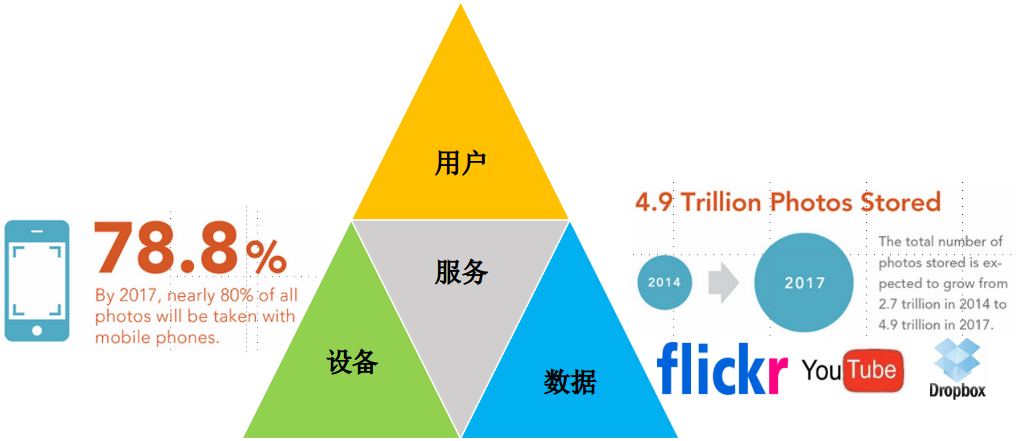
\includegraphics[width=0.9\textwidth]{social-media.png}
\caption{社交多媒体数据的产生和利用现状} \label{fig:status}
\end{figure}
然而,由于缺乏智能的社交多媒体数据建模和表达服务,这些海量的数据所包含的信息并没有得到
充分的挖掘和利用。如图~\ref{fig:status}所示,一方面,社交多媒体数据呈现出并保持着爆炸式的增长趋势;
另一方面,这些记录了珍贵记忆的用户数据被大量的存在本地或者云端磁盘上,
却很少再次被用户浏览。社交多媒体数据中所蕴含的故事性和社交性,并没有带来更好的用户体验。
随着人们对于多媒体内容品质和个性化需求的提高,越来越多的研究人员和工业界研究机
构投入更多的精力到社交多媒体数据中。
此外,由于社交多媒体数据的数量庞大,质量不确定、内容冗余、多样,
并带有丰富的社交信息,对相关的处理算法提出了更复杂的要求。
因此,对于社交多媒体数据的研究已成为计算机视觉领域的研究热点,相关的成果既有利于
推动计算机视觉以及多媒体领域相关课题的创新,
对于用户体验的提升以及工业界的发展都也具有重要的应用价值和现实意义。

\section{社交多媒体数据关键问题}
\label{sec:key_problems}
社交多媒体数据的研究涉及内容的语义理解以及应用层的关联表达两个大的方面。
其中,语义理解面临的主要问题包括:
\begin{itemize}
    \item 解决标注难的问题。机器学习算法可以归纳为有监督学习,
        半监督学习,和无监督学习三个类别。
        有监督学习通常能够获得最好的分类效果。然而,它依赖大量准确的标注数据,
        在当前大数据的背景下有监督学习的应用成本十分高昂。
        据了解,目前最大的有标注图片数据集ImageNet~\cite{russakovsky2015imagenet}
        花费了大约$25,000$名用户一年左右的时间完成标注。
        尽管如此,ImageNet仅包含$22,000$个类别,与现实应用中的语料库相差甚远(如WordNet
        ~\footnote{\url{http://wordnet.princeton.edu/}})。
        与之相反,半监督学习和无监督的学习不需要大量的标注,但是分类的效果与有监督学习
        还有明显的差距。 基于以上问题,
        越来越多的研究人员将注意力放在了弱监督学习上(Weakly Supervised
        Learning)。
        弱监督学习是指从标注不完备、不精确的大规模噪音数据中,
        充分挖掘有价值的信息,滤除或抑制错误信息,
        从而达到学习模型的目的。
        因此,弱监督学习能够充分利用大规模有噪音的标注数据,
        解决有监督学习标注难和无监督学习性能差的问题。

    \item 解决处理慢的问题。社交多媒体数据的规模十分庞大,
        对于模型的复杂度以及硬件的计算水平都提出了很高的要求。
        此外,移动设备的计算能力、存储空间以及电池容量依然有限,
        提高社交多媒体数据的处理速度对于提升移动端的用户体验至关重要。
        为了提升社交多媒体数据的处理速度,一方面可以利用特征选取(Feature
        Selection)的方法减少特征提取的种类和数目。
        图片或视频的内容既包括传统的全局特征,局部特征,
        也包括近年来提出的深度神经网络不同层产生的特征。
        对于不同的任务,有些特征具有很强的表现力,有些特征则十分冗余。
        因此,选取对具体任务最紧凑、最具有表征能力的特征作为数据内容的表达,
        可以减少特征提取的种类和数目,从而提高处理速度。
        另一方面,可以对特征提取过程中用到的模型进行简化,
        减少每种特征提取的时间开销。例如,近年来深度学习网络在图片识别,
        物体检测等领域取得了非常好的效果,但是网络的深度和参数数目也在不断增加,
        如何在不影响模型准确度的情况下简化深度网络模型已经成为了当前的热点问题。
\end{itemize}

社交多媒体数据关联表达是指根据用户个性化的需求,从社交多媒体数据中选择有关联的数据,
并以一定的表达形式将这些关联的数据呈现给用户。它面临的主要问题包括:
\begin{itemize}
    \item 内容的组织和选取。当前,社交多媒体数据以碎片化的形式,
        根据不同用户按照拍摄或上传的时间顺序存储在云端服务器上,
        社交网站以及搜索引擎根据根据用户提供的标签对数据进行索引,
        查询和检索。然而,社交多媒体数据存在质量不确定,内容冗余多样以及故事性等
        特点,高效的内容组织方式需要理解数据之间的关联性和故事性,从时间,位置,
        用户,内容,关联性等多个维度对数据进行组织。此外,针对用户个性化的需求,
        给用户返回最具有代表性的数据,同时返回低质量,重复的数据。
        例如,xxx系统。。

    \item 可计算的编辑语法。内容的组织和选取只是将数据高效地组织在一起,
        并选取最能满足用户需求的数据。然而在实际应用中,
        需要在原始的社交多媒体数据的基础上以一种新的、富有艺术美感的
        形式重新呈现给用户。例如,Magisto
        \footnote{\url{http://www.magisto.com}}
        系统能够给用户的图片和视频
        加上丰富的视频特效,并将视频和音乐的节奏进行匹配,生成一段
        类似专业编辑人员编辑的具有丰富表现力的音乐视频。
        专业的编辑人员在视频编辑中根据素材的内容以及需要表达的效果
        选取与之相适应的素材和特效对视频进行编辑,对于计算机,如何将
        专业编辑人员在编辑中运用到的规则和语法转化成可计算的规则和算法是
        社交多媒体关联表达面临的一个主要问题。由于表现形式以及编辑语法
        的多样性,挖掘和应用可计算的编辑语法也具有非常大的挑战性。

\end{itemize}

\section{本文的主要工作}
针对章节~\ref{sec:key_problems}中提到的关键问题,本文分别对社交多媒体数据
的语义理解和关联表达做了深入的研究,构成了社交多媒体数据挖掘和利用的一个相对
完整的框架。图~\ref{fig:correlation}给出了本文研究的具体内容以及相顾志坚的关联。
针对语义理解标准难的问题,弱监督深度学习可以直接从带有不准确标注的社交多媒体数据
中学习语义分类模型,理解数据的内容。结合传统计算机视觉方法和弱监督深度学习得到的
特征,特征选取针对具体的任务选取最紧凑,最有代表性的特征自己对数据内容进行表达,从而
减少特征提取的种类和数目,加快大规模社交多媒体数据处理的速度。此外,弱监督深度学习
需要耗费大量的计算资源,本论文结合特征提取算法,提出了深度模型简化算法,减少深度神经
网络的计算时间和参数个数。对于社交多媒体数据的关联表达,本文从照片集关联表达和多摄像头
视频自动剪辑两个方面做了具体的应用研究。其中,照片集关联表达对照片集中的事件进行分析
检测,根据照片的质量和关联选取有代表性的照片,通过可计算的视频编辑语法,对照片集
记性故事化的表达。移动多摄像头自动剪辑则将同一时间段同意地点不同用户拍摄的
多摄像头视频在时间上进行同步,通过可计算的视频编辑于法,选取镜头和录音,将多摄像头视频
剪辑成单一高质量的音视频流。

\begin{figure}[ht]
\centering
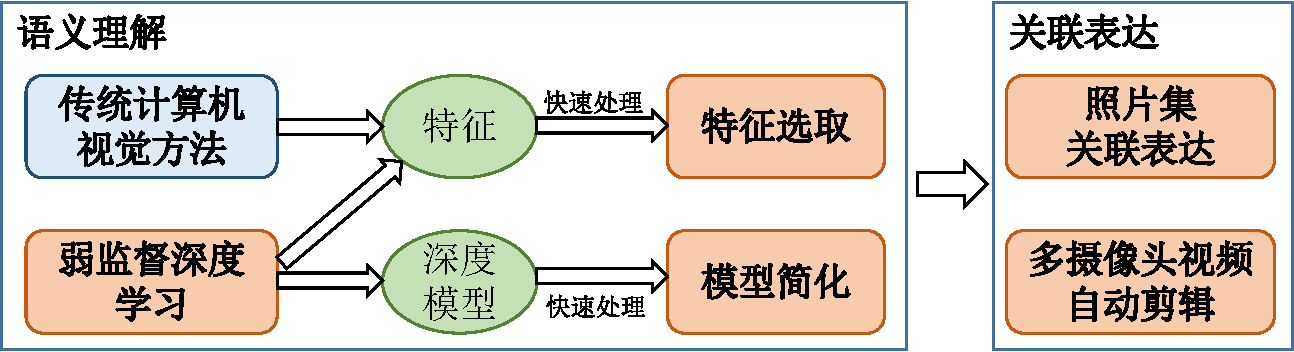
\includegraphics[width=0.9\textwidth]{correlation.pdf}
\caption{社交多媒体数据的研究内容和相互关联}
\label{fig:correlation}
\note{橙色部分表示本文的研究工作}
\end{figure}

基于以上研究点,本论文具体的研究内容包括:
\begin{enumerate}[{(1)}]
    \item 社交多媒体数据弱监督深度学习的算法研究: 针对任意的图像类别,
        从互联网抓取弱标注数据,提出具有抗噪效果的图片分类模型。
        传统深度学习算法对于噪声的敏感性是由于所有的数据在学习过程中具有相同的权重。
        本论文提出的方法的基本假设是:同一类别下,正确标注的图片由于语义上关联,
        在特征空间上比较接近,而错误标注的图片则与其他图片有很大的差异性。
        因此,我们可以利用图片在特征空间上的关系,
        使得不同的训练数据在训练过程中有不同的贡献加权,
        从而使得在特征空间上“孤立”的图片具有较小的权重,
        特征空间上密集区域的图片具有较大的权重,我们称之为相关反馈。
        该思想可以通过在学习中进行特征空间的低秩分解实现。
        为了加速模型训练的速度,我们进一步通过一系列的推导和近似,
        最终降低模型的复杂度,用于大规模社交多媒体数据的模型训练。

    \item 大规模高维特征选取算法研究:
        多媒体数据特征表述不仅包括高层次的卷积神经网络特征,
        还包含低层次全局特征(如颜色特征,纹理特征),局部特征(如SIFT,SURF)
        以及用来通过局部特征描述整体视觉信息的词袋特征等。
        实际应用中需要根据需求选取对目标任务最有用的特征子集,
        这对于大规模社交多媒体数据的处理速度以及移动设备有限的计算能力和内存空间尤其重要。
        此外,去除特定任务不相干的特征,还可以提高特征的表达能力。
        本论文提出从大规模高维数据中选取特征的高效算法。
        已有稀疏在线特征选取算法的复杂度与特征的维度成正比,
        本论文利用二阶在线学习算法,基于特征的置信度进行特征选择,
        并利用最大最小堆结构提出快速特征选取算法。
        由于置信度的单调递减特性,本文进一步提出了快速二阶在线特征选择算法,
        将算法的复杂度降为与非零特征数目成正比。

    \item 深度学习模型简化算法研究:
        深度卷积神经网络的深度和模型参数通常比较大,
        例如经典的VGG-16网络包含超过200M的模型参数。
        大量的模型参数意味着在实际应用中需要大量的计算资源和时间,
        极大地限制了深度神经网络在大规模图片检索和图片识别等任务上的应用。
        此外,深度网络在移动设备上的应用已经成为一种趋势。由于移动设备计算能力的限制,
        在不影响模型准确度的条件下简化深度网络模型已经成为迫切的需要。
        本论文提出一种基于在线特征选取的模型简化算法。算法主要针对卷积层进行简化,
        对每一个卷积层增加一个卷积核的权重层。
        初始条件下所有卷积核的权重为1,在学习过程中对权重进行更新,
        每次更新后利用稀疏在线特征选取算法将部分权重设为0,保留剩余的权重。
        区别传统方法,稀疏在线学习的方法可以在训练过程中动态的调整需要保留的卷积核,
        从而减小模型简化对模型参数的影响。

    \item 照片集关联表达算法研究:
        照片集的关联表达首先对照片集进行事件检测,找出用户所拍摄的不同事件。
        其次,利用弱监督的深度学习算法进行照片的内容分析和模型简化。
        由于深度网络的每一层都是对照片不同层次的语义表达,
        本文将这些特征拼接到一起组成高维特征,
        并利用本文提出的在线特征选取算法选取最能鉴别照片语义的特征子集,
        构成照片内容的最终表达。为了达到更好的表达效果,
        不同风格的照片需要采用不同的编辑技巧。
        本文设计了17个设计风格,并利用弱监督深度神经网络从网络上抓取训练图片,
        得到设计风格的分类器,将照片集中的事件分配到不同的风格中。
        最后,通过可计算的视频编辑语法,对照片进行动画特效处理以及音乐的匹配,
        最终生成具有关联表达能力的视频呈现给用户。

    \item 移动多摄像头视频自动剪辑算法研究:
        多摄像头视频是指在同一时间段,
        同一地点由不同摄像头拍摄的时间上有重叠的一组视频。
        多摄像头视频是不同的人从不同的角度对相同事件的记录。
        本文提出一个全自动的移动多摄像头视频自动剪辑系统。
        我们首先邀请专业的视频编辑人员探讨可计算的视频编辑语法。
        根据这些语法,自动剪辑系统首先对音频流进行质量评估,
        在保证尽可能减少音频流切换次数的条件下选取高质量的音频流,
        形成最终的单一音频流。对于视频流,首先将多摄像头视频进行语义分割,
        得到视频子镜头,其次对这些子镜头的视觉质量,运动,
        以及相互之间的多样性进行评估,最终在保证镜头运动一致性的前提下,
        最大化质量和多样性,选取视频镜头。对于镜头切换时机的选取,
        则根据音频的节奏以及语义特性,对切换频率进行匹配。
        系统最后将单一的音频流和单一的视频流进行混流,得到最终剪辑好的视频呈现给用户。
\end{enumerate}

\section{本文的主要创新点}
本论文的主要创新点有以下几点:
\begin{itemize}
    \item 针对社交多媒体数据标准难的问题,
        提出一种可以从互联网数据中学习图像类别的深度神经网络学习算法,
        摆脱了对大量标注数据的依赖。该算法利用数据本身之间的关联,
        使得不同的数据在模型训练中有不同的贡献加权。
        同时,通过一系列的推导和简化,最终的模型复杂度低,对于训练大量数据有重要意义。

    \item 针对大规模社交多媒体数据处理慢的问题,
        提出了从大规模高维数据中选取特征的高效算法。
        相比于已有的批处理算法和在线学习算法,该算法大大降低了特征选择的时间复杂度,
        同时,选取的特征具有和传统算法选出的特征差别不大甚至更好的表述能力。

    \item 针对深度模型处理慢,耗费计算资源的问题,
        提出了简化深度卷积神经网络的高效算法,将传统的多维数据组稀疏问题转化为
        经典的一维特征选取问题,在不影响模型准确率的情况下极大减少了模型参数。

    \item 提出了全新的照片集关联表达算法——Monet,
        从个人照片集中自动检测事件,选取有代表意义的图片,
        选取合适的视频编辑风格,并将设计师设计的视频编辑语法应用到照片集的编辑中。

    \item 提出移动多摄像头视频自动剪辑系统——MoVieUp,
        自动编辑移动多摄像头视频并生成一段综合音频视频流的方法。
        该方法首次考虑了音频流的剪辑,
        并且首次系统的讨论视频编辑理论在自动化方法中的应用。
\end{itemize}

\section{本文的结构安排}
本论文主要研究社交多媒体数据的语义理解和关联表达中的几个关键问题:弱监督深度学习,
特征提取,模型简化,以及照片集关联表达和移动多摄像头自动剪辑。各章节内容安排如下:
\begin{itemize}
    \item 第2章从弱监督学习,特征提取,模型简化,
        和关联表达四个方面介绍本论文相关工作的研究现状和工作基础。
        在弱监督学习方面,主要介绍了传统的弱监督学习方法和
        近年来热点研究的弱监督深度学习方法;在特征提取方面,主要回顾了传统的
        批处理方法,用于解决大规模流数据的在线学习方法,和在线特征提取算法;
        在模型简化方面,主要介绍与深度卷积神经网络相关的模型简化工作;
        在关联表达方面,主要介绍学术界和工业界关于社交多媒体数据的研究和代表性应用产品。
    \item 第3章重点介绍弱监督深度相关反馈网络的具体设计思路和实现方法,
        简化模型训练的理论证明和近似策略,以及相应的实验结果。

    \item 第4章介绍大规模社交多美数据快速处理的方法。
        首先介绍在线稀疏学习方法的基本模型,并介绍本文提出的
        置信度加权在线稀疏学习和置信度加权在线特征选取方法。
        本文从大规模标准数据集上验证算法的有效性,
        并在图片检索的实际任务中验证算法的可行性。
        其次,该部分介绍了深度学习模型简化的问题建模和具体算法,
        以及相应的实验结果。

    \item 第5章介绍照片集关联表达系统,包括照片集中事件检测方法,代表性图片选取
        算法及相应的质量评估,多样性评价,和时间均衡性考量。在选取的代表性图片上,
        系统基于弱监督学习算法设计了不同风格的分类器,将照片集中的事件分配到不同的
        风格中,利用针对不同风格设计的可计算的编辑语法,对照片赋予丰富的特效,生成
        具有表现力的视频,重现照片集中的场景和故事。

    \item 第6章介绍移动多摄像头自动剪辑系统。系统首先介绍针对移动多摄像头视频
        自动剪辑的可计算的视频编辑语法,并提出相应的系统框架。该部分详细介绍了
        音频的质量评估和剪辑方法,基于音频节奏和语义内容的视频切换点检测算法
        和基于镜头质量,多样性,和运动连续性的镜头选取算法。最后,通过实验证明
        了系统各个部分的有效性和整体的用户体验。

    \item 第7章对全文进行总结,以及未来可以进一步开展或改进的工作。
\end{itemize}

\chapter{国内外研究现状和工作基础}
随着智能手机及其他移动设备的普及,
社交多媒体数据的规模也呈现出了爆发式的增长。
对于社交多媒体数据的挖掘和利用已经成为了当前研究的热点问题,
相关的成果既有利于推动计算机视觉以及多媒体领域相关课题的创新,
对于用户体验的提升以及工业界的发展都也具有重要的应用价值和现实意义。

本文主要研究社交多媒体数据的包括包括语义理解和关联表达两个方面,涉及
弱监督深度学习,特征提取,模型简化,照片集的关联表达和移动多摄像头视频自动剪辑
几个关键问题。本章内容对这些关键问题的研究现状和工作基础做详细回顾。
首先回顾弱监督学习,总结近年来弱监督分类和弱监督深度神经网络的发展情况;
然后针对社交多媒体数据的特征提取, 回顾传统的批处理方法,
解决大规模流数据的在线学习方法,和在线特征提取算法,以及他们在
解决大规模社交多媒体数据特征提取问题中的问题和不足;
在模型简化方面,主要介绍与深度卷积神经网络相关的模型简化工作;
在关联表达方面,从照片集和移动多摄像头视频两个角度分别介绍学术界和工业界
的研究成果和代表性应用产品,指出他们在社交多媒体数据关联表达中
的不足,引出本文提出的照片集关联表达系统和移动多摄像头自动剪辑系统。

\section{弱监督学习}
弱监督学习是指数据标注不完备或者包含噪音条件下的分类问题。本文主要针对
弱监督图像分类问题做工作总结和算法创新。具体的方法可以分为两个方面:
数据去噪(Data Cleaning)和鲁棒噪音分类模型(Noise Robust Models)。

\subsection{数据去噪}
\label{sec:data-cleaning}
数据去噪是指找出并移除可能错误标注的数据。
数据去噪的优点在于它不依赖于目标任务的模型和训练方法。
但是数据去噪也面临区别噪音数据和异常数据的难题~\cite{danyluk2014small}。
数据去噪方法会导致两种类型的错误:正确标注的样本被误判为错误标注并被丢弃;
错误标注的样本被漏判。

经典的数据去噪方法只基于图片本身的视觉特征。
Brodley等人提出的交叉过滤法~\cite{brodley1999identifying}采用类似于交叉验证的思路,
将训练数据分成$n$等份, 并选择$m$种分类算法(称为过滤算法)。
对于每份数据,在剩下的$n-1$份数据上训练$m$个分类模型。
然后用得到的$m$个分类器对这部分数据进行预测,
最后通过一定的过滤算法判定错误标注的数据并将之移除。
最大边界难分类样本学习通过迭代地学习正负类别分界面,
保留难分类样本,移除易分类数据,从而更新正负样本集的方法
来达到去除噪音数据的目的~\cite{zhou2015conceptlearner}。

交叉过滤法和最大边界难分类样本学习算法直接利用弱监督的数据标注,属于
有监督学习方法。研究人员也提出了一些半监督的噪音数据去除方法。半监督学习方法
首先需要人工标注部分数据作为种子数据,记为$\L = \{(\x_i, y_i)\}_{i=1}^m$。剩下
的数据记为$\U = \{\z_j\}_{j=1}^n$。通常情况下,$m \ll n$。
核平均算法的核心思想是通过对未标注的数据进行加权,
使得加权后的数据分布与有标注数据的分布相同~\cite{huang2006correcting,vo2015deep}。
直推式支持向量机(Transductive Support Vector Machine, TSVM)
~\cite{sindhwani2006large,vo2015deep}
同时根据有标注的数据$\L$和未标注的数据$\U$寻找分界面,
并约束最多有$r$个未标注数据被判定为正类样本。

此外,由于社交多媒体数据具有丰富的上下文(context)信息,
这些上下文信息也从侧面反映了图片的语义内容, 因此可以用来辅助数据去噪。
Schroff等人提出了一种基于图片在网页中的文本上下文信息以及
图片本身的视觉特征对图片进行重排序的算法~\cite{schroff2011harvesting}。
算法首先利用图片附近的文本上下文学习标注是否正确的后验概率并进行重排序。
然后从基于文本的重排序中选择前$n_+$个图片作为正样本,
再从所有其他类别的图片中选择$n_-$个图片作为负样本。对图片提取视觉特征以后,
训练一个SVM分类器。社交主动学习(Social Active Learning)首先用视觉特征训练
分类器,并评价数据对于提升分类效果的信息量,同时利用文本特征评价每个数据标注可靠
的置信度,综合考虑信息量和置信度选取数据,
迭代地训练模型并选取正确标注的数据~\cite{chatzilarisalic}。

可以看出,数据去噪方法分成两步进行:特征提取和数据去噪的模型训练,
对于噪声的判别也依赖于人为假设和定义的准则,这些因素导致在真实的
社交多媒体数据上,数据去噪方法的效果受多重因素影响,很难达到理想的效果。因此,
我们需要提出一些端到端的学习方法(End-to-End Learning),并利用数据之间的关联
达到弱监督学习的目的。

\subsection{鲁棒噪音模型}
鲁棒噪音模型是指本身对噪音数据不敏感或具有抑制作用的模型。
在经验风险最小化(ERM)规则和给定的损失函数下,
如果模型发生分类错误的概率保持不变并且与标注噪音无关,
则认为模型是对标注噪音鲁棒的。研究人员讨论了在特定条件下,理论上是否存在
对标注噪音完全鲁棒的模型~\cite{manwani2013noise}。 例如,
$0-1$损失函数在均匀的标注噪音或者能达到$0$错误率的情况下是
噪音鲁棒的~\cite{thathachar2011networks,sastry2010team}。
Beigman等人讨论了非随机噪音模型下的鲁棒模型~\cite{beigman2009learning},
最小平方差损失函数在均匀标注噪音下同样是噪音鲁棒的。其他常见的损失函数,如
指数损失函数,对数损失函数,以及Hinge Loss均不是噪音鲁棒的。换句话说,大部分常见的
机器学习算法都不是完全噪音鲁棒的,但可以在一定程度上减小错误标注的影响, 提升
模型的鲁棒性。

对于经典的SVM分类器,Bunescu等人提出了稀疏多实例学习算法用于解决训练样本中的
噪音数据问题~\cite{bunescu2007multiple,vijayanarasimhan2008keywords}。
多实例学习将一组包含正样本包的有噪音数据称为一个正样本包,将一组负样本数据称为负样本包,同时假设正样本包
中至少包含一个真实的正样本,负样本包中全是负样本。通过对正负样本包采用
不同的约束条件和惩罚稀疏,达到抑制噪音影响的目的。

逻辑回归是一种经典的概率统计分类模型。 相比于其他分类模型(如SVM),
逻辑回归的能够输出样本是否为某个类别的概率,因此得到了十分广泛的应用。
然而,逻辑回归算法对于训练数据中的噪音标注十分敏感。
Feng等人提出了一种基于次高斯分布的鲁棒逻辑回归算法~\cite{feng2014robust}。
根据理论分析结果,算法首先去除范数大于一定阈值的数据,
在剩余的数据中仅最大化前$n_1$数据的标注和预测结果之间的相关度。
在随机噪音(Noise at Random, NAR)假设下,研究人员提出用隐藏变量对数据的真实类别,错误标注的转移概率
以及他们与观测到的标注之间的关系进行建模,
并通过EM算法优化目标结果~\cite{izadinia2014image,izadinia2015deep}。

近年来,深度卷积神经网络在图片识别上获得了巨大的成功。
卷积神经网络最早于1998年被Lecun等人运用在了文字识别上~\cite{lecun1998gradient}。
随着显卡能力的提升,,
得益于显卡设备的快速发展,卷积神经网络的深度、宽度以及结构不断改进,
深度卷积神经网络的识别能力和应用范围都得到了巨大的
提升~\cite{krizhevsky2012imagenet,simonyan2014very,szegedy2015going,szegedy2016rethinking,szegedy2016inception,he2016deep}。

然而,深度卷积神经网络需要大量的训练数据,对于数据标注的质量有很大的依赖性。
如何利用容易获得的大量弱监督数据训练深度卷积神经网络成为了近年来的研究热点之一。
自举深度神经网路是2014年谷歌研究团队提出的利用图片特征之间的相似性
监督网路学习,抑制错误标注影响的学习方法~\cite{reed2014training}。文章
认为,如果图片的特征之间具有相似性,那么预测的结果同样也应该比较类似,
并称之为感知连续性。在随机噪声的假设下,在神经网络中加入全连接隐藏层表示真实的
类别,为了达到感知连续性的约束,论文提出引入类自适应编码器的方法训练网络。此外,还可以
通过约束隐藏层输出的熵最小达到软自举优化的目的,
以及约束隐藏层概率最大类别的熵最小达到硬自举的目的。Sukhbaatar等人则通过约束
隐藏层参数的迹来达到感知连续性的优化目标~\cite{sukhbaatar2014training}。
Xiao等人则综合考虑了标注可能遇到的随机噪音和非随机噪音,通过隐藏变量对不同噪音
类型下的概率进行建模,用两个神经网络分别学习噪音类型和真实的标注,通过EM算法
学习整个模型的参数~\cite{xiao2015learning}。
以上方法都基于特定的噪音模型, Azadi等人提出
一种辅助图片正则项(Auxiliary Image Regularizer, AIR)的方法~\cite{azadi2015auxiliary},
根据数据的特征结构,通过组约束的方法使得只有部分数据具有响应,
从而在训练数据中识别出有用的辅助数据,更好地训练神经网络。某种程度上,
可以认为辅助图片正则项方法是在训练数据中寻找最近邻数据,
减少深度模型对噪音数据的拟合。

传统的鲁棒噪音模型方法仍然基于特征提取和模型训练两个步骤,
具有章节~\ref{sec:data-cleaning}提到的局限性。现有的弱监督深度学习
方法基于特定的噪音模型,难以处理真实的场景,或建模过于复杂,难以
训练。AIR方法利用图片之间的相似性抑制噪音,但组稀疏优化提高了
网络训练的难度和时间开销。因此,我们提出一种新的利用数据在特征空间的关联性
进行相关反馈的弱监督深度神经网络,并对网络进行简化和近似,提高模型的
适用性和实用性。

\section{特征选取}
图像特征表述不仅包括高层次的卷积神经网络特征,
还包含低层次全局特征(如颜色特征~\cite{jain1996image},
边缘特征~\cite{jain1996image} ,纹理特征~\cite{manjunath1996texture}),
局部特征(如SIFT~\cite{lowe1999object} ,SURF~\cite{bay2006surf})
以及用来通过局部特征描述整体视觉信息的词袋方法等~\cite{yang2007evaluating}。
实际应用中需要根据需求选取对目标任务最有用的特征子集,
这对于计算能力,内存,和电量都十分受限的移动设备尤其重要。
此外,去除特定任务不相干的特征,还可以提高特征的表达能力。
特征选取在机器学习和数据挖掘领域得到了广泛的研究,
可以分成两类:批处理方法和在线特征选取。

\subsection{批处理方法}
批处理方法是指每次迭代都需要考虑所有的训练数据,可以分为三个类别:
\begin{itemize}
    \item 过滤法: 过滤法分析特征之间的关联,距离,交互信息熵等,
        选取最有代表意义的特征子集~\cite{yu2003feature,jiang2015relative,li2016feature} 。
        Yang等通过分析指出,传统的过滤法存在单调性的问题,
        不同大小的特征子集之间存在单调的包含关系,
        这种包含关系在实际情况中并不成立~\cite{yang2013efficient}。
        他们对特征之间的联系进行建模,提出了一种多核学习的方法。
    \item 包装法: 包装法使用预先定义好的分类器去评价
        选取的特征子集的性能~\cite{kohavi1997wrappers}。
        这类方法迭代的选取不同的子集,并得到该子集在对应分类器上评价指标,
        虽然能够获得该分类器上最好的特征子集,但是计算的开销也十分巨大,
        因此对于该类方法的研究相对较少。
    \item 嵌入法: 嵌入法将特征选取与模型训练进行融合,
        是一种在高效的过滤法和高准确率的包装法之间
        综合平衡的方案~\cite{pappu2015sparse,le2014feature}。
\end{itemize}

\subsection{在线特征选取}
批处理方法的缺点在于需要将所有训练数据都加载到内存中,
对于目前的大量高维数据,这类方法的局限性十分明显。
同时,批处理方法要求数据预先已经全部存在,实际场景中,存在大量的流媒体数据。
因而近年来,随着数据量的增大和维度的增加,大量的工作转向了在线学习。
最早的在线学习算法是1958年提出的感知机算法。
2006年,Crammer等人在感知机算法上增加约束,
使得模型在每次迭代后在当前数据上都能获得正确的分类结果~\cite{crammer2006online}。
考虑到批处理学习算法中,二阶海森矩阵能够显著提高算法的收敛速度,
Crammer等人假设模型参数服从一个高斯分布,用协方差矩阵表示当前模型对于参数的不确定性,
提出了置信度加权的在线学习算法CW~\cite{crammer2009multi}。
该算法每次迭代时约束更新后的模型以一定概率在当前的数据上获得正确的预测结果。
由于该算法假设数据的标注都是正确的,在实际场景中的效果会收到影响。
自适应的置信度加权在线学习算法则降低了对于噪音数据的敏感性~\cite{crammer2009adaptive}。

近几年,在线学习被应用到特征选取上。Langford等人提出的稀疏在线学习算法,
在感知机模型上增加了模型参数的L1范数作为正则项,
获得稀疏的模型~\cite{langford2009sparse}。
Duchi等提出的FOBOS算法将稀疏在线学习分成两步,第一步是正常的在线学习,
第二步优化目标使得模型尽可能接近第一步得到的参数,
同时对应的L1范数最小~\cite{duchi2009efficient}。
另一种思路则是优化模型在主空间和对偶空间的距离,
利用模型的L1范数达到稀疏模型的目的而提出的RDA算法~\cite{xiao2010dual} 。
RDA算法在高稀疏条件下往往能获得更好的特征表达能力。
受置信度加权等二阶算法的启发,Duchi等利用梯度的协方差构建二阶信息,
提出了自适应的二阶FOBOS算法和RDA算法。

基于L1范数的稀疏在线学习算法是针对特征选取的一种“软”约束。
参数设定与目标特征数目之间没有确定的关联。
基于L0范数的在线特征选取也得到了研究人员的关注。
Wu等提出的在线特征流学习能够在每次迭代后返回一个模型和它选取的特征子集~\cite{wu2010online}。
该算法假设每次获得所有数据的某个特征,不同特征按照时序被送到算法中。
另一种更普遍的应用场景下,算法每次可以获取一个数据的部分或者所有特征,
不同数据按照时序到达算法。Huang等提出一种无监督的在线特征选取算法处理这类数据~\cite{huang2015unsupervised}。
Wang等则利用有监督的数据,根据权重向量的绝对值进行在线特征选取~\cite{wang2014online}。

批处理方法的主要问题在于不具有可伸缩性(Scalability),以及对于流数据不具有
很好的应对能力。基于L1范式的在线稀疏学习方法对于特征的数目不能做直接的约束,
在实际应用中需要根据不同的数据调整参数达到选取预期特征数目的目的。当前的在线
特征选取算法根据权重向量绝对值选取特征的做法与批处理方法的效果还有较大差距,并且
算法的复杂度较高。因此,本论文提出了大规模高维特征选取算法,不仅具有与批处理方法
相近的准确率,也极大地减小了计算复杂度,对于处理大规模社交多媒体数据具有非常大
的应用价值。

\section{模型简化}
近年来,深度卷积神经网络在图片识别,物体检测等领域获得了巨大的成功,
为了进一步提高网络的表征能力,研究人员不断改进网络的
深度~\cite{simonyan2014very},
宽度~\cite{zagoruyko2016wide}以及
拓扑结构~\cite{szegedy2015going,srivastava2015highway,he2016deep}。
然而,大量的网络参数也要求大量的时间开销和计算资源,也极大地限制了
深度网络在计算能力、存储空间和电池续航受限的移动设备上的应用。如何在
不影响网络性能的情况下减少网络参数成为了当前的研究热点问题。深度网络模型简化
相关的工作可以分为三个类别:矩阵分解、量化以及稀疏优化。

矩阵分解利利用参数之间的相关性,对参数矩阵进行低秩分解,从而减少网络的参数个数。
Denil等人提出将参数矩阵分解成两个低秩矩阵的乘积,将其中一个矩阵作为特征空间的一组基,
并提出了基向量字典的构建方法~\cite{denil2013predicting}。
Denton等人提出在网络的预测阶段,用奇异值分解(Singular Vector Decomposition, SVD)
对参数矩阵进行分解,如果参数矩阵的奇异值迅速下降,则参数矩阵能够被
前最大$t$个奇异值及对应的奇异向量很好地近似~\cite{denton2014exploiting}。
Rigamonti等人提出的方法在空间上对每个通道的卷积核用秩为$1$的矩阵进行近似, 从而减小
计算量~\cite{rigamonti2013learning},Jaderberg等人在空间分解的基础上进一步利用
通道之间的冗余信息,将原始的卷积操作分解成两步卷积运算~\cite{jaderberg2014speeding}。
Ioannou等人和Tai等人进一步改进并扩展低秩分解方法,
将其用于更大的深度网络~\cite{ioannou2015training,tai2015convolutional}。
Mamalet等人将卷积核分解为秩为1的向量乘积,并与后续的池化(Pooling)操作冗合为
一层卷积运算,从而减少运算量~\cite{mamalet2012simplifying}。

量化是指利用较少的比特数表示网路参数,从而减少模型的大小以及乘法运算的复杂度。
目前常用的网络参数都采用32比特的浮点型数据,研究表明,
可以利用更少的比特数来表示每个参数。例如,Hwang等人和Arora等人提出仅用$+1, -1,
0$三个数值表示网络参数训练卷积神经网络~\cite{hwang2014fixed,arora2014provable}。
Courbariaux等人和Rastegari等人则进一步提出用二个数值
表示网路参数~\cite{courbariaux2015binaryconnect,rastegari2016xnor}。
Gong等人提出用向量量化的方法对全连接层的参数进行量化~\cite{gong2014compressing}。
针对卷积层的向量量化则在Wu等人提出的Q-CNN得到研究和应用~\cite{wu2016quantized}。
Anwar等人用最小平方差的方法量化网络~\cite{anwar2015fixed}。
Chen等人利用哈希函数随机将网络参数分组,达到量化的目的~\cite{chen2015compressing}。

当前网络的参数矩阵是密集矩阵, 稀疏优化的目标是使得最终的参数矩阵稀疏,
从而达到模型简化的目的。
区别于参数矩阵低秩分解,Liu等人提出对卷积核进行稀疏分解,并提出了高效的系数矩阵
相乘算法~\cite{liu2015sparse}。受L1或L2约束的启发,Han等人提出重复交替进行
删除神经元之间连接和重新训练精简后网络~\cite{han2015learning,han2015deep}。
然而,这些稀疏方法产生的稀疏性不是结构化的,运算时会导致无规则的内存访问,
不能带来实际的运算加速。Li等人根据卷积核的绝对值之和去除部分卷积核,从而
达到运算的加速~\cite{li2016pruning}。
Murray和Chiang运用结构化稀疏方法约束隐藏层神经元的个数~\cite{murray2015auto}。
Anwar等提出了卷积核,通道,以及卷积核内部的结构化稀疏方法~\cite{anwar2015structured}。
他们还提出用粒子滤波器(Particle Filter)衡量网络连接的重要性,从而
优化网络结构。Wen等人系统讨论了结构化的稀疏算法,从卷积核,通道,卷积核形状,
深度四个方面对网络进行进行结构化的约束,
不仅达到了减少网络参数的目的,还获得了实际运算速度上的提升。
Hu等人通过研究发现大网络的部分神经元的响应大部分情况下为0,且与网络的
输入信号无关。因此,他们通过分析网络神经元在大数据集上的响应去除部分
神经元~\cite{hu2016network}。
这些结构化的方法稀疏后的网络,有连接的神经元之间在通道上仍然是密集连接,
Soravit等人提出了对通道稀疏连接的方法,在保持其他结构化方法同样计算
速度的情况下获得了很好的效果~\cite{changpinyo2017power}。

以上介绍的模型简化方法,虽然取得了一定的效果,但同时也存在很多的问题。
矩阵分解方法对于全连接层以及大卷积操作具有非常好的效果,然而最新的网络
更倾向于使用更少的全连接层,并通过级联小卷积核的方法达到大卷积核同样的
感知野,不仅减少了运算量,还提高了网络的表征能力~\cite{szegedy2016rethinking}。
量化方法需要特定的硬件或软件库的支持才能显著提高运算的速度。
非结构化的稀疏优化方法对于减少参数数目作用比较明显,对于计算速度的提升十分有限。
结构化的方法一般基于参数的绝对值决定参数的重要性,具有一阶在线学习方法同样的
缺陷,而组稀疏优化的方法则增加了网络优化的难度。为此,有必要提出一种
新的模型简化方法,既能保证简化后网络的表征能力,实际提升网络的运算效率,
减少参数规模,又易于优化,提高模型简化的可操作性。

\section{社交多媒体数据的关联表达}
本节从照片集关联表达和视频关联表达两个方面回顾社交多媒体数据关联表达相关的工作。

\subsection{照片集关联表达}

照片集的关联表达涉及事件检测(Event Detection),关键照片选取,
和照片故事表达。通常,用户照片包含拍摄时的时间戳和位置信息,
我们可以利用这些信息将照片集分成不同的事件。Platt等人提出用
一个小时或者自适应的时间间隔作为相邻事件之间的时间间隔~\cite{platt2003phototoc}。
Graham等人扩展了该方法,使用事件聚类的类内内拍照频率和
类间时间间隔调整已有的事件划分~\cite{graham2002time}。
Gargi提出将拍摄频率的急速增加的时间点作为时间的起点,将长时间间隔没有拍摄
作为事件的终点~\cite{gargi2003modeling}。Matthew等人将可信度,动态规划
或者贝叶斯信息准则(Bayes Information Criterion, BIC)运用到照片的
相似度矩阵,从而检测事件的边缘位置~\cite{cooper2005temporal}。
一般来说,事件检测问题可以表示为一个聚类问题。Loui和Svakis提出用
2类的K-means聚类算法将照片分组,并检查照片之间颜色的相似性改进
聚类~\cite{loui2000automatic}。Gong等人利用层次聚合聚类算法将照片
分配到不同的聚类中心~\cite{gong2007segmenting}。
Platt等人用隐马尔科夫模型聚类~\cite{platt2003phototoc}。
Mei等人在时间,位置以及内容特征上利用混合高斯模型解决事件检测问题~\cite{mei2006probabilistic}。
Xu等人进一步利用纹理和深度特征改进了这个算法~\cite{shen2016multi}。

近年来许多研究工作和产品相继出现,用以解决关键照片选取问题。在学术界,
关键照片选取主要依赖照片的代表性~\cite{cooper2005temporal,mei2006probabilistic,shen2016multi,chu2008automatic}。
Cooper等人将事件中第一张照片作为关键照片。Mei
等人选择具有最大后验概率的照片~\cite{mei2006probabilistic}。
Chu等人提出在照片的聚类中,根据近似图片对之间的相互关系决定关键照片~\cite{chu2008automatic}。
Xu等人则根据事件的重要性引入了照片的受欢迎程度(popularity)以及时间内部的相似度决定
关键图片~\cite{shen2016multi}。

照片故事表达一直以来受到了工业界和学术界共同的关注。
例如,Magisto\footnote{\url{http://magisto.com}}和
Animoto\footnote{\url{http://animoto.com}}是两个可以根据用户提供的照片产生
音乐视频(Music Video)的在线服务。然而,它们依赖用户主动选取和提供的照片,
不能直接从照片集中总结并整理出故事呈现给用户。此外,用户需要手动指定
音乐视频编辑的风格。其他的在线服务,如Microsoft
Onedrive\footnote{\url{https://onedrive.live.com}},
Google\footnote{\url{https://plus.google.com}}可以在一定程度上对照片集进行
事件检测和照片选取,并且缺乏对数据的重新表达。
在学术界,Hua等人提出的Photo2Video系统是从照片产生视频
的先驱性工作~\cite{hua2006photo2video},利用相继运动将静态照片转换成运动片段,
最终通过转场效果并与节奏匹配生成最终视频。
然而该系统没有设计不同的编辑风格,所采用的编辑效果也比较单一, 其他系统比如
Tiling SlideShow系统将照片和背景音乐同步,
并以瓷砖式幻灯片的方法播放~\cite{chu2007tiling}。
Kuo等人提出的Sewing Photos系统专注于解决在播放照片幻灯片时,
给照片之间分配平滑的转场效果~\cite{kuo2011sewing}。
Sewing Photos和
Tiling SlideShow也存在Photo2Video同样的编辑效果单一的问题。
Yang等人提出了一种从照片中自动生成有吸引力的版面设计的算法。

以上系统没有系统对照片集进行总结整理,在表达时
很少运用丰富的视频制作特效和视频编辑风格和编辑语法,因而对于照片故事
的表现能力十分有限。因此,我们需要提出一个能够对照片集进行事件挖掘和关键图片选取,
并运用专业的编辑语法对故事进行再现表达,提供更为有效的照片集关联表达方法。
在表格~\ref{tab:monet-comp}中,我们比较了现有照片集关联表达系统和本文提出的Monet系统之间的差异。

\begin{table}[htbp]
    \centering
    \caption{照片集关联表达系统比较} \label{tab:monet-comp}
    \begin{tabular}{|c|c|c|c|c|}
    \hline
     & Magisto  & Animoto &  Google+ & Monet (this paper)\\
    \hline
    相机运动分析 & + & - & - & +  \\
    视频分析    & - & - & - & + \\
    人脸检测识别 & + & - & + & + \\
    场景分析 & + & - & + & + \\
    物体识别 & - & - & + & + \\
    音乐分析 & + & - & - & + \\
    照片分组和选取 & - & - & + & + \\
    设计风格 & + & - & - & + \\
    色彩调整 & + & + & + & + \\
    社交和云存储 & - & - & + & +  \\
    \hline
\end{tabular}
\end{table}
\subsection{移动多摄像头视频关联表达}
移动多摄像头视频是指在同一个事件中,有多个移动摄像头从多个角度拍摄的,时间上有
重叠的一组视频~\cite{DBLP:conf/mm/ShresthaWWBA10}。
随着智能设备的普及与性能的提升,移动多摄像头视频的自动剪辑成为了近年来
的热点问题。

移动多摄像头视频的自动剪辑的方法可以总结为三个类别:
基于规则的~\cite{DBLP:books/daglib/0023820},
基于优化的~\cite{DBLP:conf/mm/ShresthaWWBA10},
和基于学习的~\cite{DBLP:conf/mm/NguyenSNO13,DBLP:conf/mm/SainiGYO12}。
基于规则的方法模仿专业视频人员的编辑过程。然而,移动多摄像头视频的自动剪辑
过程更类似于用户的选择倾向,而并非固定的编辑规则。Shrestha等人提出了从
视频质量,多样性和切换点的合适度进行镜头选取的优化算法~\cite{DBLP:conf/mm/ShresthaWWBA10}。
然而实际系统中,论文并没有提出切实可行的切换点合适度的评价方法,仅仅
考虑了视频质量和多样性。在视频质量评估中,没有考虑到移动视频中的倾斜和遮挡问题。
此外,作者通过贪心算法解优化方程,仅获得了目标方程的局部最优解。
Saini等人提出Jiku Director用于解决在线视频剪辑问题~\cite{DBLP:conf/mm/NguyenSNO13,DBLP:conf/mm/SainiGYO12}。
他们通过学习隐马尔科夫模型(HMM)用于镜头选取和确定镜头长度。
然而,通过这种方式学习到的规则与内容无关,而实际中,镜头角度和长度的
选取都是和内容密切相关的,并且受运动强度,音乐的节奏,
以及其他因素的影响~\cite{DBLP:conf/mm/HuaLZ04a}。此外,该系统由于不能准确判断
视频的角度,因而不能做到全自动的视频剪辑,尤其是在模型的训练阶段,需要人工的干预。
Arev等人最近提出了从多摄像头视频的自动编辑系统~\cite{Arev:2014:AEF:2601097.2601198},
但是该系统十分依赖场景的三维重建,不适用于移动多摄像头。

以上系统均没有考虑音频的剪辑,而完整的视频是有音频流和视频流两部分构成的,
高质量的音频流对于提升用户体验具有十分重要的作用。
在表格~\ref{tab:mashup-comp}中,我们比较了现有移动多摄像头视频系统和本文提出的MoVieUp系统之间的差异。

\begin{table}[htbp]
    \centering
    \caption{视频自动剪辑系统比较} \label{tab:mashup-comp}
    \begin{tabular}{|c|c|c|c|}
    \hline
     & MoVieUp (this paper) & VD~\cite{DBLP:conf/mm/ShresthaWWBA10}
     & Jiku~\cite{DBLP:conf/mm/SainiGYO12}\\
    \hline
    diversity & Yes & Yes & Yes \\
    shakiness & Yes & Yes & Yes \\
    tilt & Yes & No & Yes \\
    occlusion & Yes & No & Yes \\
    audio mashup & Yes & No & No \\
    cut point & Audio+Video & Manual & Learning \\
    \hline
\end{tabular}
\note{VD is short for Virtual
    Director~\cite{DBLP:conf/mm/ShresthaWWBA10}. Transition matrix for cut points learnt by Jiku Director is the same to
    all videos, thus not content-based.}
\end{table}

移动多摄像头自动剪辑还与视频编辑相关,包括视频摘要(Video Summarization),
相机选取,以及家庭或音乐视频编辑。视频摘要与视频剪辑的共同点在于它们都要最大化
有信息内容的部分。Sundaram等人提出了从可计算的镜头中生成快速概览的
实用框架~\cite{sundaram2002computable}。该论文将视觉编辑语法运用到镜头编辑中(选取,
缩放,时长,顺序等)~\cite{CinemaElements1982},对于本文的工作具有很大的借鉴意义。

可计算镜头的检测通常基于人类记忆的一个仿真模型~\cite{sundaram2002computable}。
相机选取在演讲和会议等诸多特定场景都得到了广泛的研究,
通常可以通过识别演讲者或者检测人脸来选取需要展示的相机内容~\cite{DBLP:journals/ieeemm/LampiKBE08,sumec2006multi}。
Ranjan等人和Zhang等人提出的系统中用跟踪和基于音频的定位来选择相机。以上系统都可以
归结为基于音频的方法。在移动多摄像头视频自动剪辑中,音频不是唯一的关注点,音频定位和人脸检测
在嘈杂的拍摄环境以及低视觉质量的条件下的应用能力十分有限。

此外,还有大量关于家庭视频或音乐视频编辑的工作。Hua等人提出了自动家庭视频编辑系统
AVE,从一系列的家庭视频中提取一部分最精彩的镜头~\cite{DBLP:conf/mm/HuaLZ03}。
他们提出了两套规则分别保证对原来视频的代表性,以及音频和视频之间的协调性。
类似的方法被拓展到自动音乐视频编辑,该系统分析视频的时序结构和音频的节奏并进行匹配~\cite{DBLP:conf/mm/HuaLZ04a}。
然而,由于移动多摄像头视频需要进行时间上的同步,并且需要保证内容上的
质量和多样性,这些系统不能直接用于移动多摄像头视频自动编辑。


\chapter{弱监督社交多媒体数据语义理解}
    弱监督社交多媒体数据语义理解是指在训练数据标注不准确的条件下的语义理解。
    弱监督社交多媒体数据语义理解是分析挖掘利用社交多媒体数据的基础,本文后续部分的特征提取
    和关联表达都是基于弱监督社交多媒体数据予以理解的结果。
    本章主要研究弱监督目标识别问题。

\section{弱监督目标识别问题建模}
在目标识别问题中, 给定$n$个训练数据$X=\{(\x_1, y_1), \ldots,
(\x_n, y_n)\}$, $\x \in \R^d$是训练数据的特征表示,$y \in
\Y$是数据的类别, $|\Y| = K$是数据的类别空间,类别数目为$K$。
$y$的取值通常为离散的整数值。 本文仅讨论单类别分类问题,即每个训练数据有且仅有一个类别。

传统的目标识别问题假设数据的标注$y$是准确无误的,
在社交多媒体数据中实际获得的标注$y$
和真实的数据类别$z$存在不一致的情况。在统计学上,
用一个二值的随机变量$E$表示是否存在标注噪音。
数据$X$, 真实标注$Z$,
实际观测到的标注$Y$,和随机变量$E$之间存在图~\ref{fig:noise-taxonomy}
所示三种关系~\citep{frenay2014classification}。

\begin{figure}[ht]
    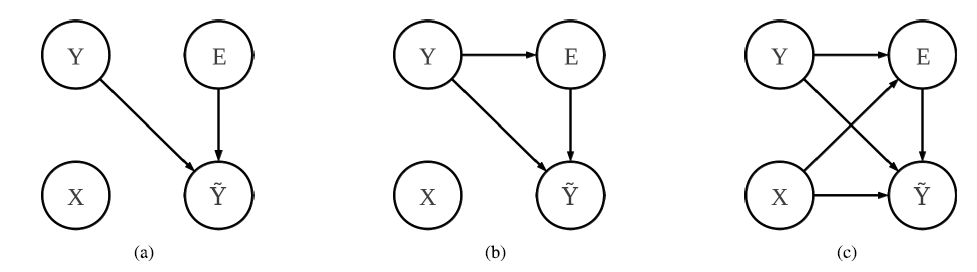
\includegraphics[clip=true, width=0.95\textwidth]{noise-taxonomy.png}
    \caption{数据标注噪音类型: (a)完全随机噪音; (b) 随机噪音; (c) 非随机噪音}\label{fig:noise-taxonomy}
\end{figure}

\begin{itemize}
    \item \textbf{完全随机噪音(NCAR)}:
        噪音$E$独立于其他随机变量,包括真实的标注$Z$。
    \item \textbf{随机噪音(NAR)}:
        噪音$E$独立于数据$X$, 但依赖真实的标注$Z$。该模型允许非对称噪音,
        即某些类别的数据更有可能出现标注噪音。随机噪音可等价地表示为一个标注矩阵或转移矩阵:
        \begin{eqnarray}
            \gamma =
            \begin{pmatrix}
                \gamma_{11} & \cdots & \gamma_{1K} \\ 
                \vdots & \ddots & \vdots \\ 
                \gamma_{K1} & \cdots & \gamma_{KK}
            \end{pmatrix}
            =
            \begin{pmatrix}
                \P(Y = 1|Z=1) & \cdots & \P(Y= K|Z=1) \\ 
                \vdots & \ddots & \vdots \\ 
                \P(Y = 1|Z=K) & \cdots & \P(Y = K|Z=K)
            \end{pmatrix}
        \end{eqnarray}
    \item \textbf{非随机噪音(NNAR)}: 上述两种噪音类型均假设标注噪音对于同一类别下的
        所有样本具有相同的影响。然而在实际场景中,上述假设不一定成立。例如,
        当样本与其他类别样本之间的距离较近时,更有可能发生错误标注。此外,
        样本分布密度较低的区域标注的可靠性也比其他区域低。在图~\ref{fig:noise-taxonomy}(c)所示的
        模型中,标注噪音$E$同时依赖于数据$X$和真实类别$Y$,错误标注更有可能
        出现在某些类别和数据空间的某些区域。非随机噪音是最有普适性
        的噪音类型。例如,分界面附近和低样本密度分布区域的标注噪音只能用非随机噪音
        来建模。
\end{itemize}

\section{相关反馈弱监督深度神经网络}
传统弱监督目标识别算法需要人工设计
一系列的特征,如全局特征(HOG),局部特征(SIFT, SURF)等。这些特征的表达能力直接
影响到图片分类的效果,不仅提高了研究人员设计特征的难度,也制约了目标识别效果的
提高。
近年来,深度卷积神经网络在图片识别上获得了巨大的成功。
2012年,Alex等人将深度卷积神经网络应用到了百万级规模的ImageNet图像识别任务上,
提出了AlexNet网络模型,通过5层的卷积神经网络,
直接从原始的图片像素中提取从浅层语义到深层语义的特征,
然后用3层的全连接神经网络作为分类器~\cite{krizhevsky2012imagenet}。
深度学习的优点在于不需要人工设计图片特征,网络通过反向传播的方式同时
学习特征提取和分类器。然而,经典的深度卷积神经网络对于数据标注的质量有很大的依赖性,
如何利用大规模弱监督社交多媒体数据训练深度卷积神经网络成为了近年来的研究热点之一。

\begin{figure}[ht]
    \center
    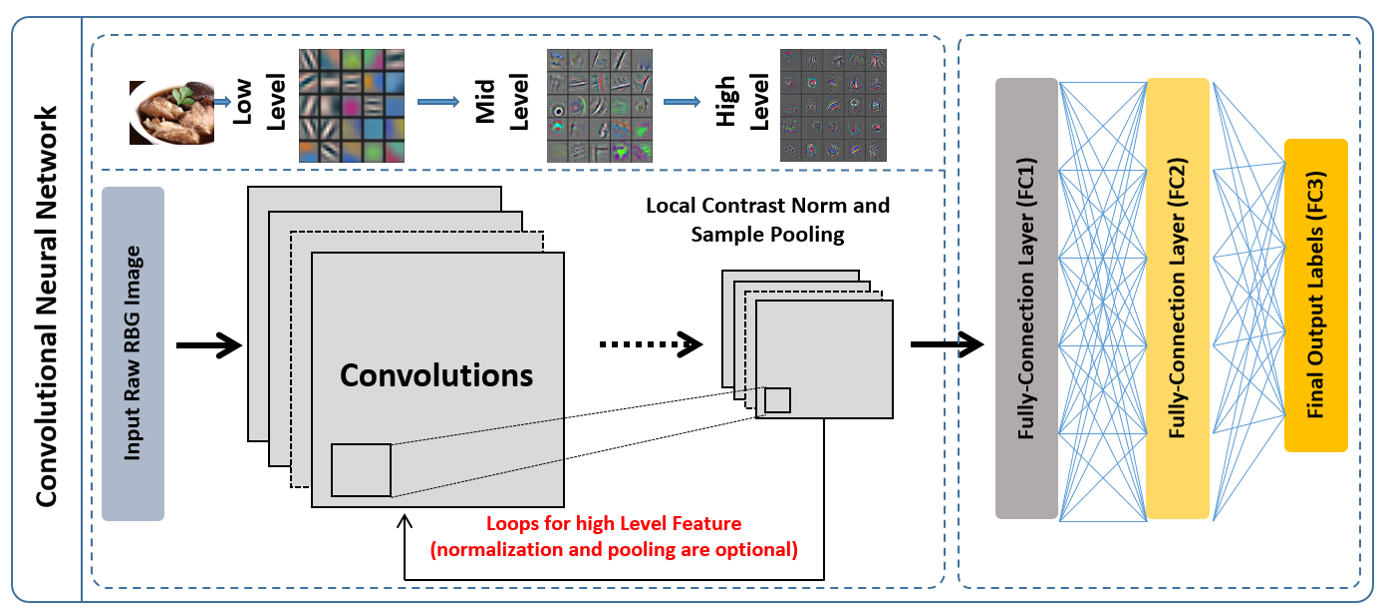
\includegraphics[clip=true, width=0.95\textwidth]{cnn.png}
    \caption{深度卷积神经网络的结构图}
    \label{fig:cnn}
\end{figure}

\subsection{经典卷积神经网络}
如图~\ref{fig:cnn}所示,经典深度卷积神经网络的前几层通常是卷积层,最后几层为全连接层,
不同的任务可能会采用不同深度的网络。最后一个全连接层的输出作为柔性最大传递函数(Softmax)
分类器的输入,得到在所有类别上的概率分布。假设训练数据为$X = [\x_1, \ldots,
\x_N]$,$\x_i$表示第i个图片, $N$是图片总数目。用$\y=[y_1, \ldots, y_N] \in
\R^{N}$表示训练数据的标注向量,$y_i \in [0,K-1]$是第i个图片的标注类别, $K$是类别数目。假设网络的层数为$M$,网络参数表示为
$W = \{W^1, \ldots, W^M\}, W^m \in \R^{d_{m-1}\times d_m}$。数据在第$m$层的特征图(Feature map)表示为
$Z^m(X) = [\z^m(\x_1), \ldots, \z^m(\x_N)]^T \in \R^{N \times d_m}$。

通常,卷积神经网络的损失函数是柔性最大传递函数的负对数似然函数和
权重衰减项(weight decay)之和:
\begin{equation}\label{eqn:cnn-loss}
    \L(W;X,\y) = -\frac{1}{N}\Big[\sum_{i=1}^N {\log p(y_i | \x_i; W)}\Big] + \frac{\beta}{2}\|W\|_F,
\end{equation}
其中,$\beta$是
权重衰减项的系数。上述损失函数相对于最后一层特征图$Z^M$以及参数$W^M$的梯度为:
\begin{eqnarray}
    Z^M &=& Z^{M-1}W^M \\
    \frac{\partial{\L(W;X,Y)}}{\partial{\z^M(\x_i)}} &=&
    -\frac{1}{N} \Big({\one_{y_i}(\z^M(\x_i)) - \p(\z^M(\x_i))}\Big) \\
    \frac{\partial{\L(W;X,Y)}}{\partial{W^M}} &=&
    (Z^{M-1})^T\frac{\partial{\L(W;X,Y)}}{\partial{\z^M(\x_i)}}\\
    &=& -\frac{1}{N}\sum_{i=1}^N {\z^{M-1}(x_i) \Big({\one_{y_i}(\z^M(\x_i))
    - \p(\z^M(\x_i))}\Big)^T}
\end{eqnarray}
其他层参数的梯度可以通过方向传播(Back
Propagation)得到~\cite{lecun1998gradient}。从上述公式可以看出,
错误的标注会导致参数梯度计算错误,并被反向传播, 使得经典的卷积神经网络
对于标注噪音十分敏感。

\subsection{相关反馈卷积神经网络}
目前已有部分工作研究弱监督深度学习, 然而现有方法大多基于特定的噪音模型,
难以处理真实的场景,或建模过于复杂,难以
训练。2014年谷歌研究团队提出的利用图片特征之间的相似性
监督网路学习,抑制错误标注影响的学习方法~\cite{reed2014training}。文章
认为,如果图片的特征之间具有相似性,那么预测的结果同样也应该比较类似,
并称之为感知连续性, 并将感知连续性应用到随机噪声假设下的网络学习中。本文
在感知连续性的基础上提出了不依赖于特定噪声类型的相关反馈卷积神经网络。

基于感知连续性,本文方法的基本假设是正确标注样本在图像空间具有相似性,
它们的特征表示在特征空间也具有相似性,而错误标注的样本则不具有这种相似性。
因此,可以利用特征之间的相关性作为反馈,
使得网络训练过程中不同数据在模型训练中发挥不同的作用。

为了表示特征之间的关系,我们将网络最后一层的特征转换为能反映
特征之间相互关系的关联特征表示(Affinity Representation)。类似于
Belkin等人提出的最近邻系统~\cite{belkin2001laplacian},我们定义如下
相似度矩阵$S\in R^{N \times N}$:
\begin{equation}\label{eqn:rf-cnn-sim}
    S_{ij} =
    \begin{cases}
        \exp\{-\frac{\|\z^M(\x_i) - \z^M(\x_j)\|^2}{\gamma^2}\} & y_i = y_j\\
        0 & \text{otherwise},
    \end{cases}
\end{equation}
$\gamma$是尺度因子。为了更好地反映相似度矩阵的局部结构,我们用一个对角矩阵$D$
对相似度矩阵进行正则化,$D_{ii} = \sum_{j=1}^N S_{ij}$。
训练数据最终的特征表示为$\Psi(X;W) = [\vpsi(\x_1), \ldots, \vpsi(\x_N)] =
D^{-1}S$,矩阵$\Psi(X;W)$的每一列包含了数据$\x_i$的特征和其他数据特征之间的关系。

假设理想情况下,不受噪音影响的模型参数为$W^*$,
则噪音鲁棒学习算法应该尽量优化$W$使其逼近$W^*$。
该优化目标可以通过最小化学习到的特征表示$\Psi(X;W)$和理想情况下的
特征表示$\Psi(X;W^*)$之间的差值$E_n$得到。$E_n$是由于噪音标注引起的特征表示的误差。
换句话说,可以认为$\Psi(X;W)$是理想特征与一个加性噪声之和:
\begin{equation}
    \Psi(X;W) = \Psi(X;W^*) + E_n
    \label{eqn:additive-noise}
\end{equation}
根据方程~\eqref{eqn:additive-noise}以及低秩理论~\cite{candes2011robust},
我们假设$\Psi(X;W^*)$是低秩矩阵:
\begin{equation}
    \text{rank}(\Psi(X;W)) > \text{rank}(\Psi(X;W^*))
\end{equation}

在社交多媒体数据上,假设类别数目足够多,
错误的标注来自于同一训练数据集上的其他类别, 并假定训练数据的特征最多有$K$个
模式,$\Psi(X;W^*)$的秩等于类别数目$K$,因此, $\Psi(X;
W^*)$可以通过如下优化方程得到:
\begin{eqnarray}
    \label{eqn:low-rank}
    \min_{\Psi(X;W^*)} \|\Psi(X;W) - \Psi(X;W^*)\|_F, \\ \nonumber
    \text{s.t.} \quad  \text{rank}(\Psi(X;W^*)) = K
\end{eqnarray}

\begin{figure}[ht]
    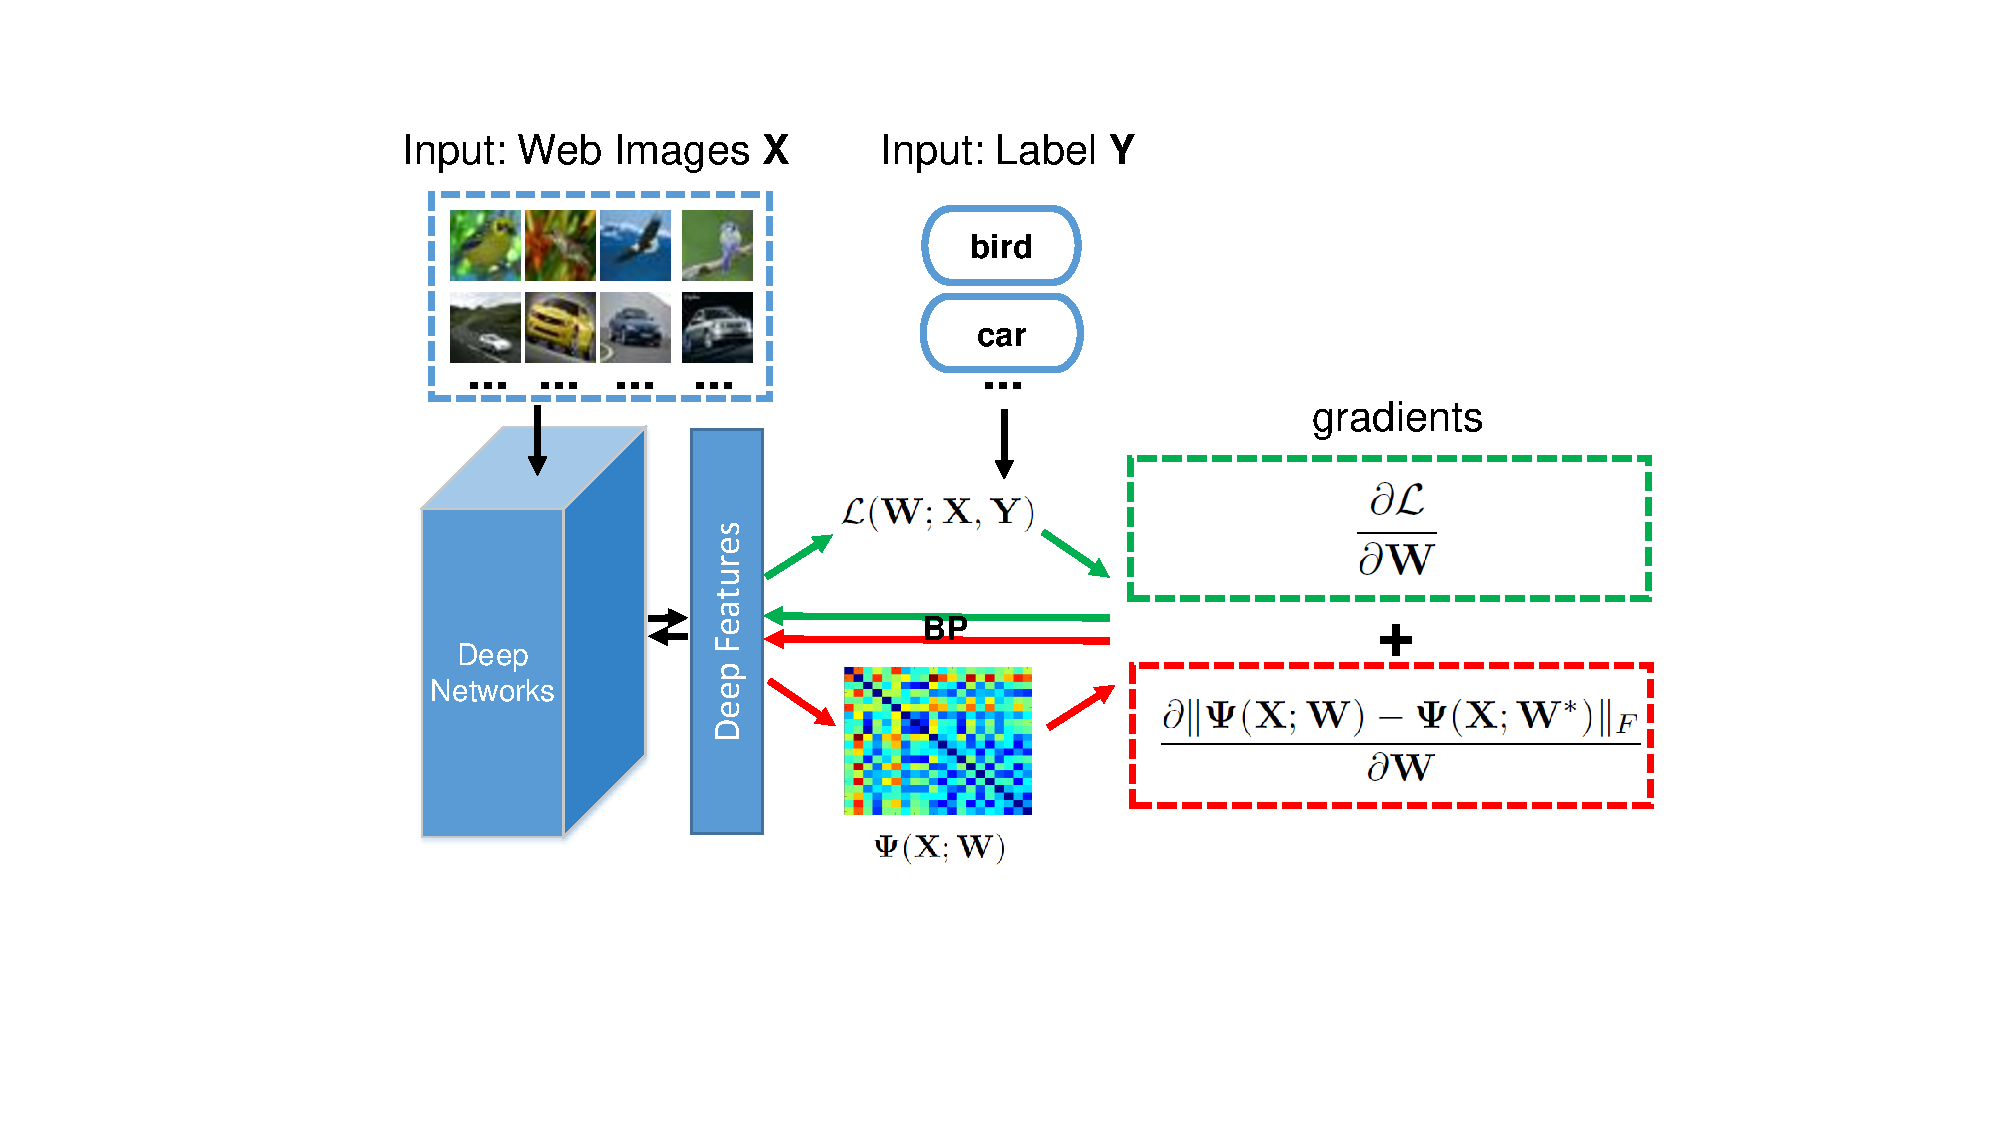
\includegraphics[clip=true, width=0.95\textwidth]{rf-cnn-frm}
    \caption{相关反馈卷积神经网络}\label{fig:rf-cnn-frm}
\end{figure}
如图~\ref{fig:rf-cnn-frm}所示,相关反馈卷积神经网络通过
特征矩阵的额重构误差,利用训练数据之间的感知连续性,
抑制训练过程中噪音的影响。
然而,由于方程~\eqref{eqn:low-rank}带来的计算量,
上述方法极大增加了优化过程的时间开销。此外,该方法优化过程分两步:
解优化方程~\eqref{eqn:low-rank}和反向传播。为了避免该方法呢的缺点,
本文进一步提出了改进的快速算法。快速算法基于下面的命题:
\begin{proposition}\label{prop:lowrank-spec}
    令$L=D-S, H^* \in R^{N\times K}$由$\Psi(X;W)$的K个最大的特征值
    对应的特征向量构成,可以得到:1)方程~\eqref{eqn:low-rank},即$\Psi(X;W)$
    的秩为$K$的最佳近似由特征向量矩阵$H^*$唯一决定;2)$H^*$也是下列优化方程的最优解:
    \begin{equation}
        \label{eqn:spec-cluster}
        \min_H \text{tr}[H^TLH] \quad \text{s.t.} \quad H^TH = I.
    \end{equation}
    由于方程~\eqref{eqn:low-rank}和方程~\eqref{eqn:spec-cluster}均在$H^*$取得
    最优值,可以认为方程~\eqref{eqn:low-rank}和方程~\eqref{eqn:spec-cluster}
    作为惩罚项是等价。
\end{proposition}
\begin{proof}
    命题~\ref{prop:lowrank-spec}可以通过如下三个定理得到。
    不失一般性,假设$\text{rank}(\Psi(X;W)) = r$。矩阵的秩为$K$
    的最小重构误差矩阵可以通过\emph{Eckart-Young-Mirsky}
    定理~\cite{eckart1936approximation}得到:
    \begin{theorem}[Eckart-Young-Mirsky]\label{thm:eym}
        对秩为$r$的矩阵$P\in \R^{m\times n}$进行奇异值分解(Singular Value
        Decomposition, SVD)得到$P=U\Sigma V^T, U^TU=I, V^TV=I$,
        如果$K < r$, 则有:
        $$%\begin{equation}
            \argmin_{
                \mbox{\scriptsize
                    $
                    \begin{array}{c}
                        \hat{P} \in \R^{m\times n} \\
                        \text{rank}(\hat{P}) = K
                    \end{array}
                    $
                }
            } \|P - \hat{P}\|_F = U\hat{\Sigma}V^T,
        $$%\end{equation}
        其中$\hat{\Sigma}$是包含$P$的前$K$个最大奇异值的对角矩阵。
    \end{theorem}

此外,如果矩阵$P$是实对称矩阵,它的奇异值和特征值之间具有如下定理所示关系:
\begin{theorem}\label{thm:evd}
    对实对称矩阵$P$特征值分解(EVD)得到$P=Q\Lambda Q^T, Q^TQ = I,
    \Lambda = \text{diag}(\lambda_1, \ldots, \lambda_N).
    \lambda_1 \geq \lambda_2 \geq \ldots \geq \lambda_N$是矩阵$P$的特征值。则有
    $$Q=U$$
\end{theorem}
因此,根据定理~\ref{thm:eym}和定理~\ref{thm:evd},实对称矩阵$\Psi(X;W)$的秩为$K$
的最小重构误差矩阵由$\Psi(X;W)$的前$K$个最大特征值对应的特征向量对应的矩阵构成。

根据Rayleigh~\cite{golub2012matrix}可以得到如下定理:
\begin{theorem}
    令$H^* = [\h_1^*, \ldots, \h_K^*] = \argmin_{H} \text{tr}[H^TLH]$,
    并且$H^TH = I$,
    则最优解$H^*$可以通过求解如下泛化特征值分解问题得到:
    $$
    L\h_i = (1-\lambda_i) D\h_i,
    $$
    其中$\{1-\lambda_i^* | i = 1,\ldots,
    K\}$是矩阵$\Psi(X;W)$的前K个最大特征值,
    $H^* = \{\h_i^* | i=1, \ldots, K\}$是对应的特征向量。
\end{theorem}
由于方程~\eqref{eqn:low-rank}和方程~\eqref{eqn:spec-cluster}均在$H^*$取得
最优值,可以认为方程~\eqref{eqn:low-rank}和方程~\eqref{eqn:spec-cluster}
作为惩罚项是等价。
\end{proof}

通过以上命题和证明可以发现,方程~\eqref{eqn:low-rank}的最优解可以通过
方程~\eqref{eqn:spec-cluster}中最小迹得到。因此,我们提出将最小迹的优化
目标引入到经典的神经网络中,最终的噪音鲁棒深度网络目标方程为:
\begin{equation}\label{eqn:rf-cnn-obj}
    \widetilde{\L} = \L(W;X,Y) + \alpha \text{tr}[H^TLH].
\end{equation}

上述优化方程仍然需要对特征矩阵进行特征值分解,本文提出了进一步的近似方法。
首先构建标注矩阵$Y = [\y_1,\ldots, \y_N]^T \in \{0,1\}^{N\times K}$, 每一列
$\y_i\in\{0,1\}^{K\times
1}$表示数据$\x_i$的标注向量,并且只有$y_i$位置为非零值。由于$Y$矩阵是在
语义空间上对数据的表述,$H$是在特征空间上的主成分表述,根据感知连续性,$H$
可以通过如下优化方程近似得到~\cite{yang2011l2,ye2008discriminative}:
\begin{equation}
    \min_{H} \|HH^T - YY^T\|_F^2.
\end{equation}
为了满足$H$矩阵的正交性,一个合理的近似解为$H = Y(Y^TY)^{-\frac{1}{2}}$。

\subsection{相关反馈分析}
为了验证上述方法有效性,我们从梯度的角度分析相关反馈对于噪声的抑制能力。
定义第$M$层特征之间的距离为:
\begin{eqnarray}
    \Delta(\x_i, \x_j) = \|\z^M(\x_i) - \z^M(\x_j)\|^2
\end{eqnarray}
当$y_i$与$y_j$相同时,$\x_i$和$\x_j$之间的距离$S_{ij}$表示为:
\begin{eqnarray}
    S_{ji}
    = \exp\{-\frac{\|\z^M(\x_j) - \z^M(\x_i)\|^2}{\gamma^2}\}
    = \exp\{-\frac{\Delta(\x_j, \x_i)}{\gamma^2}\}
\end{eqnarray}
$S_{ij}$相对于输入$\z^M(\x_i)$的梯度为:
\begin{eqnarray}
    \frac{\partial S_{ij}}{\partial \z^M(\x_i)} =
    \frac{\partial S_{ij}}{\partial \Delta(\x_i, \x_j)}
    \frac{\partial \Delta(\x_i, \x_j)}{\partial \z^M(\x_i)} =
    \frac{2S_{ij}}{\gamma^2}(\z^M(\x_i) - \z^M(\x_j))
\end{eqnarray}
定义$G=HH^T$,目标方程~\eqref{eqn:rf-cnn-obj}中的相关反馈项对于特征$\z^M(\x_i)$的梯度为:
\begin{eqnarray*}
    \frac{\partial tr(H^TLH)}{\partial \z^M(\x_i)} &=&
    \frac{\partial tr(HH^TL)}{\partial \z^M(\x_i)} =
    \frac{\partial tr(GL)}{\partial \z^M(\x_i)}
    =\frac{\sum_{k=1}^N\sum_{j=1}^N{G_{kj}\partial L_{jk}}}{\partial \z^M(\x_i)} \\
    &=&\frac{\sum_{k=1}^N\sum_{j=1}^N{(G_{kk} - G_{kj})\partial S_{kj}}}{\partial \z^M(\x_i)}  \\ 
    &=&\frac{2\sum_{k=1}^N\sum_{j=k+1}^N{(G_{kk} - G_{kj})\partial S_{kj}}}{\partial \z^M(\x_i)}  \\ 
    &=&\sum_{j=i+1}^N{(G_{ii} - G_{ij})}\frac{2\partial S_{ij}}{\partial \z^M(\x_i)}  \\ 
    &=&\sum_{j=i+1}^N{(G_{ii} - G_{ij})\frac{4S_{ij}}{\gamma^2}(\z^M(\x_i) - \z^M(\x_j))}  \\ 
    \|\frac{\partial tr(H^TLH)}{\partial \z^M(\x_i)}\|^2 &\propto&
    g(\Delta(\x_i, \x_j)) = \Delta(\x_i, \x_j)(\exp\{-\frac{\Delta(\x_i, \x_j)}{\gamma^2}\})^2
\end{eqnarray*}

图片$\x_i$对于梯度的贡献如图~\ref{fig:rf-cnn-gradient}所示的单峰函数。
在峰值的右边,随着$\x_i$和$\x_j$之间距离的增大,反馈的梯度逐渐减小至0,意味着
当同一类的样本直接距离过大时,相关反馈的作用较小。在峰值的左边,随着距离减小,
反馈的梯度也减小,距离为0时梯度也为0。这是因为深度学习需要多样化的训练样本,
距离为0意味着两个训练数据完全相同,反馈的梯度也应该为0。

\begin{figure}[ht]
    \center
    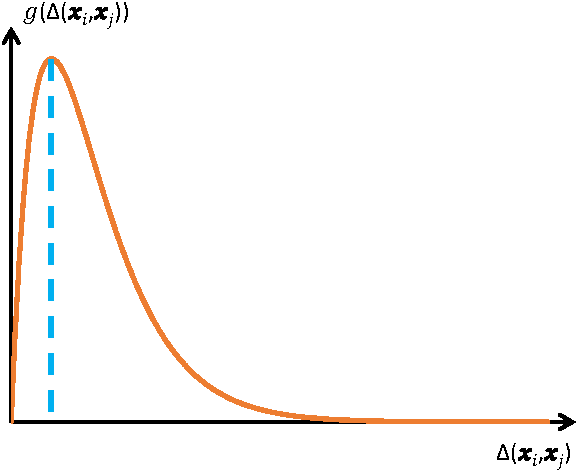
\includegraphics[clip=true, width=0.55\textwidth]{rf-cnn-gradient}
    \caption{训练数据对于梯度的贡献曲线,横坐标为数据与其他数据的距离}\label{fig:rf-cnn-gradient}
\end{figure}

\section{实验结果和评估}
本节从实验的角度验证本文提出的弱监督相关反馈卷积神经网络的有效性。
首先在标准数据集上验证该方法对于噪声标注的鲁棒性,其次,我们将该方法用于
真实的社交数据集,验证该方法在图片标注上的有效性。

\subsection{目标识别}

\textbf{实验数据}: 我们在两个公开数据集上分别验证算法对噪声的鲁棒性。
一个是CIFAR-10~\cite{krizhevsky2009learning},
包含$10$个类别$60,000$张$32\times 32$的彩色图片,其中
$50,000$用于训练,$10,000$用于测试。 为了产生不同噪声比例的训练数据,
在每个类别的训练数据上按照不同比例,随机选取图片,并将他们的类别随机替换为
数据集中的其他类别,训练数据集的总图片数目保持不变。在我们的实验设置中,
训练数据从无噪声到$90\%$的噪声均匀取$10$个噪声比例。
另一个数据集是PASCAL VOC2007~\cite{pascal-voc-2007},包含$20$个类别总共
$9,963$张图片。我们将数据集随机等分成训练数据和测试数据。

\textbf{比较基准}:本文提出的相关反馈卷积神经网络称为RFCNN,
并以下四个方法进行比较:
\begin{itemize}
    \item \textbf{CNN}: 经典的卷积神经网络。
    \item \textbf{RPCA+CNN}: 在训练卷积神经网络之前,首先用
        RPCA~\cite{candes2011robust}方法对每个训练数据进行重构,并移除重构误差较大的训练数据,
        移除的比例和噪音的比例相同。
    \item \textbf{CAE+CNN}:首先用卷积自动编码器对卷积神经网络的每一层
        进行预训练,然后微调整个网络,从而减小噪音标注的影响~\cite{luo2012hierarchical}。
    \item \textbf{NL+CNN}:用全连接层表示噪音转移概率矩阵,
        和卷积神经网络一起训练~\cite{sukhbaatar2014training}。
\end{itemize}

对于VOC2007数据集,我们还与另外两种方法进行比较:
\begin{itemize}
    \item \textbf{Best\_VOC}: 用ImageNet数据集预训练网络,
        并在VOC2007上微调~\cite{oquab2014learning}。
    \item \textbf{Web\_HOG}: 通过基于局部的模型和人工设计的特征,在网络图片上
        训练语义概念表征~\cite{divvala2014learning}。
\end{itemize}

\textbf{参数设置}:首先,我们调整公式~\eqref{eqn:cnn-loss}
中权重衰减项的系数$\beta$。对于$10\%$的噪音比例,该稀疏取$0.004$时
网路能达到最好的效果,对于$20\%$的噪音比例,取值为$0.008$,其他噪音比例下取值
为$0.04$。该参数设置对于两个数据集都能取得最好的效果。
此外,我们按照经验将公式~\eqref{eqn:rf-cnn-sim}中的$\gamma$参数设为$0.1$,使得特征相似度在合理的范围。
图~\ref{fig:rf-cnn-alpha}显示了在CIFAR-10数据集$20\%$噪音下,公式~\eqref{eqn:rf-cnn-obj}中不同$\alpha$取值
对于网络准确率的影响。我们发现,只有当$\alpha$取值过大时(比如取$10$),模型的
完全丧失了分类能力,对于其他取值,准确率都保持在相对稳定的范围,并在取值为$0.5$时
达到最优。此外,我们发现$\alpha$取$0.5$在其他噪音条件下也能取得最好的效果。因此,
以下实验$\alpha$均取$0.5$。
\begin{figure}[ht]
    \center
    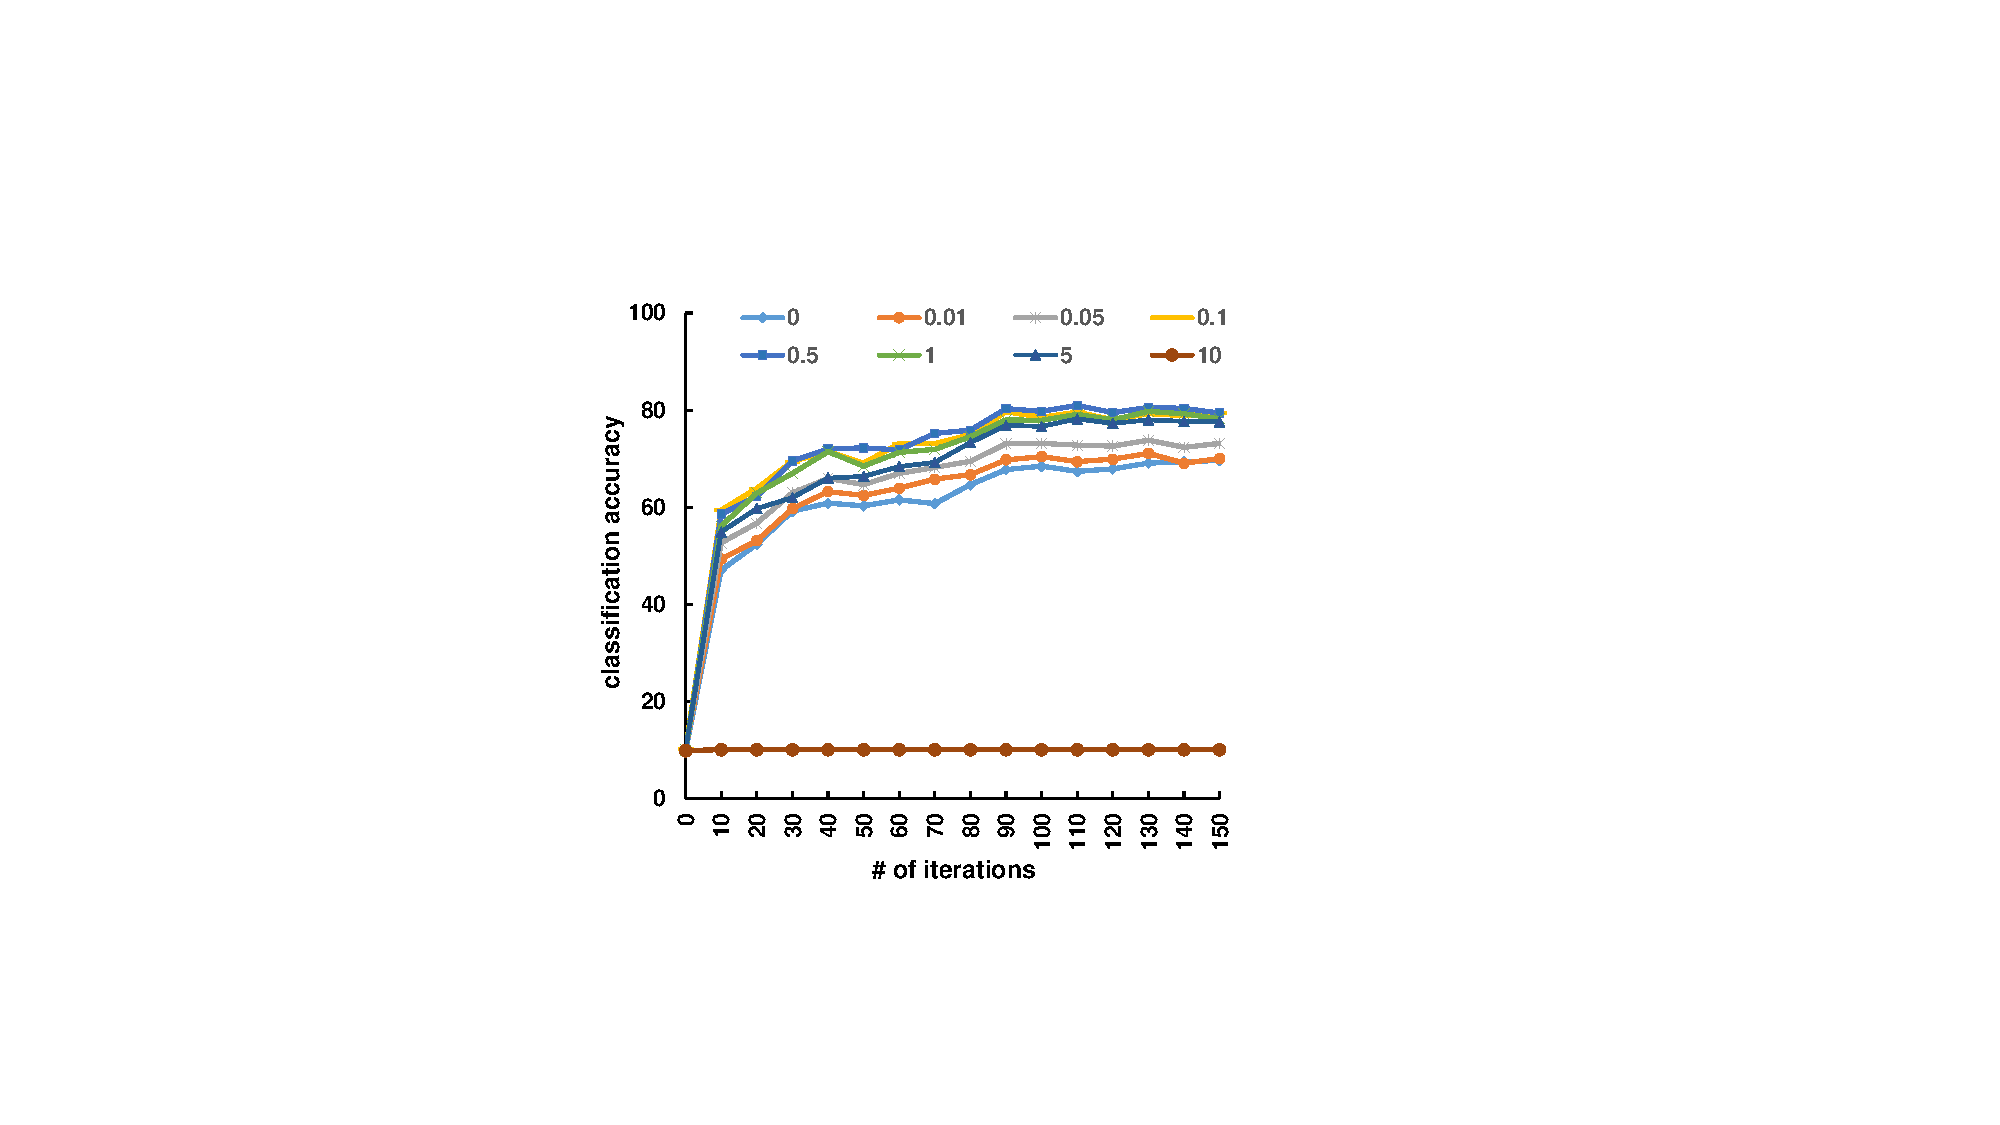
\includegraphics[clip=true, width=0.55\textwidth]{rf-cnn-alpha}
    \caption{参数$\alpha$对于卷积神经网络分类性能的影响}\label{fig:rf-cnn-alpha}
\end{figure}

\textbf{实验结果}:表格~\ref{tab:rf-cnn-cifar10}显示了在CIFAR-10数据集上不同噪音
程度下不同算法的分类准确率比较。本文提出的算法在所有条件下都达到了最好的实验结果,
甚至在无噪声数据集上,我们的算法也比经典的卷积神经网络取得了略好的准确率。我们发现,
在$30\%$噪音数据下,经典卷积神经网络的准确率下降了将近$20\%$。相比之下,本文提出的算法
值下降了$10\%$,表现出了对噪音数据很强的鲁棒性。此外,我们发现数据预处理方法RPCA+CNN在
噪音比例小于$50\%$时的准确率要好于经典的卷积神经网络,当有更多的噪音数据时,
RPCA+CNN的效果则比经典CNN要差。这个现象的原因在于当噪音数据增多时,
数据预处理移除正确数据的风险也随之增大,导致在最终的训练数据中噪音数据的比例增加。
CAE+CNN和NL+CNN算法的性能十分接近,在$30\%$噪音比例下,准确率分别下降$17.0\%$和
$15.9\%$。CAE+CNN虽然能够解决区域级的噪声(背景噪声),但对于样本集噪声(如本文中
的标注错误),它的鲁棒性则比较有限。对于NL+CNN,我们的实验证明仅仅在网路上增加一层
噪音适应层并不能噪音鲁棒性。相反,我们的方法可以抑制噪音在所有层的影响。
图~\ref{fig:rf-cnn-cifar-decline}反映了在不同噪音程度下不同方法分类准确率相对于
无噪声下降程度的比较。
\begin{figure}[ht]
    \center
    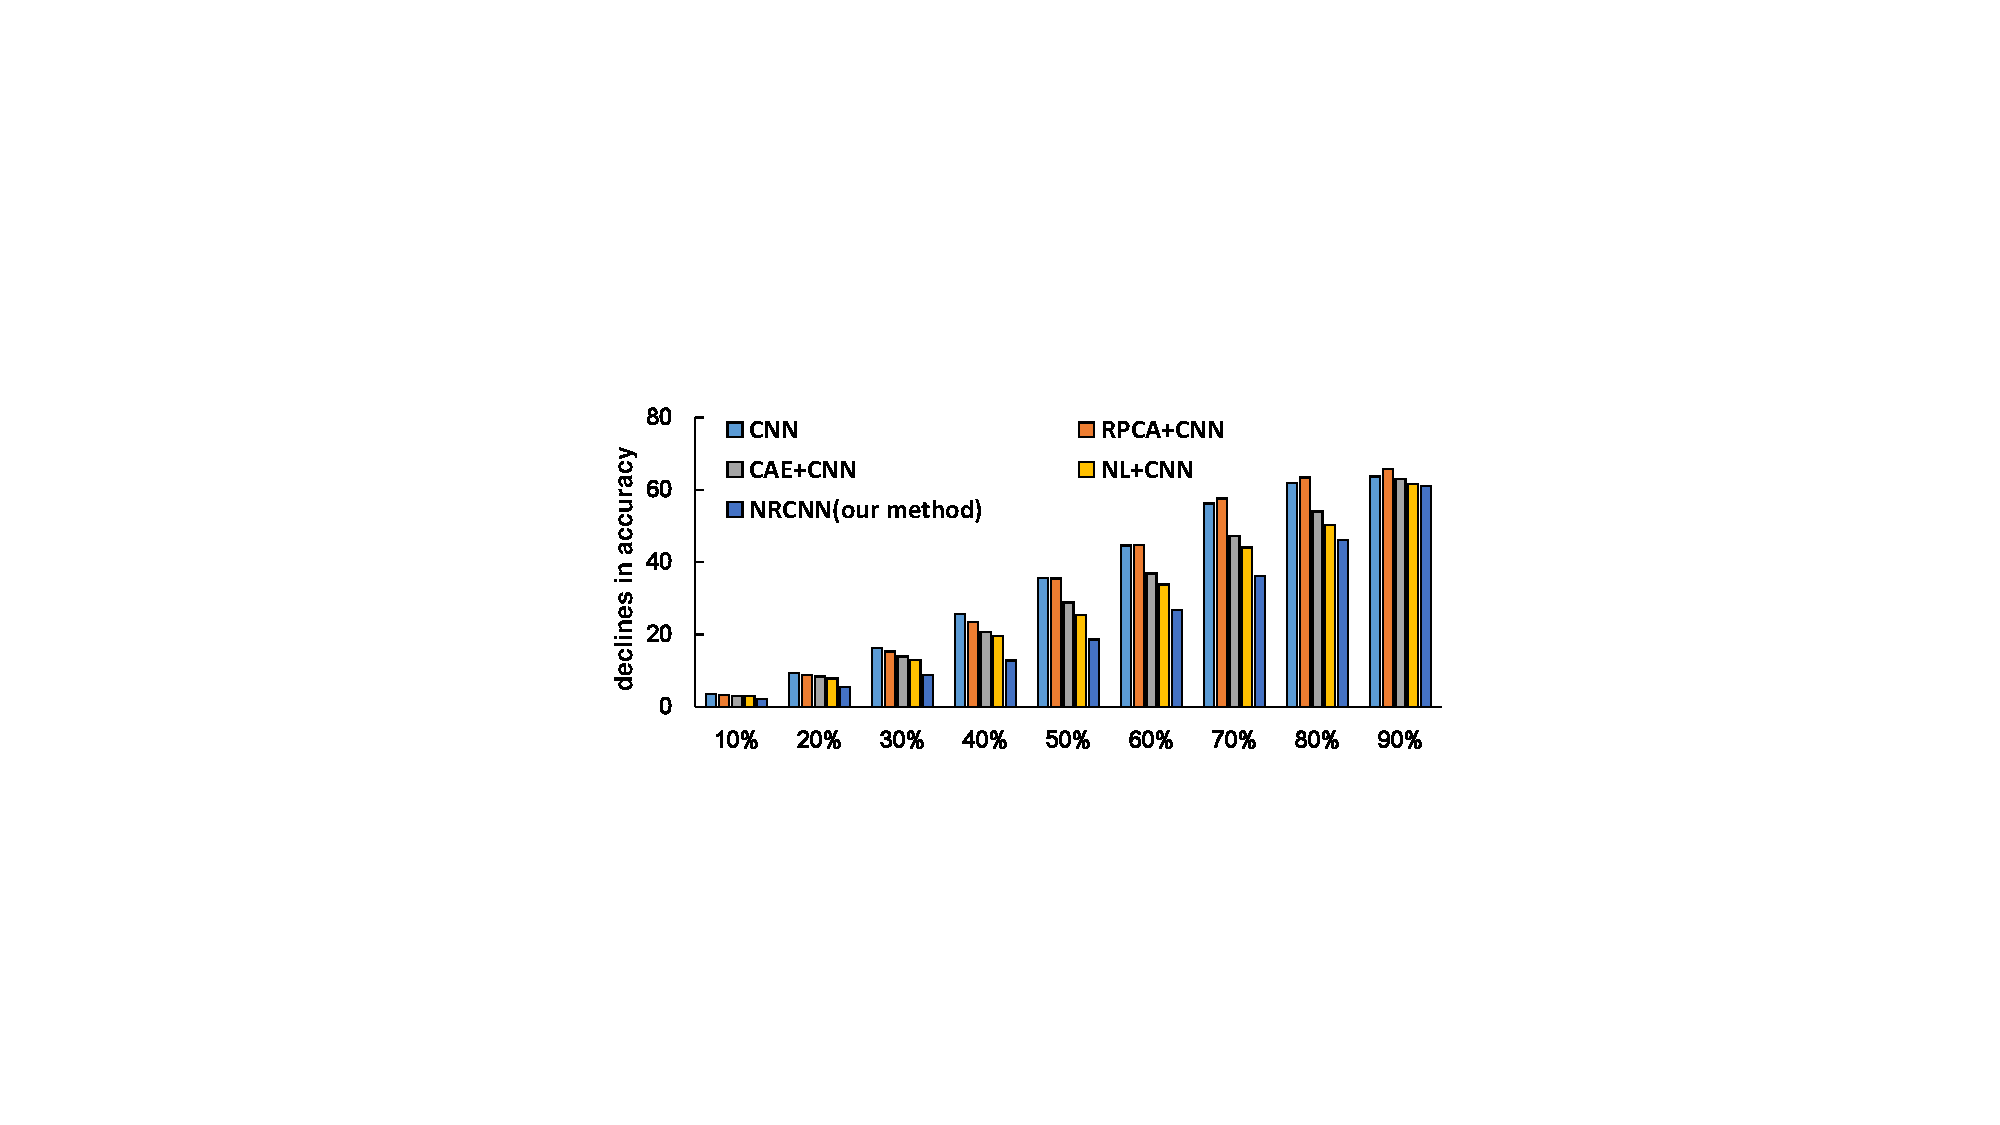
\includegraphics[clip=true, width=0.55\textwidth]{rf-cnn-cifar-decline}
    \caption{不同噪音程度下不同方法的准确率相对于无噪声的下降程度比较}
    \label{fig:rf-cnn-cifar-decline}
\end{figure}

\begin{table}[htbp]
    \centering
    \caption{不同算法在CIFAR-10数据集上不同噪音条件下的准确率比较}
    \label{tab:rf-cnn-cifar10}
    \small
    \begin{tabular}{|c|c|c|c|c|c|c|c|c|c|c|}
    \hline
    \diagbox{\scriptsize{算法}}{\scriptsize{噪声比例}} & 无噪声  & 10\% &  20\% & 30\% & 40\% & 50\% & 60\% & 70\% & 80\% & 90\% \\
    \hline
    CNN & 81.24 & 77.79 & 71.97 & 65.09 & 55.65 & 45.60 & 36.65 & 25.02 & 19.46 & 17.55 \\
    RPCA+CNN & 81.24 & 77.94 & 72.44 & 65.94 & 57.82 & 45.77 & 36.55 & 23.68 & 17.85 & 15.49\\
    CAE+CNN & 81.55 & 78.54 & 73.19 & 67.69 & 60.83 & 52.71 & 44.71 & 34.39 &
    27.54 & 18.61 \\
    NL+CNN & 81.16 & 78.28 & 73.36 & 68.26 & 61.63 & 55.83 & 47.33 & 37.12 &
    30.81 & 19.49 \\
    RFCNN & \textbf{81.60} & \textbf{79.39} & \textbf{76.21} & \textbf{72.81}
    & \textbf{68.79} & \textbf{63.01} & \textbf{54.78} & \textbf{45.48} &
    \textbf{35.43} & \textbf{20.56} \\
    \hline
\end{tabular}
\end{table}

在PASCAL VOC2007数据集上,我们使用AlexNet网络~\cite{krizhevsky2012imagenet}首先
在ImageNet数据集上预训练,然后在网络数据上微调网络参数。为了获取网络数据,
我们将数据集的每个类别作为查询词抓取搜索引擎的返回结果,并滤除重复的图片。
我们收集了两个训练数据集,第一个数据集中正负样本的数目和VOC2007中相同,
在该数据集上的实验我们记为CNN(Web)和RFCNN(Web)。第二个数据集中我们将正样本的
数目增加到VOC2007的4倍,并将该数据集上的方法记为CNN(Webx4)和RFCNN(Webx4)。
根据我们统计的结果,两个数据集上的噪音比例分别是$20\%$和$40\%$。不同方法
在VOC2007测试数据集上的平均准确率(Average Precision)如表~\ref{tab:rf-cnn-voc2007}所示。
可以发现:
\begin{itemize}
    \item
        CNN(Web)相比Web\_HOG具有十分明显的提升,证明了深度学习网络比利用人工设计的特征
        训练的分类模型具有更强的噪声鲁棒性。
    \item RFCNN(Webx4) 取得了比在大量标注好的数据集上训练的网络更好的效果。
\end{itemize}

\begin{table}[htbp]
    \centering
    \caption{不同算法在VOC2007数据集上不同噪音条件下的不同类别平均准确率比较}
    \label{tab:rf-cnn-voc2007}
    \footnotesize
    \tabcolsep=0.3mm
    \begin{tabular}{|c|c|c|c|c|c|c|c|c|c|c|c|c|c|c|c|c|c|c|c|c|c|}
    \hline
    \diagbox{\scriptsize{算法}}{\scriptsize{类别}} & plane  & bike & bird &
    boat & btl & bus & car & cat & chr & cow & tab & dog & horse & moto & pers
    & plnt & shp & sfa & train & tv & \textbf{mAP} \\
    \hline
    Best\_VOC & 88.5 & \textbf{81.5} & \textbf{87.9} & \textbf{82.0} & 47.5 &
    75.5 & \textbf{90.1} & 87.2 & 61.6 & 75.7 & \textbf{67.3} & 85.5 & 83.5 &
    80.0 & \textbf{95.6} & 60.8 & 76.8 & \textbf{58.0} & \textbf{90.4} &
    \textbf{77.9} & 77.7 \\
    Web\_HOG & 68.5 & 48.2 & 47.3 & 55.7 & 40.0 & 56.3 & 60.1 & 64.1 & 43.6 &
    59.2 & 32.9 & 46.5 & 56.2 & 62.4 & 41.3 & 29.6 & 41.4 & 35.6 & 68.9 & 35.5
    & 49.6 \\
    CNN(Web) & 84.1 & 68.8 & 77.1 & 73.0 & 63.0 & 74.2 & 74.3 & 79.2 & 61.8 &
    73.8 & 48.9 & 79.5 & 81.0 & 82.1 & 48.4 & 57.9 & 72.0 & 31.6 & 83.4 & 64.7
    & 68.9 \\
    CNN(Webx4) & 85.4 & 69.4 & 77.1 & 74.5 & 63.7 & 74.7 & 75.0 & 81.6 & 62.3 &
    75.7 & 53.3 & 80.2 & 83.8 & 84.6 & 50.7 & 58.9 & 75.9 & 41.0 & 84.5 & 69.1
    & 71.1 \\
    RFCNN(Web) & 85.8 & 69.7 & 77.4 & 75.1 & 63.8 & 75.8 & 75.6 & 82.7 & 62.7 &
    76.9 & 53.5 & 80.6 & 84.7 & 84.9 & 49.2 & 59.1 & 76.0 & 50.8 & 84.8 & 69.2
    & 71.9 \\
    RFCNN(Webx4) & \textbf{91.3} & 75.2 & 83.3 & 81.5 & \textbf{70.2} &
    \textbf{81.3} & 80.6 & \textbf{88.3} & \textbf{67.0} & \textbf{82.5} & 60.0
    & \textbf{86.3} & \textbf{90.0} & \textbf{90.3} & 75.8 & \textbf{64.8} &
    \textbf{81.0} & 57.8 & 89.9 & 74.9 & \textbf{78.6} \\ 
    \hline
\end{tabular}
\end{table}

\subsection{社交图片标注}
本章提出的相关反馈弱监督深度学习网路可以利用大量的社交图片作为训练数据,
用于任意类别的社交图片标注。例如,社交图片中广泛存在的``风景'',``家庭''标签并没有
相应的标注好的训练数据。

我们根据Flickr\footnote{\url{https://www.flickr.com/}}上$100,000$名活跃用户(注册
超过2年并在过去6个月上传超过500张找盘)提供的标签中选取了200个常见标签。其中50个标签例如
''日落'',''观光'',''生日''等没有在ImageNet数据集中出现。实验中的基准方法采用了ImageNet数据集。
对于这200个标签,我们仅用ImageNet数据集提供的每类$1,000$张图片作为训练数据训练模型,该方法称为\textbf{CNN(ImageNet)}。
此外,我们还采用了视觉语义嵌套方法DeViSE~\cite{frome2013devise},在150个已有训练数据类别上
训练视觉语义嵌套模型,从而对200个类别进行标注。
对于我们的方法,为了获得完整的200个类别的数据,我们从搜索引擎上为每个类别抓取$1,000$张图片,
移除重复图片并训练模型。网络模型与VOC2007实验中相同。

为了测试不同算法的性能,我们从\textbf{MIT-Adobe FiveK}数据集~\cite{fivek}中随即选取了
$1,000$张图片作为测试集。每种方法根据预测的分数为每张图生成5个有序标签。我们邀请了25位
标注人员为每个标签打分:2——非常相关;1——相关;0——不相关。我们采用归一化折扣增益值(NDCG)
作为评价指标。NDCG可以评价不同级别的相关性,相关结果越靠前得到的评分越高。有序结果中
位置$p$的NDCG定义为:
\begin{eqnarray}
    \text{NDCG}@p = Z_p \sum_{i=1}^p \frac{2^{r^i} - 1}{\log{(1+i)}}
\end{eqnarray}
其中$2^{r^i}$是第$i$个标签的相关性评价,$Z_p$是归一化参数。

表格~\ref{tab:rl-social-tagging-comp}显示了相关性评价结果。相比与其他噪音鲁棒算法,
本章提出的方法获得了最好的效果。此外,CNN(ImageNet)数据集由于训练的标注空间较小,
效果较差,从而证明了利用社交图片的有效性。
本章算法的效果也比视觉语义嵌套方法DeViSE要好。
\begin{table}[htbp]
\centering
\caption{社交图片标注结果比较} \label{tab:rl-social-tagging-comp}
\footnotesize
\tabcolsep=0.3mm
\begin{tabular}{|c|c|c|c|c|c|c|c|}
    \hline
    & CNN(Web) & RPCA+CNN(Web) & CAE+CNN(Web) & NL+CNN(Web) & CNN(ImageNet) &
    DeViSE(ImageNet) & RFCNN(Web)\\
    \hline
    NDCG@1 & 0.08 & 0.23 & 0.11 & 0.24 & 0.20 & 0.28 & \textbf{0.32}\\
    \hline
    NDCG@3 & 0.18 & 0.32 & 0.25 & 0.33 & 0.29 & 0.36 & \textbf{0.41}\\
    \hline
    NDCG@5 & 0.26 & 0.39 & 0.34 & 0.41 & 0.39 & 0.43 & \textbf{0.46}\\
    \hline
\end{tabular}
\end{table}

\section{小结}
本章提出了相关反馈弱监督深度学习网络,从大量的弱标注社交图片中学习物体识别模型。
算法可以在不需要人工标注的情况下快速学习任意的语义类别。算法利用了训练数据在之间的
相关性使得不同的训练数据在网络训练时有不同的梯度贡献。为了提高算法的效率,本文对
相关反馈弱监督神经网络进行了进一步的近似和简化。本章在标注数据集上混入噪声以及真实
的社交图片上验证算法的有效性。

本章的主要贡献包括:
\begin{itemize}
    \item 利用语义连续性提出了端到端的相关反馈弱监督神经网络,
        从社交图片中学习任意语义类别。
    \item 对相关反馈网路进行了简化近似,提高了算法的计算速度。
    \item 本文提出的相关反馈弱监督神经网络不依赖特定的网络结构。
\end{itemize}


\chapter{大规模社交多媒体数据快速处理}
社交多媒体数据由于规模庞大,需要耗费大量的计算资源和时间进行处理。本章主要从特征选取
和模型简化的角度讨论大规模社交多媒体数据的快速处理。

本章首先介绍用于大规模高维数据的特征选取算法。 对于社交多媒体数据的特征描述
不仅包括高层次的卷积神经网络特征,还包含低层次全局特征(如颜色特征,纹理特
征),局部特征(如SIFT,SURF)以及用来通过局部特征描述整体视觉信息的词袋特征等。实际应用
中需要根据需求选取对目标任务最有用的特征子集,这对于大规模社交多媒体数据的处理速度以及
移动设备有限的计算能力和内存空间尤其重要。此外,去除特定任务不相干的特征,还可以提高特
征的表达能力。

其次,本章介绍用于深度卷积神经网络的模型简化算法。
深度卷积神经网络在很多计算机视觉领域都表现出很好的性能,
然而网络的深度和模型参数通常比较大,例如经典的 VGG-16 网络包含超过200M的模型参数。
大量的模型参数意味着在实际应用中需要大量的计算资源和时间,极大地限制了深度神经网络
在大规模图片检索和图片识别等任务上的应用。此外,深度网络在移动设备上的应用已经成为一种
趋势。由于移动设备计算能力的限制,在不影响模型准确度的条件下简化深度网络模型已经成为迫
切的需要。

\section{二阶在线特征选取}
特征选取是指从数据中移除不相关或者冗余特征的过程。在当前大数据的背景下,特征选取
已经成为了十分重要的一项技术,并在多个领域尤其是高维数据的场景下获得了
广泛应用~\cite{Bolon015RAE,Zhai14EBD}。尽管特征选取已经被广泛的研究,大部分的算法
都属于批处理学习。批处理学习的主要问题在于它需要将整个数据集加载到内存中,由于计算机的
内存容量无法跟上数据规模,这对于实际问题中大规模高维数据显然不具有可伸缩性。此外,
批处理方法假设所有的训练数据和特征在训练前已经给定,而实际场景中需要处理的往往是流数据,
并可能伴随有新的特征出现。为了克服已有算法的这些问题,
近年来有部分工作研究在线特征选取~\cite{wang2014online,wu2010online,yang2013efficient}。
在线学习的优点在于算法每次迭代只处理一个数据,从而达到很高的可伸缩性,
并且可以很好地应对数据中模式和特征的变化。然而,目前已有的在线特征选取算法复杂度仍然过高,
模型的准确率与批处理方法也有不小差距。因此,文本提出了二阶在线特征选取算法,不仅对于
大规模高维数据具有很高的可伸缩性和学习效率,算法的准确率也与批处理方法十分接近。

不失一般性,我们首先研究二分类问题,并在~\ref{ssec:smofs}章节将算法扩展到多类问题。
令$\{(\x^t,y^t)|t=1,\ldots, T\}$表示训练过程中依次收到的数据,每个数据$\x^t
\in
\R^d$是一个$d$维的向量,数据类别$y^t\in\{+1,-1\}$。
在线学习算法将学习一个相同维度的分类器$\w \in \R^d$。
在时刻$t$,算法接收到数据$\x^t$,并基于当前的模型参数$\w^t$预测它的类别$\hat{y}\in\{+1,-1\}$。
\begin{equation}\label{eqn:predict}
    \hat{y}^t = \sign(\w^t \cdot \x^t)。
\end{equation}
预测完以后,算法将得到真实的类别$y^t$,从而衡量在数据$(\x^t,y^t)$上的损失函数$\ell(\w^t)$。
损失函数通常为真实类别和预测结果之间的差值的函数。在每轮迭代的最后,算法根据特定的规则更新
模型参数$\w^t$。例如,在线梯度下降算法更新的规则为:
\begin{equation}
    \w^{t+1} = \w^t + \eta^ty^t\x^t,
\end{equation}
$\eta^t$是时刻$t$的学习率(learning
rate)。根据不同的更新规则,在线学习算法可以分为两类:
\begin{itemize}
    \item 一阶算法:本质上是梯度下降算法~\cite{crammer2006online};
    \item 二阶算法:挖掘输入数据的几何特点~\cite{crammer2009adaptive}
        或构建目标方程的近似海森矩阵~\cite{duchi2011adaptive};
\end{itemize}
在线特征选取需要选取权重向量$\w^t$中相对较小的一部分元素,并将其他元素设为$0$。
换句话说,我们对$\w$的$L_0$范式施加如下约束:
\begin{equation}
    \|\w\|_0 \leq B, \|\w\|_0 = \sum_{i=1}^d w_i^0,
\end{equation}
$B$是预先定义的常数,因此,最多只有$\x$的$B$个特征被用来做预测。

\section{置信度加权二阶在线特征选取}
在线特征选取最直接的一种做法是运用截断感知机算法(Perceptron with
Truncation, PET)~\cite{wang2014online}。具体来说,分类器在每次迭代首先
根据$\w^t$预测类别$\hat{y}^t$。如果$\hat{y}^t$是正确的,则$\w^{t+1}=\w^t$;
否则,分类器根据感知机规则更新$\w^t$:$\hat{\w}^{t+1} = \w^t + \eta y^t\x^t$。
更新后的参数进一步被保留绝对值最大的$B$个元素,其他元素的值设为$0$.截断后的分类器参数
$\w^{t+1}$将被用于下一次迭代数据的预测。算法~\ref{alg:pet}显示了PET算法的框架,
算法~\ref{alg:truncate}显示了在线特征选取的截断函数。


\IncMargin{1em}
\begin{algorithm}
\SetKwData{Left}{left}\SetKwData{This}{this}\SetKwData{Up}{up}
\SetKwFunction{Union}{Union}\SetKwFunction{FindCompress}{FindCompress}
\SetKwInOut{Input}{input}\SetKwInOut{Output}{output}

\Input{$B$ - 需要选取的特征个数,$\eta$ - 学习率}
\Output{权重向量$\w^T$}
\BlankLine
初始化$\w^1 = \zero$\;
\For{$i\leftarrow 1$ \KwTo $T$}{
    接收到数据$\x^t\in \R^d$,预测类别$\hat{y}^t = \sign(\w^t\cdot \x^t$\;
    接收真实类别$y^t$\;
    计算损失函数$\ell(\w^t)$\;
    \If{$\ell(\w^t)>0$}{
        $\hat{\w}^{t+1} = \w^t + \eta y^t \x^t$\;
        $\w^{t+1} = \Truncate(\hat{\w}^{t+1},B)$\;
    }
}
\caption{PET:截断感知机算法框架}\label{alg:pet}
\end{algorithm}\DecMargin{1em}

\IncMargin{1em}
\begin{algorithm}
\SetKwData{Left}{left}\SetKwData{This}{this}\SetKwData{Up}{up}
\SetKwFunction{Union}{Union}\SetKwFunction{FindCompress}{FindCompress}
\SetKwInOut{Input}{input}\SetKwInOut{Output}{output}

\Input{$\hat{\w}$ - 权重向量,$B$ - 需要选取的特征个数}
\Output{截断的权重向量$\w$}
\BlankLine
$\w=\hat{\w}$\;
\If{$\|\hat{\w}\|_0 > B$}{
    除了$\w$的绝对值最大的$B$个元素,其他元素全部设为0\;
}
\caption{Truncate: 截断函数}\label{alg:truncate}
\end{algorithm}\DecMargin{1em}

根据Wang等人的分析,上述算法在实际应用中并不总能取得很好的效果。它不能保证被截断
的参数足够小,因而不能保证很小的错误率。因此,他们在截断之前运用稀疏投影,
提出了一阶在线特征提取算法(FOFS)。FOFS算法保证了每轮迭代分类器参数$\w^t$都限制在
一个$L_1$范式约束的超体内部。算法显示了FOFS算法的细节。

\IncMargin{1em}
\begin{algorithm}
\SetKwData{Left}{left}\SetKwData{This}{this}\SetKwData{Up}{up}
\SetKwFunction{Union}{Union}\SetKwFunction{FindCompress}{FindCompress}
\SetKwInOut{Input}{input}\SetKwInOut{Output}{output}

\Input{$B$ - 需要选取的特征个数,$\eta$ - 学习率,$\lambda$ - 正则化参数}
\Output{截断的权重向量$\w$}
\BlankLine
$\tilde{\w}^{t+1} = (1-\lambda\eta)\w^t + \eta y^t \x^t$\;
$\hat{\w}^{t+1} = \min\{1,\frac{\frac{1}{\sqrt{\lambda}}}{\|\tilde{\w}^{t+1}\|_2}\tilde{\w}^{t+1}\}$\;
$\w^{t+1} = \Truncate(\hat{\w}^{t+1}, B)$\;
\caption{FOFS:一阶在线特征选取算法}\label{alg:fofs}
\end{algorithm}\DecMargin{1em}

一般来说,一阶在线特征选取算法的复杂度和特征维度成正比。对于超高维度数据,
算法的速度会比较慢。此外,当输入数据的不同维度特征不在同一个尺度时,一阶算法
可能会移除有价值的特征。如公式~\eqref{eqn:predict}所示,预测结果不仅依赖于
权重向量,同时也依赖于输入数据。即使$|w_i|<|w_j|$,
并不能保证$w_i * E(x_i) < w_j * E(x_j)$,$E(x_i)$是$x_i$的期望。为了克服
一阶算法的局限性,我们探索了二阶在线学习最新发展,提出了二阶在线特征提取算法(SOFS)。

二阶置信度加权算法~\cite{dredze2008confidence}假设线性分类器的权重向量服从高斯分布
$\w\sim \Nn(\Mu, \Sigma)$。权重的置信度通过协方差矩阵$\Sigma$的对角元素表示,
对角元素$\Sigma_{jj}$越小,权重$\w_j$的均值的置信度越高。在观察到数据之前,
所有权重有共同的置信度或不确定性。在训练过程中,给定一个观察到的
训练数据$(\x^t,y^)$,置信度加权算法更新权重使得在当前数据$\x^t$上做出正确预测的
概率大于一个阈值$\tau$。同时,算法尽量保持与更新前的权重分布相同。置信度加权算法
可以表示为下面的优化问题:
\begin{eqnarray} \label{eqn:prob}
    (\hat{\Mu}^{t+1},\Sigma^{t+1}) &=&
    \argmin_{\Mu,\Sigma}{\DKL(\Nn(\Mu,\Sigma), \Nn(\Mu^t,\Sigma^t))}
    \nonumber \\
    s.t. &&\Pr_{\w\sim\Nn(\Mu,\Sigma)}[y^t(\w\cdot \x^t) \geq 0]  \geq \tau,
\end{eqnarray}
$\DKL(*,*)$是Kullback-Leibler(KL)距离。两个高斯分布$\Nn(\Mu,\Sigma)$和
$\Nn(\Mu^t,\Sigma^t)$的KL距离定义为:
\begin{eqnarray}
    \DKL(\Nn(\Mu,\Sigma), \Nn(\Mu^t,\Sigma^t)) &=&
    \frac{1}{2}\log{\frac{\text{det}\Sigma^t}{\text{det}\Sigma}}
    + \frac{1}{2}\text{Tr}((\Sigma^t)^{-1}\Sigma) \nonumber \\
    &+& \frac{1}{2}(\Mu^t - \Mu)^T(\Sigma^t)^{-1}(\Mu^t - \Mu) - \frac{d}{2}.
\end{eqnarray}
公式\eqref{eqn:prob}中的约束可以重新表达为:
$y^t(\Mu\cdot \x^t)  \geq  \phi\sqrt{(\x^t)^T\Sigma\x^t}$,
$\phi = \Phi^{-1}(\tau)$ ($\Phi)$是高斯分布的累积函数)。
研究人员提出了多种方法解公式~\eqref{eqn:prob}中的优化问题。本文
采用能够对每个训练数据的预测函数进行自适应正则化的AROW算法~\cite{crammer2009adaptive}。
研究和实验表明,该算法对于训练数据中的噪音具有更好的鲁棒性。
AROW算法的目标方程为:
\begin{eqnarray}
    (\hat{\Mu}^{t+1},\Sigma^{t+1}) =
    \argmin_{\Mu,\Sigma}\big\{\DKL(\Nn(\Mu,\Sigma),
    \Nn(\Mu^t,\Sigma^t))
    + \frac{1}{2\gamma}\ell^t(\Mu) + \frac{1}{2\gamma}(\x^t)^T\Sigma\x^t\big\},
    \label{eqn:arow_obj}
\end{eqnarray}
$\gamma > 0$是正则化参数。$\ell^t(\Mu)$是平方铰链损失函数:
\begin{eqnarray}
    \ell^t(\Mu) = \max(0,1 - y^t(\Mu \cdot \x^t))^2。
\end{eqnarray}

方程~\eqref{eqn:arow_obj}存在如下闭合解:
\begin{eqnarray}
    \label{equ:arow_solu}
    \beta^t &= \frac{1}{(\x^t)^T\Sigma^{t}\x^t + \gamma} \quad \g^t  =
    -2\max(0, 1 - y^t (\Mu^{t} \cdot \x^t) y^t\x^t \nonumber \\
    \hat{\Mu}^{t+1} &= \Mu^{t} - \frac{1}{2}\beta^t\Sigma^{t}\g^t \quad
    (\Sigma^{t+1})^{-1} = (\Sigma^t)^{-1} + \frac{\diag(\x^t(\x^t)^T)}{\gamma}
\end{eqnarray}

需要注意的是,本文提出的SOFS算法仅仅计算和考虑协方差矩阵$\Sigma$的对角元素。
从效率的角度,维持完整的协方差矩阵需要$O(d^2)$的内存空间和$O(d^2)$的计算复杂度,
这对于大规模超高维数据是不切实际的。从学习能力的角度,相关研究工作也表明在数据量
足够的情况下,对角协方差矩阵可以获得比完整协方差矩阵更好的性能,原因在于在学习初始
阶段完整协方差矩阵算法适应数据之间相互依赖的能力,当数据不可分时同业也使得它在逼近
最佳权重向量时过度拟合噪音~\cite{ma2010exploiting}。

不同于一阶在线特征选取算法基于权重向量的绝对值大小决定特征的重要性,本文提出的二阶在线
特征选取算法(SOFS)的核心思想是利用二阶信息保留B个置信度最高的特征。具体来说,在线学习
过程中,当在训练数据$(\x^t,y^t)$的损失函数不为$0$时,
我们仅更新前B个最小协方差$\Sigma_{jj}$对应的B个最确信的权重,剩余权重全部设为$0$。
算法显示了本文提出的SOFS算法框架。

\IncMargin{1em}
\begin{algorithm}
\SetKwData{Left}{left}\SetKwData{This}{this}\SetKwData{Up}{up}
\SetKwFunction{Union}{Union}\SetKwFunction{FindCompress}{FindCompress}
\SetKwInOut{Input}{input}\SetKwInOut{Output}{output}

\Input{$B$ - 需要选取的特征个数,$\gamma$ - 正则化参数}
\Output{权重向量$\Mu^T$和对角协方差矩阵$\Sigma^T$}
\BlankLine
初始化$\Mu^1=\one, \Sigma^1 = I$\;
\For{$i\leftarrow 1$ \KwTo $T$}{
    接收到数据$\x^t\in\R^d$,并预测$\hat{y}^t=\sign(\Mu^t\cdot\x^t)$\;
    接收到数据的真实类别$y^t$\;
    计算损失函数$\ell(\Mu^t)=\max(0,1-y^t(\Mu^t\cdot\x^t))^2$\;
    \If{$\ell(\Mu^t) > 0$} {
        根据公式~\eqref{equ:arow_solu}计算$\beta^t, \g^t$\;
        \For{$j\leftarrow 1$ \KwTo $d$}{
            $\hat{\mu}_j^{t+1} = \mu_j^t -
            \frac{1}{2}\beta^t\Sigma_{jj}^tg_j^t,
            (\Sigma_{jj}^{t+1})^{-1} = (\Sigma_{jj}^t)^{-1} +
            \frac{(x_j^t)^2}{\gamma}$\;
        }
        \For{$j\leftarrow 1$ \KwTo $d$}{
            \eIf{$\Sigma_{jj}^{t+1}$ 是最小的B个元素之一}{
                $\mu_j^{t+1} = \hat{\mu}_j^{t+1}$\;
            } {$\mu_j^{t+1}=0$\;}
        }
    }
}
\caption{二阶在线特征选取的算法框架}\label{alg:sofs}
\end{algorithm}\DecMargin{1em}

\section{二阶在线特征选取快速算法}
目前已有在线特征选取算法的一个普遍问题在于高计算复杂度。具体来说,
在线特征选取的一个主要时间开销在于从$d$维数组(FOFS算法中的权重绝对值向量和
SOFS算法中的最小B个元素)中选取最大会最小的$B$个元素。本文提出一个基于
最小堆的FOFS和PET算法的高效可伸缩方法,
用以替代在迭代的每一步对整个数组排序~\cite{wang2014online}。
此外,基于类似的最大堆的实现,我们利用SOFS算法的\emph{单调递减性}
进一步降低了SOFS算法的复杂度。

\subsection{一阶快速特征选取算法}
为了从$d$维数组中找出最大的$B$个元素
(算法~\ref{alg:truncate}中的Truncate函数),直接的做法是对$d$个元素排序,
然后选取前$B$个元素。为了提高计算效率,我们构建了一个最小堆用于存储权重向量
$\w^t$的$B$个最大绝对值。学习过程中,当分类器的权重向量发生改变时,
通过如下两步更新找出最大的$B$个元素:
\begin{itemize}
    \item 调整已经存在于堆中的元素的位置,维护最小堆结构。
    \item 比较不在堆中的每个元素与堆顶元素的大小。如果小于堆顶元素,
        则将它的值设为0,否则将堆顶元素替换为当前元素,并调整堆顶元素与子节点的
        位置,维护最小堆结构,原堆顶元素的值设为0。
\end{itemize}
算法~\ref{alg:fast-fofs}显示了改进的FOFS算法的详细步骤。
快速PET算法的过程与之类似。

\IncMargin{1em}
\begin{algorithm}
\SetKwData{Left}{left}\SetKwData{This}{this}\SetKwData{Up}{up}
\SetKwFunction{Union}{Union}\SetKwFunction{FindCompress}{FindCompress}
\SetKwInOut{Input}{input}\SetKwInOut{Output}{output}

\Input{$B$ - 需要选取的特征个数,$\eta$ - 学习率,$\lambda$ - 正则化参数}
\Output{权重向量$\Mu^T$}
\BlankLine
初始化$\w^1=\one, \v^1 = (|w^1_1|,\ldots,|w^1_d|) = \zero$,$\v^1$上大小为$B$的最小堆$H$\;
\For{$i\leftarrow 1$ \KwTo $T$}{
    接收到数据$\x^t\in\R^d$,并预测$\hat{y}^t=\sign(\w^t\cdot\x^t)$\;
    接收到数据的真实类别$y^t$\;
    计算损失函数$\ell(\w^t)$\;
    \If{$\ell(\w^t) > 0$} {
        $\Tilde{\w}^{t+1} = (1-\lambda\eta)\w^t + \eta y^t\x^t$\;
        $\w^{t+1} = \min\{1,\frac{\frac{1}{\sqrt{\lambda}}}{\|\Tilde{\w}^{t+1}\|_2}\}\Tilde{\w}^{t+1}$\;
        $\v^{t+1} = (|w^{t+1}_{1}|,\ldots,|w^{t+1}_{d}|)$\;
        调整$H$中节点的位置,维护最小堆结构\;
        \For{$j\leftarrow 1$ \KwTo $d, v_j^{t+1} \notin H$}{
            \eIf{$v_j^{t+1} > H_{min}$}{
                获取堆顶节点$H_{min}$,堆顶对应的特征位置记为$s$\;
                $w^{t+1}_{s} = 0$\;
                将堆顶$H_{min}$替换为$v^{t+1}_{j}$\;
                调整堆顶元素与子节点的位置,维护最小堆结构\;
            }{
                $w_j^{t+1} = 0$\;
            }
        }
    }
}
\caption{快速一阶在线特征选取算法}\label{alg:fast-fofs}
\end{algorithm}\DecMargin{1em}

为了说明上述算法的正确性,我们需要证明每次迭代以后绝对值最大的$B$个特征仍然在最小堆中。
用$h_1,\ldots, h_d$表示堆中特征的位置下标,其他不在堆中特征的下标为$h_{B+1},
\ldots, h_d$。在第一步中,$w_{h_1},\ldots, w_{h_B}$
被重新组织以满足最小堆的条件,我们有下面两个命题:
\begin{proposition}\label{prop:fofs1}
    如果模型更新后$w_{h_i}, \forall i \in [1,B]$仍然在最大的B个元素中,
    则$w_{h_i}$不会被替换出最小堆;
\end{proposition}
\begin{proposition}\label{prop:fofs2}
    如果模型更新后$w_{h_i}, \forall i \in (B,d]$在最大的B个元素中,
    则$w_{h_i}$一定会被替换进最小堆。
\end{proposition}
\begin{proof}
    对于命题~\ref{prop:fofs1},如果$w_{h_i}$不是$B$个最大元素中最小的,
    则$w_{h_i}$始终不会成为堆顶元素,因而一定不会被替换出最小堆。
    如果$w_{h_i}$是$B$个最大元素中最小的,
    则意味着最小堆中元素已经构成了最大的$B$个特征,
    剩下的$d-B$个特征权重的绝对值均比$w_{h_i}$小。
    因此仍然不会在第二步过程中被替换出最小堆。
    对于命题~\ref{prop:fofs2},我们可以得到$w_{h_i}$是最大的$B$个元素之一时,
    堆顶元素一定小于$w_{h_i}$,因此一定会被替换进最小堆。综上所述,
    本文提出的最小堆结构和更新方法可以找出权重绝对值最大的$B$个特征。
\end{proof}

\subsection{二阶快速特征选取算法}
尽管一阶快速特征选取算法已经避免了排序所有元素,
其算法复杂度依然和特征的维度成正比。
对于本文提出的二阶特征提取算法,
可以进一步利用二阶特征的特殊性将算法复杂度降低为和非零特征的个数成正比,
这对于大规模超高维度的稀疏数据具有重大的意义。区别于一阶在线特征选取算法,
本文提出的二阶算法具有如下单调递减特性:

\begin{proposition}[单调递减性]\label{prop:sofs}
    对于公式~\eqref{equ:arow_solu}中的对角协方差矩阵$\Sigma^t$,对于$\forall t$以及$\forall
    j\in[1,d]$,存在$\Sigma_{jj}^{t+1} \leq \Sigma_{jj}^t$。
\end{proposition}

命题的正确性可以由$\diag{(\x^t(\x^t)^T)}/\gamma$始终非负得到。基于上述命题,
本文提出二阶在线特征选取的的快速算法。
算法维护一个最大堆结构存储当前协方差矩阵的最小$B$个元素。
由于协方差矩阵每个元素的单调递减性质,对于每个被更新权重的特征,算法的更新规则为:
\begin{itemize}
    \item 如果特征已经在最大堆中,算法仅需要比较当前特征与子节点的大小,从而维护最大堆。
        因为置信度单调递减,更新后一定小于父节点;
    \item 如果被更新的特征不在最大堆中,则比较其与堆顶的大小,如果小于堆顶,则替换堆顶,
        并将原堆顶对应的特征权重置为$0$,否则将当前特征的权重置为$0$。
        对于没有被更新权重的特征,不需要进行比较,因为堆顶具有单调递减的特性,
        没有被更新权重的特征的置信度一定大于堆顶。
\end{itemize}
算法~\ref{alg:fast-sofs}显示了快速SOFS算法的细节。

\IncMargin{1em}
\begin{algorithm}
\SetKwData{Left}{left}\SetKwData{This}{this}\SetKwData{Up}{up}
\SetKwFunction{Union}{Union}\SetKwFunction{FindCompress}{FindCompress}
\SetKwInOut{Input}{input}\SetKwInOut{Output}{output}

\Input{$B$ - 需要选取的特征个数,$\gamma$ - 正则化参数}
\Output{权重向量$\Mu^T$和对角协方差矩阵$\Sigma^T$}
\BlankLine
初始化$\Mu^1=\one, \Sigma^1 = I$,$B$个$\Sigma^1$元素的最大堆$H$\;
\For{$i\leftarrow 1$ \KwTo $T$}{
    接收到数据$\x^t\in\R^d$,并预测$\hat{y}^t=\sign(\Mu^t\cdot\x^t)$\;
    接收到数据的真实类别$y^t$\;
    计算损失函数$\ell(\Mu^t)=\max(0,1-y^t(\Mu^t\cdot\x^t))^2$\;
    \If{$\ell(\Mu^t) > 0$} {
        根据公式~\eqref{equ:arow_solu}计算$\beta^t, \g^t$\;
        \For{$j\leftarrow 1$ \KwTo $d$}{
            $\hat{\mu}_j^{t+1} = \mu_j^t -
            \frac{1}{2}\beta^t\Sigma_{jj}^tg_j^t,
            (\Sigma_{jj}^{t+1})^{-1} = (\Sigma_{jj}^t)^{-1} +
            \frac{(x_j^t)^2}{\gamma}$\;
            \If{$\Sigma_{jj}^{t+1} \in H$}{
                递归调整$\Sigma_{jj}^{t+1}$与它子节点的位置,维护最大堆结构\;
            }
        }
        \For{$j\leftarrow 1$ \KwTo $d, x^t_j \neq 0, \Sigma_{jj}^{t+1} \notin H$}{
            \eIf{$\Sigma_{jj}^{t+1} < H_{max}$}{
                获取堆顶节点$H_{max}$,堆顶对应的特征位置记为$s$\;
                $\mu^{t+1}_{s} = 0$\;
                将堆顶$H_{max}$替换为$\Sigma^{t+1}_{jj}$\;
                调整堆顶元素与子节点的位置,维护最小堆结构\;
            }{
                $\mu_j^{t+1} = 0$\;
            }
        }
    }
}
\caption{SOFS:快速二阶在线特征选取算法}\label{alg:fast-sofs}
\end{algorithm}\DecMargin{1em}


\subsection{复杂度分析}
上述算法显著提高了在线特征选取的效率。本节分析上述算法的计算复杂度。

记权重向量的维度为$d$,每个数据平均非零特征个数为$m$,在最差情况下,PET算法每步
迭代需要的计算量为;
\begin{itemize}
    \item $2m$:计算损失函数,更新权重向量;
    \item $m$:计算权重向量的绝对值;
    \item $B\log B$:维护最小堆;
    \item $(d-B)\log B$:找出最大的$B$个元素,维护最小堆;
    \item $d-B$:将相应的特征值置为$0$.
\end{itemize}
PET算法每一步迭代的计算复杂度为$\{3m+d-B+d\log B\}$。

FOFS算法与PET算法类似,每步迭代需要:
\begin{itemize}
    \item $2m$:计算损失函数,更新模型;
    \item $d$:计算权重向量的范数;
    \item $d$:稀疏投影;
    \item $d$:计算权重向量的绝对向量;
    \item $B\log B$:维护最小堆;
    \item $(d-B)\log B$:找出最大的$B$个元素,维护最小堆;
    \item $d-B$:将相应的特征值向量置为$0$。
\end{itemize}
FOFS算法单步迭代的整体计算复杂度为$\{2m + 4d - B + d\log
B\}$,远高于PET算法。

SOFS算法迭代的复杂度为:
\begin{itemize}
    \item $3m$:计算损失函数,更新模型和对角协方差矩阵;
    \item $m\log B$:维护最大堆(只有$m$个值发生改变);
    \item $m$:将相应的特征值向量置为$0$。
\end{itemize}
SOFS算法迭代的复杂度降为$\{4m + m\log B\}$,当$m\ll d$并且$B\ll d$时,
SOFS算法处理大规模超高维度稀疏数据时具有很高的效率和可伸缩性。在最差情况下
$m\approx d$,SOFS算法复杂度与PET算法接近,但仍然小于FOFS。

对于空间复杂度,我们只考虑分类器需要的空间占用,不考虑数据加载和存储的内存开销。
在我们的实现中,输入数据存储成键值对的稀疏形式,处于效率考虑,模型参数表示成密集向量。
PET和FOFS算法要求保存权重向量$\w$和它的绝对值向量,因而空间复杂度为$O(2d)$。
SOFS算法也需要$O(2d)$的空间复杂度,用来保存权重向量和对角协方差矩阵。因此,
SOFS算法的空间复杂度和一阶在线特征选取算法的空间复杂度相同。

\section{二阶多类在线特征选取}\label{ssec:smofs}
多类问题中,假设共有$k$个类别,每个训练数据的类别为$y\in\{0,1,\ldots,k-1\}$。
我们采用一对多的策略(one-vs-the-rest)将二阶在线特征选取算法扩展到多类问题。
根据Crammer等人的策略~\cite{crammer2009multi},置信度加权模型的分布类似于二分类问题,
$\w\sim\Nn(\Mu,\Sigma), \Mu \in \R^{kd}, \Sigma\in\R^{kd\times
kd}$。我们引入新的类别相关的特征:
\begin{eqnarray*}
    \psi(\x,i) = [\zero^T,\ldots,\x^T,\ldots,\zero^T]^T,
\end{eqnarray*}
只有$\psi(\x,i)$的第i个位置为$\x$,其他位置为$\zero(\zero, \x \in \R^d)$。
在每次迭代中,分类器接收到训练数据$\x^t$并预测类别$\hat{y}^t =
\argmax_{i=0}^{k-1}{\Mu^t \cdot \psi(\x,i)}$。平方铰链损失函数为:
\begin{eqnarray}
    \ell(\Mu^t) = \max(0,1 - \Mu^t \cdot \Delta\psi^t)^2,
\end{eqnarray}
其中$\Delta\psi^t$依赖于多类问题更新的策略。
对于最大分数多分类更新:
\begin{eqnarray}
    \Delta\psi^t = \psi(\x^t,y^t) - \psi(\x^t,\argmax_{i=0,i \neq y^t}^{k-1}{\Mu^t
    \cdot \psi(\x,i))}
\end{eqnarray}
对于均匀多分类更新:
\begin{eqnarray}
    \Delta\psi^t &=& \sum_{i=0}^{k-1}\alpha^{t}_{i}\psi(\x^t,i), \quad
    \alpha^{t}_{i} =
    \begin{cases}
        -1 / |E^t|& i\in E^t\\
        1 & \text{if}\quad i = y^t\\
        0 & \text{otherwise}
    \end{cases}, \\
    E^t &=& \{i \neq y^t: \Mu^t \cdot \psi(\x^t, i)\geq \Mu^t \cdot \psi(\x^t,y^t)\},
\end{eqnarray}
多分类更新目标方程为:
\small
\begin{eqnarray}
    (\hat{\Mu}^{t+1},\Sigma^{t+1}) =
    \argmin_{\Mu,\Sigma}\big\{\DKL(\Nn(\Mu,\Sigma),
    \Nn(\Mu^t,\Sigma^t)) + \frac{1}{2\gamma}\ell(\Mu) +
    \frac{1}{2\gamma}(\Delta\psi^t)^T\Sigma\Delta\psi^t\big\}.
    \label{equ:multi_arow_obj}
\end{eqnarray}
\normalsize
目标方程的闭合解与公式~\eqref{equ:arow_solu}类似,区别在于将$y^t\x^t$替换成$\Delta\psi^t$。

我们仍然选取$B$个最确信特征。一对多策略的多类问题中,特征的置信度依赖于$k$个二分类器。
第$j$个特征的置信度定义为$C_j = k -
\sum_{i=0}^{k-1}\Sigma_{ij,ij}$。算法仅更新前$B$个最大$C_j$对应的权重参数,其他权重设为$0$。
算法细节与算法~\ref{alg:sofs}类似,区别在于将$y^t\x^t$替换成$\Delta\psi^t$。
多类SOFS算法的时间复杂度是二分类问题的$k$倍。

多类问题中$\sum_{i=0}^{k-1}\Sigma_{ij,ij}$仍然具有\emph{单调递减性}:
\begin{proposition}[单调递减性]
    对于公式~\eqref{equ:multi_arow_obj}中得到的$\Sigma^t$,对于$\forall
    t$和$\forall j \in [1,d]$,存在
    $\sum_{i=0}^{k-1}\Sigma^{t}_{ij,ij} \leq
    \sum_{i=0}^{k-1}\Sigma^{t+1}_{ij,ij}$。
\end{proposition}
因此,快速二分类二阶在线特征选取算法也适用于多类二阶在线特征选取。

\section{二阶在线特征选取实验评估}
本节在不同规模的人工数据和真实数据上用实验证明本文提出的二阶在线特征选取算法的有效性。

\subsection{实验设置}
对于在线特征选取算法,如果没有显式说明,我们仅在训练数据上学习一轮。我们比较本文提出的
算法和目前最好的在线和批处理特征选取算法,包括:
\begin{itemize}
    \item PET:截断感知机算法,在线特征选取的基准算法~\cite{wang2014online};
    \item FOFS:目前最好的一阶在线稀疏投影特征选取算法~\cite{wang2014online};
    \item mRMR: 最小冗余最大相关特征选取~\cite{peng2005feature},
        最好的批处理方法之一以及它的图形处理器并行版本(GPU-mRMR)~\cite{ramirez2016fast};
    \item Liblinear:用于大规模线性分类的开源库~\cite{fan2008liblinear},
        我们采用了其中的$l1-SVM$算法作为\emph{Embedded}特征选取的代表算法。 \item
        FGM:目前最好的批处理\emph{Embedded}特征选取方法之一~\cite{tantw14fgm}。
\end{itemize}

对于在线学习方法,我们使用铰链损失作为损失函数。我们使用五重交叉验证找出最优的超参数。
对于每一个数据集,在线学习方法随机打乱顺序$10$次并取平均训练结果作为最终结果。对于Liblinear
中的$l1-SVM$算法,我们调节$C$参数获得不同的特征个数。
对于FGM,为了简单起见我们遵循Tan等人论文中的设定将$C$设为$10$~\cite{tantw14fgm}。
对于mRMR,我们首先用它选取特定数目的特征,然后用在线梯度下降算法训练分类器。我们充分利用了
在线学习依次处理单个数据的特点,在实现中使用两个并行线程分别处理数据加载和模型训练。

\subsection{人工数据集实验评估}
我们仿照FGM算法的评估方法,人为产生了三种类型的人工合成数据,分别是$\X_1 \in
R^{100K\times 10K}, \X_2 \in R^{100K\times 20K}, \X_3 \in R^{1M\times1B}$,用来
测试算法的性能,效率以及可伸缩性。三个数据集都用于二分类任务。每个数据从独立同分布的
高斯分布$\Nn(0,1)$中采样得到。为了模拟真实的数据,每个采样得到的数据都是稀疏数据,
有效特征维度分别为$100$,$200$,和$500$。对于每一个数据,我们随机选取$\X_1$的$200$维,
$\X_2$的$400$维,和$\X_3$的$500$维作为噪声。为了获得数据的类别,我们从均匀高斯分布
$\Nn(0,1)$中采样得到权重向量$\w^*$作为正确的基准(groundtruth),每个数据类别为
$y=\sign(\w^*\cdot\x^*)$,$\x^*$是没有噪音特征的数据。合成数据集的详细情况如表~\ref{tab:synthetic-datasets}所示。

\begin{table}[htbp]
\caption{合成数据信息(``K'',``M'',``B''分别代表千,百万,十亿)}
\label{tab:synthetic-datasets}
\begin{center}
    \begin{minipage}{11cm}
        \begin{tabular}{|c|c|c|c|c|c|c|}
            \hline
            DataSet & \#Train & \#Test & Dim & IDim\footnote{有效特征维度} &
            NDim\footnote{噪音特征维度} & \#Feature \\
            \hline
            $X_1$ & 100K & 10K & 10K & 100 & 200 & 30M \\
            $X_2$ & 100K & 10K & 20K & 200 & 400 & 60M \\
            $X_3$ & 1M & 100K & 1B & 500 & 500 & 1B \\
            \hline
        \end{tabular}
    \end{minipage}
\end{center}
\end{table}

我们首先在$\X_1$和$\X_2$数据集上评估所有的特征选取算法。
$\X_3$数据集用来测试本文算法的效率和可伸缩性。
图~\ref{fig:synthetic-accuracy}和图~\ref{fig:synthetic-time}显示了
$\X_1$和$\X_2$上的准确率和时间开销。
\begin{figure}[t]
    \centerline{
        \subfigure[$\X_1$数据集]{ \includeMyGraphicX{synthetic-100k-fs-test-accuracy.pdf} }
        \subfigure[$\X_2$数据集]{ \includeMyGraphicX{synthetic-200k-fs-test-accuracy.pdf} }
    }
    \caption{合成数据集$X_1$和$X_2$上测试准确率和特征数目之间的关系}
    \label{fig:synthetic-accuracy}
\end{figure}

\textbf{准确率}。根据图~\ref{fig:synthetic-accuracy}中的结果,我们可以总结如下几点发现。
首先,当足够多有意义的特征被选取时($\X_1$中的100维,$\X_2$中的200维),SOFS算法可以达到
接近批处理特征选取算法的准确率,而且liblinear和FGM相对于SOFS算法的优势十分有限。
其次,当选取的特征数目较少时,批处理算法比在线学习算法更好。我们发现这种情况下
尤其是FGM和mRMR比在线学习算法要好很多。SOFS算法在特征不足是准确率不是很高,然而,
随着更多的特征被选取,它的准确率迅速饱和并达到最佳。再次,两个一阶在线特征选取算法
表现最差,尤其是在$\X_2$数据集上。仅在特征数目很少时PET和FOFS算法比SOFS算法准确率高。
然而,在特征数目足够多时,他们的性能不能达到与批处理算法相当的水平。总结起来,本文提出的
算法能有发掘出有意义的特征,并能在特征数目足够多的情况下达到类似于批处理算法的准确率。

\textbf{时间开销}。除了测试准确率,训练效率也是实际问题必须考虑的关键问题。图~\ref{fig:synthetic-time}
显示了各个算法的训练时间开销。一般来说,批处理算法虽然效果较好,但是时间开销远高于在线
学习算法。本文提出的SOFS算法只需要几秒钟就可以达到批处理相当的准确率。相反,liblinear需要
大约10倍的训练时间,FGM和mRMR在$\X_2$数据集上甚至需要100倍的训练时间。并行mRMR算法相对于
非并行算法减少了大约一半的时间。在线特征选取算法中,我们的方法仍然只需要最少的时间。我们发现
在这两个数据集上在线特征选取算法的时间开销差别不大,我们将在更大规模和更高维度上评估他们的区别。
尽管如此,准确率和时间开销的比较证明了SOFS算法是一个快速有效的在线特征选取算法。

\begin{figure}[t]
    \centerline{
    \subfigure[dataset $\X_1$]{ \includeMyGraphicX{synthetic-100k-fs-train-time.pdf} }
    \subfigure[dataset $\X_2$]{ \includeMyGraphicX{synthetic-200k-fs-train-time.pdf} }
    }
    \caption{Time cost versus number of selected features on synthetic datasets $\X_1$ and $\X_2$}
    \label{fig:synthetic-time}
\end{figure}

我们继而在大规模超高维度的$\X_3$数据集上测试SOFS的可伸缩性,由于已有特征选取算法在$\X_3$
上可能耗费几个小时甚至几天才能完成特征选取,我们仅在$\X_1$,$\X_2$和$\X_3$上测试SOFS算法是否
能够处理增长的维度和规模,特征选取的数目分别固定为$B=100,200,500$。此外,我们与两个
全特征维度上的在线学习基准算法比较,从而验证SOFS算法的有效性。两个基准算法分别是
在线梯度下降算法(OGD)和自适应权重向量正则化算法(AROW),结果如表~\ref{tab:sofs-scalability}所示。
\begin{table}[htbp]
\caption{SOFS算法可伸缩性评测}
\label{tab:sofs-scalability}
\begin{center}
    \begin{tabular}{|c|c|c|c|c|}
        \hline
        & Algorithm & $\X_1$ & $\X_2$ & $\X_3$  \\
        \hline
        \multirow{2}{*}{Time Cost} & OGD(s) & 3.58 & 7.06 & 114.82 \\
        & AROW(s) & 3.59 & 7.02 & 130.72 \\
        & SOFS(s) & \textbf{3.52} & \textbf{7.00} & \textbf{132.94} \\
        \hline
        \multirow{2}{*}{Accuracy} & OGD(\%) & 98.44 & 97.83 & 99.39 \\
        & AROW(\%) & 98.48 & 98.52 & 99.55 \\
        & SOFS(\%) & \textbf{99.17} & \textbf{98.62} & \textbf{99.56} \\
        \hline
        \multirow{2}{*}{Model Sparsity} & OGD(\%) & 0.00 & 0.00 & 83.16 \\
        & AROW(\%) & 0.00 & 0.00 & 72.22 \\
        & SOFS(\%) & \textbf{99.00} & \textbf{99.00} & \textbf{99.99} \\
        \hline
    \end{tabular}
\end{center}
\end{table}
根据表中的结果可以发现,测试准确率相对于基准算法有所提高,从而验证了移除不相关特征
可以提高模型效果。更重要的是,SOFS只需要少于$1\%$的特征就可以达到这个准确率。快速
有效的特征选取有如下三个好处:1)当输入特征是密集数据时,稀疏的分类器可以显著减少预测时间;
2)可以显著减少预测时的内存开销;3)可以显著减少特征提取的时间。在该数据集上,
OGD和AROW算法需要大约1GB内存存储分类器(每个权重需要4个字节),而SOFS算法仅需要
2KB。在嵌入式系统等内存空间十分有限的条件下,紧凑的分类器更加具有实际意义和经济价值。

此外,我们可以发现随着数据数目和特征维度的增加,SOFS的训练时间的增加在可接受的范围。
在十亿个特征的数据集上,它仅需要2分钟多的时间就可以完成模型训练和特征选取。相反,其他特征
选取算法陷入\emph{维度灾难}的问题。
例如,PET算法需要至少10个小时从$\X_3$中选取500个特征,更不用说其他风复杂的算法。此外,
我们特别注意到相比于基准在线学习算法的时间开销,SOFS并没有引入过多额外的时间开销。原因在于
在我们的实现中数据加载和模型训练分为两个线程同时进行,由于三个算法都比较高效,数据加载
实际上占据了主要的时间。总结起来,实验中的低训练时间和高准确率表明本文提出的算法
能够快速有效地挖掘大规模超高维度数据中的有效特征。
的

\subsection{大规模真实数据集实验评估}

\begin{table}[htbp]
    \centering
    \caption{大规模真实数据集信息}
    \label{tbl:sofs-large-datasets}
    \begin{tabular}{|c|c|c|c|c|}
        \hline
        数据集 & 特征维度 & 训练数据个数 & 测试数据个数 & 特征个数 \\
        \hline
        news & 1,355,191 & 10,000  & 9,996  & 5,513,533 \\
        rcv1 & 47,152 & 781,265 & 23,149 & 59,155,144 \\
        url & 3,231,961 & 2,000,000    & 396,130 & 231,249,028\\
        \hline
    \end{tabular}
\end{table}
本节在大规模真实数据集上评测SOFS算法的性能,采用的数据集如表~\ref{tbl:sofs-large-datasets}所示。
第一个数据集``news''维度较高,第二个数据集``rcv1''规模较大,第三个数据集``url''规模和维度
均较大。在本实验中为了简单起见,我们仅比较SOFS算法,PET算法(快速),FGM算法(高效)之间的差异。

\begin{figure}
    \centerline{
    \subfigure[news]{ \includeMyGraphicX{news-fs-test-accuracy.pdf} }
    \subfigure[rcv1]{ \includeMyGraphicX{rcv1-fs-test-accuracy.pdf} }
    }
    \centerline{
    \subfigure[news]{ \includeMyGraphicX{news-fs-train-time.pdf} }
    \subfigure[rcv1]{ \includeMyGraphicX{rcv1-fs-train-time.pdf} }
    }
    \caption{``news''和``rcv1''数据集上测试准确率和训练时间与选取特征个数之间的关系}
    \label{fig:sofs-comp-big}
\end{figure}

\begin{table}[htpb]
    \centering
    \caption{大规模高维数据集评测结果($\rho$ 是选取的特征比例)}
    \label{tbl:sofs-comp-big}
    \footnotesize
    %\tabcolsep=0.6mm
    \begin{tabular}{|c|c|c|c|c|c|}
        \hline
        Dataset & $\rho$ & 0.005 & 0.05 & 0.1 & 0.2\\\hline
        \multirow{3}{*}{news}& PET & 90.33$\%$(41.34s) & 94.09$\%$(32.18s) &
        93.91$\%$(36.54s) & 95.08$\%$(31.37s) \\
        &SOFS &  91.26$\%$(\textbf{0.61s}) & 94.76$\%$(\textbf{0.63s})  &
        95.33$\%$(\textbf{0.60s})  & \textbf{95.84}$\%$(\textbf{0.61s})\\
        &FGM  & \textbf{94.92}$\%$(90.10s)&
        \textbf{95.43}$\%$(1610.53s) & \textbf{95.47}$\%$(5206.20s) &
        95.46$\%$(15055.28s)\\\hline
        \multirow{3}{*}{rcv1} & PET & 73.18$\%$(79.13s)& 96.21$\%$(20.30s)&
        97.01$\%$(18.53s) & 97.37$\%$(24.63s)\\
        &SOFS & 90.40$\%$(\textbf{6.29s}) & 96.86$\%$(\textbf{6.27s}) &
        97.19$\%$(\textbf{6.28s}) & \textbf{97.65}$\%$(\textbf{6.32s})\\
        &FGM & \textbf{91.74}$\%$(394.98s)&
        \textbf{97.13}$\%$(1346.03s) & \textbf{97.37}$\%$(1994.78s)&
        97.54$\%$(3253.97s)\\\hline
        \multirow{2}{*}{url} & PET &  98.15$\%$(1100.28s)& 98.38$\%$(1664.15s) &
        98.21$\%$(1528.01s) &	98.21$\%$(1573.35s)\\
        &SOFS & \textbf{98.32}$\%$(\textbf{6.95s})  & \textbf{98.74}$\%$(\textbf{7.05s}) &
        \textbf{98.92}$\%$(\textbf{6.94s}) & \textbf{99.18}$\%$(\textbf{6.94s}) \\
        \hline
    \end{tabular}
\end{table}
表~\ref{tbl:sofs-comp-big}和图~\ref{fig:sofs-comp-big}显示了三个算法测试准确度和训练时间之间的比较结果。
由于FGM算法在``url''数据集上训练时间过久,因此表格中缺少相关实验结果。根据表格结果,我们可以
发现SOFS的性能十分接近甚至要优于FGM,尤其是当更多的特征被选取的时候。SOFS和FGM算法都比
基准算法PET要好。对于训练时间,PET和SOFS在``news''数据集上的比较结果表明PET对于维度更敏感。
一个有趣的现象在于PET算法在选取$0.5\%$的特征时需要耗费更多的时间,原因在于此时PET算法
收敛的速度过慢,需要反复地更新模型。FGM算法是计算做复杂的特征选取算法,训练时间通常比
在线特征选取算法高一个量级。此外,训练时间随着选取特征数目的增加也迅速增加。根据实验结果,
我们可以发现SOFS算法在大规模高维数据集上进行特征选取的巨大优势。在某些实际问题中,往往需要
在同一个数据集上反复运行多次在线算法使得模型收敛,此时SOFS算法的优势将更加明显。

\subsection{图片检索中的应用}
\section{深度卷积神经网络模型简化}
\subsection{深度卷积网络模型简化建模}
\subsection{基于在线学习的模型简化}
\subsection{实验结果和评估}
\section{小结}

\chapter{基于主题的照片集故事化表达}
随着只能手机和数码摄像头的增长,人们几乎可以在任何时间任何地点拍摄照片。
大部分被拍摄的照片仅仅被存储在云端,用户很少进一步接触这部分数据,
原因在于我们缺少只能的服务去组织用户数据。因此,当前急需相关的技术和系统
将用户静态的照片总结整理成故事,使得用户能够重现社交多媒体数据中的经典时刻。
本文提出了一个基于主题的照片集故事化系统Monet,在预先定义的编辑风格上模仿
电影剪辑的手法从个人照片集中生成故事化的表达视频。该系统包含两个阶段:
照片集总结阶段从照片集中选取一部分关键照片代表整个照片集,
以及故事合成阶段用选取的照片按照主题风格生成音乐视频。在照片集总结过程中,
照片根据时间和位置信息被划分到不同的事件,再根据照片的视觉质量,所在事件的代表性,
多样性选取一部分子集作为关键性照片。第二个阶段故事合成自动根据照片的内容选取合适的
基于主题的编辑风格。每张被选取的照片通过选取合适的相机运动被转换为视频片段。然后根据
电影编辑规则将一系列的视频特效,颜色过滤器,形状和转场效果附加到视频片段中。最终的视频
和音乐混流生成故事化的音乐视频。通过实验验证,
本文提出的系统达到了比当前最好的照片集时间检测和故事合成系统更好的效果。

\section{照片集故事化表达系统框架}
从照片集中产生有吸引力和纪念意义的故事化表达面临一些挑战。首先,海量的用户照片集通常
是无序的,使得照片的浏览和分享十分枯燥。然而,照片一般来说不是随机拍摄的,而是拍摄在
不同的事件的特殊时刻。对于故事化表达来说,能够将照片组织成时间变得异常必要。
其次,由于大部分用户没有专业的拍摄技术,很多用户照片存在质量较差和内容冗余的问题。
因此,从照片集中选取一部分有代表性的子集是照片集故事化表达的关键步骤。
再次,我们需要将选取的照片用有吸引力的方式重新呈现给用户,提升用户体验。
在我们的系统中,照片集通过音乐视频的方式表达。由于照片拍摄在不同的场景,系统
需要自动选取合适的编辑风格达到的不同的表达效果。
最后,为了增加音乐视频的吸引力,
应该在视频渲染时引入视频编辑元素,如特效,形状,颜色过滤器,转场等。
从专业的视频编辑的角度,这些编辑元素依赖特定的内容和风格。因此,如何挖掘视频编辑语法,
设计基于风格的编辑元素,并将它们运用到系统中是一项具有很大挑战性但又十分必要的部分。

本文提出的基于主题的照片集故事化系统如图~\ref{fig:monet-framework}所示。用户照片首先被
组织到不同的事件中,然后在事件中选取一部分关键照片作为对照片集内容的总结。
在选取的关键照片上,系统自动为它们选取合适的编辑风格。根据预先定义的编辑语法,
系统结合相机运动,视频特效和音乐产生视频片段。最后,通过在视频片段之间添加转场效果产生
完整的音乐视频。系统实现的细节将在后续章节逐一介绍。
\begin{figure}[ht]
    \center
    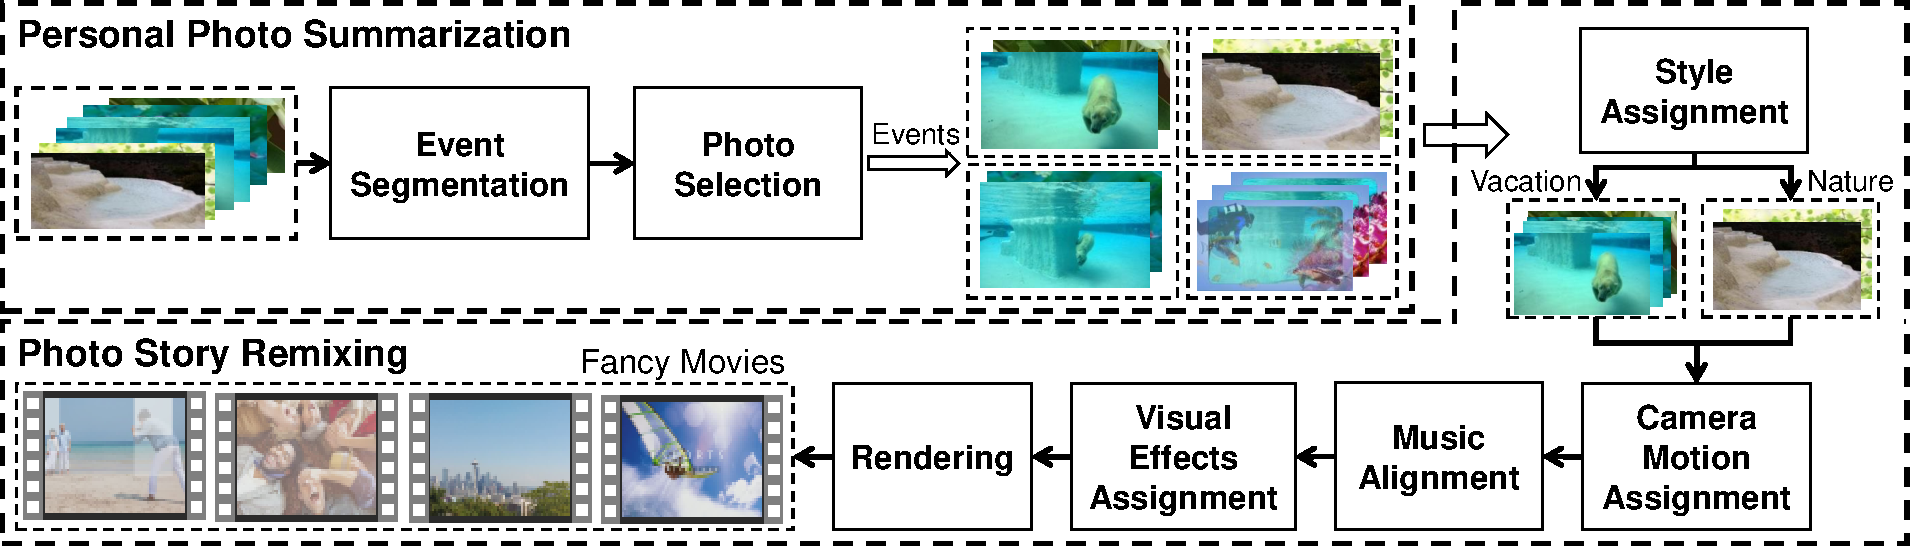
\includegraphics[clip=true, width=0.95\textwidth]{monet-framework.pdf}
    \caption{基于主题的照片集故事化表达系统框架}
    \label{fig:monet-framework}
\end{figure}

\section{照片集总结}
照片集总结包含两个步骤:事件检测和照片筛选。事件检测将照片按照事件进行组织。
照片筛选首先移除低质量或者重复的照片,然后选取高质量,有代表性,能够体现事件
均衡性的照片子集作为关键照片。

\subsection{事件检测}
从统计上来看,人们倾向于在集中的时间点拍摄照片。为了清楚地解释事件检测的概念,本文定义
``事件''如下:
\begin{definition}[\textbf{事件}]
    事件是特定的情景下、相对较短的时间段内, 用户记录值得留念的时刻的一组拍摄行为。
\end{definition}
因此,同一事件中的照片在时间和地点上比较接近。每个照片$\x_i \in \X = \{\x_1, \x_2,
\ldots, \x_N\}$属于事件$e_j \in E = \{e_1, e_2, \ldots,
e_K\}$,$N$和$K$分别是照片集$\X$中照片和事件的数目。相应地,照片$\x_i$属于事件$e_j$
的概率可以表示为$p(\x_i|e_j)$,$\x_i=(x_{i,1},
x_{i,2})$,$x_{i,1}$是时间($\mathcal{T}$),
$x_{i,2}$是GPS($\mathcal{G}$)。如果$p(e_j|x_i)$是最大的后验概率,则$x_i$被判定为
属于事件$e_j$。

给定事件$e_j$,假设时间和位置信息之间是相互独立的,似然函数$p(x_i|e_j)$被表示为:
\begin{equation}
    \label{equ:monet-priori}
    p(\x_i|e_j)= \prod_{l=1}^{2}p(x_{i,l}|e_j) = p(\mathcal{T}_i | e_j)p(\mathcal{G}_i | e_j).
\end{equation}
每个$x_{i,l}$相对于事件$e_j$的概率服从高斯分布:
\begin{equation}
    p(x_{i,l}|e_j) =
    \frac{1}{\sqrt{2\pi\delta_{j,l}^2}}e^{-\frac{(x_{i,l}-\mu_{j,l})^2}{2\delta_{j,l}^2}}.
\end{equation}
获得每个事件的分布的过程其实是学习混合高斯模型(GMM)的模型参数的过程$\Theta=\{\delta_{j,l},
\mu_{j,l}\}$。我们最大化如下目标方程所示的联合概率的对数似然函数:
\begin{equation}
    \label{equ:monet-likeli}
    l(\X;\Theta)= \log(\prod_{i=1}^N p(\x_i|\Theta)) =
    \sum_{i=1}^N \log(\sum_{j=1}^K p(e_j)p(\x_i|e_j,\Theta)),
\end{equation}
$p(x_i|e_j,\Theta)$通过方程~\eqref{equ:monet-priori}计算得到,
$p(e_j)$是事件$e_j$的先验概率。我们使用EM算法学习最优参数。在EM算法学习之前,
用K-means算法的聚类中心初始化GMM算法的模型参数。为了决定事件的数目$K$,我们在不同数值
的$K$上运用EM算法,产生一系列可能的事件分割结果。
最优的模型通过Tao等人提出的最小描述长度
(Minimum Description Length, MDL)决定~\cite{mei2006probabilistic}。

\subsection{照片筛选}
照片质量由于由于多数照片是由没有专业拍摄技巧的用户拍摄的,
我们需要滤除低质量和重复的照片,并进一步选取高质量有代表性和事件均衡性的照片子集,
从而产生高质量的故事总结。

\textbf{质量过滤}:
由于欠曝光、过曝光、模糊等问题,照片的质量可能十分低下。本文的Monet系统从$43$维
人工设计的特征评价照片质量。质量特征从以下方面提取:
\begin{itemize}
    \item 暗度(1D),亮度(1D):欠曝光和过曝光的相似比例~\cite{qa_bright};
    \item 模糊度(1D)~\cite{qa_blur},模糊差异(1D)。
        模糊差异是指照片的模糊度与高斯模糊后的模糊度之间的差值。
    \item 锐度(2D)~\cite{qa_blur,qa_sharpness},复杂性(1D)~\cite{qa_sim},
        对比度(1D)~\cite{qa_dyn_range}, 动态范围(1D)~\cite{qa_dyn_range},
        景深(1D)~\cite{qa_zhedong}。这些特征是常见的照片质量评估的全局特征(CGF)。
    \item HSV分布(12D)~\cite{qa_hsv}。照片首先会转换到HSV颜色空间,然后用
        非均匀量化将``hue''量化为8份,将``value''量化为4份。
    \item 最好块特征(7D),最差块特征(7D),主体块特征(7D)。我们发现有时候只有
        照片的一部分存在质量问题,导致整张照片被认为是是低质量照片。
        然而,全局特征并不能充分表示这种情况。因此我们提出将照片分成$5$个块(左上角,
        右上角,左下角,右下角,中间)。我们从具有最大对比度,最小对比度的块以及中间块提取
        常用的全局特征(CGF)。
\end{itemize}
我们收集了一个包含$10,361$张高质量照片和$3,134$张存在质量问题的照片的数据集,所有照片都
来自于用户拍摄的真实照片,并被人工标注为``good''或``bad''。相应地,利用上述43维特征,
我们在这个数据集上训练二分类SVM分类器。照片质量可以通过SVM模型评估,质量分数低于特定
阈值的照片将会被移除。

\textbf{重复照片过滤}:为了更好地总结照片集,我们需要检测内容重复的照片,对于
每组重复照片只保留其中一张。我们采用了Winder等人提出的局部特征将每张照片表示为$64$
维的向量~\cite{t2s2},向量的每个维度都是一个整数。照片的相似度表示为两个向量之间相同整数的个数。
如果相似度大于某个阈值,则认为它们是重复的,我们仅保留美学质量最高的照片。

\textbf{关键照片选取}:为了能够代表整个照片集的照片子集作为关键照片,我们考虑三个
因素:美学质量,代表性,事件均衡性。
\begin{itemize}
    \item \textbf{美学质量}:专业的视频制作需要选取没血质量很高的照片素材。
        我们采用了Dong等人提出的模型评价照片的美学质量~\cite{dong2014eepqa}。
    \item \textbf{代表性}:照片的代表性从两个方面进行评价:1)照片所在事件的
        重要性。当用户对某个事件更加感兴趣时,他们通常拍摄更多的照片,反之亦然。
        因此,对于事件$e_i$,如果事件中的照片数目为$n_i$,整个照片集中照片的数目为
        $N$,则事件$e_i$的重要性为$\mathcal{EI}_i=\frac{n_i}{N}$。2)多样性。
        我们需要从事件中选取多样性最大的照片子集。我们从照片中提取时间信息(
        $\t \in R^1$),位置信息($\l \in R^2$)和颜色直方图($\c\in R^{64}$)。
        照片$\x_i$和$\x_j$之间的距离定义为:
        \begin{equation}
            d_{ij} = dist(\t_i, \t_j) + dist(\l_i, \l_j) + dist(\c_i, \c_j),
        \end{equation}
        其中$dist(\a,\b)=exp(-\frac{\|\a-\b\|^2}{\sigma^2})$。

        对于照片$\x_i$,多样性定义为$\mathcal{D}_i = \sum_j d_{ij}I_{j}$。
        $I_j$是一个指示函数,当$x_j$被选为关键照片时$I_j=1$,否则$I_j=0$。
        因此,照片$x_i$的代表性为:
        \begin{equation}
            \mathcal{R}_i=\mathcal{EI}_i + \mathcal{D}_i
        \end{equation}
    \item \textbf{均衡性}:美学质量和代表性是从事件内部的粒度上选取照片,
        为了获得对照片集更加综合地总结,照片在时间上的均衡性也是一个重要的因素。
        因此,我们提出利用照片时间间隔的熵衡量均衡性。如果给定照片和前一个被选取的
        照片和下一个被选取的照片的时间间隔分别为$t_{i,i-1}$和$t_{i,i+1}$,
        照片$\x_i$的熵定义为:
        \begin{equation}
            \mathcal{E}_i=t_{i,i-1}\log t_{i,i-1} + t_{i,i+1}\log t_{i,i+1}
        \end{equation}
\end{itemize}
照片被选取的适合度是上述三个因素的线性组合:
\begin{equation}
    S_i = a \mathcal{Q}_i + b \mathcal{R}_i + c \mathcal{E}_i.
\end{equation}
其中,$a,b,c$是满足$a+b+c=1$的非负加权参数。由于代表性和均衡性依赖于整体选取的照片,
很难获取到关键照片选取的全局最优解。因此,我们用贪心算法获得关键照片子集。



\section{故事合成}
视频制作通常包括6个步骤:1)选取合适的编辑风格和背景音乐;2)基于选取的风格添加上下文
照片;3)为每个静态照片设计运动效果将其转化为运动片段;4)对每个片段运用相机运动,形状,
颜色过滤器,文本等视觉特效;5)为相邻片段选取转场效果;6)组合所有的片段和转场效果,添加
开场和结束效果产生最终的音乐视频。
一般来说,设计师需要决定编辑风格,并根据素材的语义内容设计视觉效果。

仿照上述专业视频制作的步骤,我么首先分析照片的语义内容,基于内容的语义理解,
我们为不同的照片分配不同的编辑风格,产生运动片段,并选取合适的相机运动和视觉特效和转场等效果。

\subsection{语义理解}
在视频制作过程中,素材的语义特征和内容对于风格选取,运动设计,特效制作十分重要。
在Monet系统中,我们采用了本论文提出的社交多媒体语义理解方法提取照片的语义特征。
每张照片$x_j$有$112$个可能的标签($t_i$)以及相应的概率$P(t_i|x_j)$,这些标签以及概率将会
用来判断照片属于某个风格。

为了定义编辑语法,这些标签被分成$20$个用户照片常见的类别,包括\emph{动物,建筑,暗黑,
食物,室内,室外,物体,人物,多人,人群,植物,天空,文本,山,和建筑}。此外,人脸对于
用户照片格外重要,因此我们检测人脸的数目,性别,大小和位置。照片里的人脸特征分为
``侧脸'',``一两个大比例人脸'',``一两个小比例人脸'',``三到五个小比例人脸'',``一组
小比例人脸'',``一组大比例人脸''。性别信息包括``单个人'',``单个男性'',``单个女性'',
``两个女性'',``两个男性'',``两个男性'',``夫妻'',和``人群''。所有这些特征信息将在后续
的生成视频片段,添加视觉特效等不注重使用到。

\subsection{风格选取}
本节讨论如何将照片聚类到场景以及如何为这些场景选择合适的编辑风格,
风格选取的流程如图~\ref{fig:style-assignment}所示。
\begin{figure}[ht]
    \center
    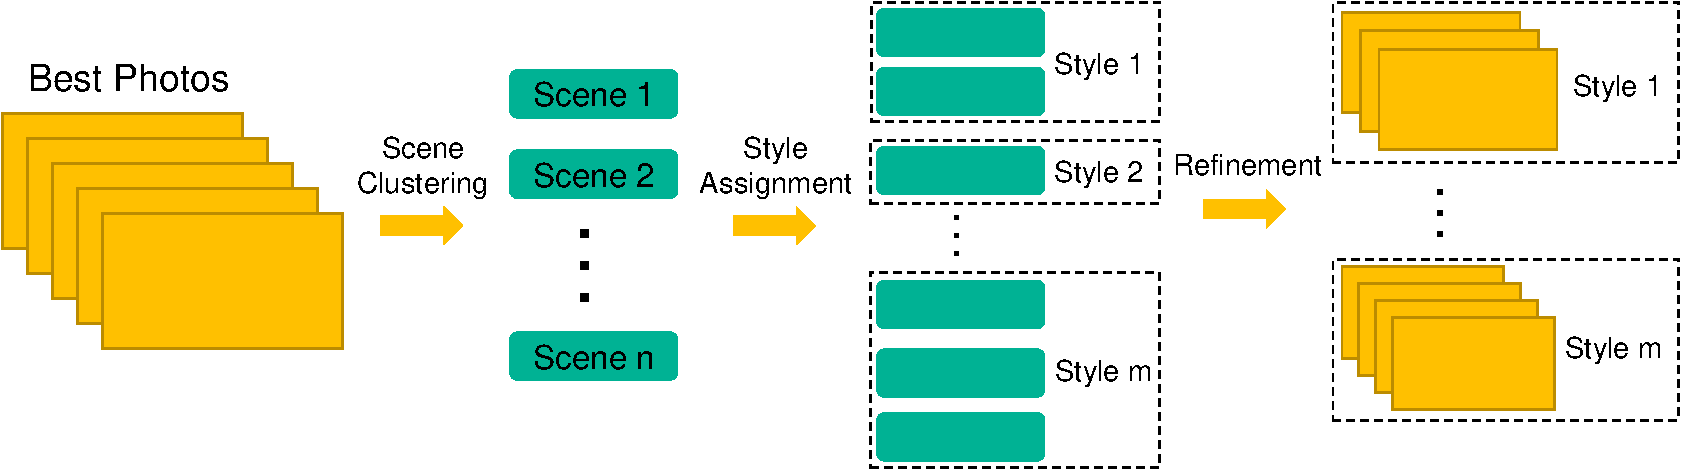
\includegraphics[clip=true, width=0.95\textwidth]{style-assignment.pdf}
    \caption{风格选取流程}
    \label{fig:style-assignment}
\end{figure}

\textbf{场景聚类}:根据我们与设计师讨论的结果,人们在特定场景中拍摄照片记录值得
纪念的时刻。换句话说,照片不仅被时间和位置信息显式地组织,同时也被场景隐式地组织。
我们的系统的主要目的是从场景中总结用户照片生成音乐视频。为了衔接照片和场景之间的联系,
每个照片用上节阐述的语义模型产生的概率向量表示$\p_i = (P(t_1|x_i), P(t_2|x_i), \ldots,
P(t_N | x_i))$。我们用Affinity Propagation(AP)~\cite{frey2007clustering}算法对照片聚类,
每个聚类中心被当做是一个场景。

\textbf{风格选取}:在我们的系统中,用不同的编辑风格表现不同的场景,使得故事化的表达
更加具有吸引力更加智能。为了决定每个场景需要使用什么编辑风格,我们用照片的语义特征训练
多类的SVM分类模型。我们邀请设计师设计了用户照片中最经常见的场景以及相关的语义词汇,如
``爱情''相关的词汇包括\emph{爱情,夫妻,甜蜜,婚礼,宝贝}。为了使得这些词汇表达的语义
是可计算的,我们用这些词从Flickr上获取至少$5,000$张照片,并用本文提出的语义理解模型将他们
提出他们的语义特征。我们训练了多类SVM分类器来区别不同的编辑风格。相应的,照片$x_k$
属于风格$\S_j$的概率表示为$P(\S_j|\p_k)$。

如果场景$scene_i$包含$M$张照片,$scene_i = \{\p_1^i, \p_2^i, \ldots,
\p_M^i\}$,该场景属于风格$\S_j$的概率为:
\begin{equation}
    P(scene_i, \mathcal{S}_j)= \sum_{k=0}^{M-1} P(\mathcal{S}_j|\textbf{p}_k^i) / M.
\end{equation}
最终,系统选取概率最大的风格编辑场景$scene_i$。
系统可能会给不同的场景选择相同的编辑风格,我们将相同风格场景的照片放到一起生成一个音乐视频。

\subsection{生成视频片段}
本文采用了Hua等人提出的照片生成视频片段的方法~\cite{hua2006photo2video},
主要包括三个步骤:
\begin{itemize}
    \item 关键帧选取。为了模拟相机运动,我们需要照片中选取全景,中景,近景作为关键帧。
    \item 生成关键帧序列。我们需要决定关键帧的播放顺序。基于电影制作的规则,我们采用了
        Hua等人提出的14种播放策略产生关键帧序列~\cite{hua2006photo2video}。
    \item 生成相机运动。最终的视频片段是通过在关键帧之间采用特定的相机运动实现的。
        对于一系列的照片,我们按照Hua等人提出的方法构建了一个合适度矩阵,通过
        最大化整体相机运动合适度和相机运动分布均衡性为每个照片选取合适的相机运动。
\end{itemize}

\subsection{音乐分析}
音乐视频需要将音乐的节奏和视频镜头的切换进行匹配。Monet系统首先对音频抽样到8kHz,
并通过Hua等人提出的方法检测音乐的节奏~\cite{hua2006photo2video}。
根据音乐的节奏和强度,系统检测最终音乐视频的切换点,从而决定生成的视频片段时长。
切换点是指音乐视频从一个视频片段切换到另一个的时间点。
切换点的检测算法将在~\ref{sec:mashup-cutpoint}中阐述,该方法提供了更好的音视频关联性,
使得视频片段的切换频率和音乐节奏更加协调。此外,该方法也尽量选择在歌唱的间歇切换,
与现有的方法在节奏点切换有明显的区别。

\subsection{故事合成}
为了生成专业的音乐视频,仅仅将视频片段和音乐混流是不够的。我们需要添加如特效,形状,
颜色过滤器,转场等视觉效果使得音乐视频更加平滑更加具有吸引力~\cite{mei2007videosense}。
为了达到这个效果,我们为每一个编辑风格设计了视觉特效模板,总结可计算的电影制作语法将
视觉效果添加到视频片段中。最终的音乐视频根据视频片段,音乐,和这些视觉特效生成。

\subsubsection{风格模板设计}
对于每个风格,我们设计了模板特效,形状,颜色过滤器和转场效果,每个视觉特效都依赖于具体
的照片内容。图~\ref{fig:monet-shape_et_example}显示了一些视觉效果的样例。
\begin{figure}[ht]
    \centering
    \subfigure[条纹效果] {
    
\includegraphics[width=0.23\linewidth]{multi-stripe.png}
    }
    \subfigure[叶子形状] {
    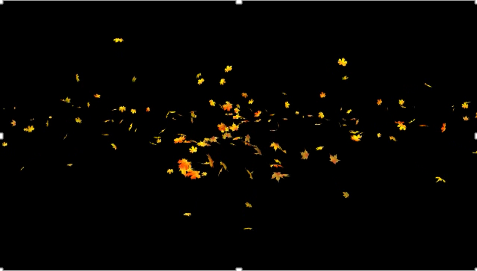
\includegraphics[width=0.23\linewidth]{shape.png}
    }
    \subfigure[阳光颜色过滤器] {
    
\includegraphics[width=0.23\linewidth]{color-filter.png}
    }
    \subfigure[圆形转场] {
    
\includegraphics[width=0.23\linewidth]{transition.png}
    }
    \caption{特效,形状,颜色过滤器,转场样例。
        (a)条纹效果将照片分割成条纹依次展现,是自然主题的一种表现手法。
        (b)叶子形状中,黄色的树叶缓慢地漂浮在视频中,唤醒用户对于原始和旧时光的记忆。
        (c)将照片和阳光颜色过滤器融合能够帮助用户体验自然主题下的阳光照耀的效果。
        (d)圆形转场逐步从中间到四周展现内容,能够有效地吸引观看者的注意力到照片中的主要物体或人物。
    }
    \label{fig:monet-shape_et_example}
\end{figure}

不同的视觉效果有不同的表达效果,适用于不同的语义内容。比如,
自然风格的条纹效果(图~\ref{fig:monet-shape_et_example}(a))
适用于户外拍摄的植物或天空,但不适用于包含人的照片,因为没有用户愿意人物照片
被分割成条纹。类似的,``原始''风格中的叶子形状(图~\ref{fig:monet-shape_et_example}(b))
适用于包含草地或者树叶的照片。
``聚会''风格的圆形转场(图~\ref{fig:monet-shape_et_example}(d))特别适合照片中间仅有
一个焦点人物或物体的照片,尤其是仅包含大比例人脸的照片。甚至有效视频效果尤其是转场效果
仅适用于特定的相机运动的视频片段。总之,不同的视觉效果对于不同的语义内容和相机运动有不同的
合适度,我们为每个风格的特效、形状、颜色过滤器和转场定义了合适度语法。特效的语法规则定义
如下xml格式(形状和转场的语法类似):
\begin{itemize}
    \item \textbf{根节点$<$Grammar$>$}:根节点包含风格信息,以及特效、形状
        和转场语法的子节点。
    \item
        \textbf{特效节点$<$Effect$>$}:特效节点描述特效相对于不同语义特征和运动的合适度。
        每个特效节点包含包含一个或者多个``condition''子节点和一个可选的``percent''子节点。
        ``condition''节点包含``feature''和``score''两个子节点。如果``feature''节点以``+''
        开头,则该特效适用于该特征,如果以``-''开头,则特效不适用。``score''子节点表示特效
        适用于该特征的程度。特效节点的``percent''子节点表明该特效在所有选择特效中
        适宜出现的比例。
\end{itemize}
如果视频片段包含不适合的特征,特效的合适度则为$0$,否则特效的合适度为所有特征合适度之和。
根据视频效果语法,我们可以计算每个视频效果和每个视频片段的合适度以及部分效果期望出现的比例。


颜色过滤器的语法稍有不同。即使对于相同的视频片段,
光照和颜色分布的变化也会导致不同的表达效果。
因此,我们设计为不同的风格设计了不同的颜色过滤器,语法格式为:
\begin{itemize}
    \item \textbf{视频颜色过滤器节点$<$ColorFilter$>$}:该节点描述以视频形式出现的
        颜色过滤器的信息。``path''子节点包含视频的路径,``opacity''子节点控制过滤器视频和
        视频片段叠加时的不透明度,``overlay''子节点包含叠加的方式,``minPercent''和``maxPercent''
        控制该视频过滤器出现的最少和最大比例。
    \item
        \textbf{图片颜色过滤器节点$<$ImageFilter$>$}:该节点描述图片颜色过滤器的信息。节点内容
        与视频颜色过滤器基本相同,除了``path''子节点被替换为``name''子节点,表明预先定义的
        图片颜色过滤器。此外,图片过滤器节点包含\textbf{特效节点$<$Effect$>$}节点中的``condition''节点。
\end{itemize}
为了计算视频颜色过滤器和视频片段之间的合适度,我们首先提取颜色过滤器视频和视频片段的显著图(saliency
map)~\cite{ma2003saliency},合适度通过显著图之间的负相关系数得到。换句话说,视频颜色过滤器
不应该将用户的注意力从照片的主题内容分散到颜色过滤器上。

\subsubsection{优化视觉效果分配}
视频效果的选取可以定义为一个优化问题进行求解。
假设一共有$N_c$个视频片段,每个视频片段表示为$c_i$,一共有$N_e$个视频效果,每个表示为
$VE_j$。选取视觉效果通过确定一个选择矩阵$X=(\x_1, \x_2, \ldots,
\x_{N_C})$,$\x_j$是一个$N_e$维仅包含一个非零元素的二值向量。由于不同的视觉效果
有不同的期望出现比例(percent),我们需要首先确定它们的期望选择次数$n_j^*$。
如果$VE_j$的期望比例为$p_j$,显然$n_j^* = p_jN_c$。如果$p_j$没有指定,我们根据
它们与视频片段之间的合适度确定出现比例。假设视频片段$c_i$和视觉效果$VE_j$之间的合适度
为$S_{ij}$,$VE_j$的整体合适度为:
\begin{equation}
    S_j = \sum_{i=0}^{N_c-1}S_{ij}(1 - I_j),
\end{equation}
$I_j$是一个指示向量,当$p_j$被指定时$I_j$为1,否则为0。$VE_j$预期出现的比例为:
\begin{equation}
    p_j = \frac{S_j}{\sum_{k=0}^{N_e-1}S_{k}(1 - I_{k})}p^*,
\end{equation}
$p^* = 1 -\sum_{k=0}^{N_e-1}p_{k}I_{k}$是没有被指定比例的视觉效果能够出现在视频片段
中的剩余比例。

视频特效的选取可以归结为一个最大化整体合适度和出现比例的优化问题:
\begin{equation}
    X^* = \argmax_{X}
    \sum_{j=0}^{N_e-1}d_j\frac{\sum_{i=0}^{N_c-1}X_{ij}S_{ij}}{n_j},
\end{equation}
$d_j = exp(-\frac{(n_j-n_j^*)^2}{2})$是出现比例的分数,
用以衡量视觉效果的出现比例和预期出现比例之间的差异。

然而,仅仅只最大化合适度和出现比例可能会导致相同的相同的视觉效果被分配到
连续的视频片段。为了保持视频片段原始的顺序,保证最终视频的故事性,同时防止这种连续
效果的单一性,我们对视频效果的分布均匀性进行约束。

假设$VE_j$在$N_c$个视频片段中出现$n_j$次,我们希望$VE_j$均匀地出现在视频中。因此,
选择$VE_j$的相邻视频片段之间的预期间隔为$\frac{N_c -
n_j}{n_j}$。假设选择$VE_j$的第$k$个和第$k+1$个视频片段之间的间隔为$\delta_k$,则$VE_j$
的均匀性分数$u_{jk}$定义为:
\begin{equation}
    u_{jk} = exp(-\frac{(\delta_{k}-\frac{N_c-n_j}{n_j})^2}{2}).
\end{equation}
相应地,整体的均匀性分数为:
\begin{equation}
    U = \sum_{j=0}^{N_e-1}\frac{\sum_{k=0}^{n_j-1}u_{jk}}{n_j^*-1}.
\end{equation}

考虑到合适度,出现比例和均匀性,视频效果选取问题归结为优化如下目标方程:
\begin{eqnarray}
    X^* = \argmax_{X_{ij}}
    \sum_{j=0}^{N_e-1}(d_j\frac{\sum_{i=0}^{N_c-1}X_{ij}S_{ij}}{n_j}
    + \lambda \frac{\sum_{k=0}^{n_j-1}u_{jk}}{n_j^*-1}).
\end{eqnarray}
我们使用回溯法求解上述优化方程的最优解。

经过对用户照片集的事件检测和关键照片选取,生成视频片段,匹配音乐,以及选取视频效果以后,
Monet系统生成最终的音乐视频,对用户的照片集进行总结,并按照用户主题对用户照片集进行故事化的表达。

\section{实验结果}
据我们所知,目前还没有其他完整的系统能够自动对用户照片集进行总结并创建故事化的表达。
为了评价Monet系统的有效性,我们从照片集总结和故事合成两个角度评价Monet系统。

在实验中,所有的照片都是从用户上传的照片集中选取。为了评价照片集总结算法的效果,
我们让上传者对他们的照片进行标注,找出照片集中的事件和关键照片,并将用户照片上传到
其他事件检测和关键照片选取系统获取它们的总结结果。对于故事合成,我们邀请用户从他们的
照片集中针对每个主题风格推荐照片。然后我们随机选取一个风格并将对应的照片和音乐提交到
Monet系统和其他系统中,通过用户调查(user study)评测不同系统生成的视频。

\subsection{事件检测和关键照片选取评测}
我们邀请了6名用户分享他们在过去两年拍摄的照片,所有的照片都包含准确地拍摄时间戳,
但只有一部分包含GPS信息。用户被要求将他们的照片按照事件进行分组。对与每个事件,
他们需要为每个事件选取他们最能代表这个事件的1到6张照片作为关键照片。
这些用户标注结果被当作评测事件检测和关键照片选取的真实数据。照片集的详细情况
如表~\ref{tab:monet-photos-info}所示。
\begin{table}[htbp]
    \centering
    \caption{用户照片集详细信息} \label{tab:monet-photos-info}
    \begin{tabular}{|c|c|c|c|c|c|c|}
        \hline
        Dataset & User 1 & User 2 & User 3 &  User 4 &User 5 & User 6\\ \hline
        \#Photos & 1080 & 481 & 496 &  564 & 702 & 866 \\ \hline
        \#Events & 95 & 32 & 40 &  107 & 28 & 58 \\ \hline
        \#Best Photos & 206 & 145 & 108 &  375 & 66 & 285 \\ \hline
    \end{tabular}
\end{table}

我们采用了准确率(Precision),召回率(Recall),
和F-score来评测事件检测的效果~\cite{cooper2005temporal}。准确率表示正确检测到的
事件边界比例:
\begin{equation}
    {\text{Precision}}_{seg}=\frac{\text{\#正确检测到的事件边界}}{\text{\#检测到的事件边界}}.
\end{equation}

召回率表示正确检测到的事件边界相对真实事件边界的比例:
\begin{equation}
    {\text{Recall}}_{seg}=\frac{\text{\#正确检测到的事件边界}}{\text{\#真实事件边界}}.
\end{equation}

F-score评价综合的性能:
\begin{equation}
    \text{F-score}=\frac{2\times \text{Precision} \times \text{Recall}}{\text{Precision} + \text{Recall}}.
\end{equation}

关键照片选取通过准确率(Accuracy)评价:
\begin{equation}
    \text{Accuracy}_{best} =\frac{\text{\#正确选取的关键照片}}{\text{\#真实关键照片}}.
\end{equation}

事件检测的结果如表~\ref{tab:monet-event-seg-res}所示。可以发现,
Monet在准确率和召回率上都比PhotoToc和TEC要好,因而也
有更高的F-score。高准确率和高召回率表明Monet不仅检测到容易发现的事件边界,也能找出较难
检测的事件边界。对于关键照片选取,Monet达到了$0.68$的准确率,高于目前现有的系统(如
Google+, OneDrive, Nokia StoryTeller等)换句话说,Monet能更准确地找出能够代表照片集的关键照片。
\begin{table}[htbp]
    \centering
    \caption{事件检测结果比较}
    \label{tab:monet-event-seg-res}
    \begin{tabular}{|c|c|c|c|}
        \hline
        Method          & Precision     & Recall    & F-score \\
        \hline
        PhotoTOC\cite{platt2003phototoc} & 0.50          & 0.71      & 0.59 \\
        \hline
        TEC\cite{cooper2005temporal}      & 0.39          & 0.54      & 0.45 \\
        \hline
        Monet                    & 0.85     &   0.72    & 0.78 \\
        \hline
    \end{tabular}
\end{table}

\subsection{故事合成评测}
故事合成的客观评测比较困难,我们通过主管用户调研的评价系统性能。Monet系统一共包含10
个主题风格,我们邀请用户从他们的照片集中为每一个主题风格推荐照片。
由于不是所有用户都有所有主题风格的照片,不同的主题风格的照片可能来自不同数目的用户。
为了比较系统性能,我们为每个风格随机选取一个用户的照片作为测试数据。然后,我们将
每个风格的照片以及相应的音乐上传到Monet, Animoto, Magisto,和Tilting Slide
Show系统中,因而最终能产生总共40个音乐视频。在Animoto系统中,照片被添加特效,在背景
音乐下一次展现。Animoto为照片之间添加了转场效果,但没有考虑相机运动。在Magisto系统中,
照片伴随特效,转场,相机运动和背景音乐一起播放。在Tilting Slide Show系统中,
照片以瓷贴的形式根据音乐的节奏展现。

我们邀请了20名用户(12名男性,8名女性,用户的年龄从22岁到28岁不等)
对一共10个主题40个视频进行打分。相同风格的视频在相同页面上
按照随机顺序展现给用户。
用户从以下方面对每个视频的满意度从1到7(分数越高越好)
进行打分:

\begin{itemize}
    \item 问题1:相机运动是否合理(对比专业视频)?
    \item 问题2:视频片段之间的转场是否平滑?
    \item 问题3:整个视频的视觉效果是否有吸引力?
    \item 问题4:视频片段之间的转场是否与音乐节奏匹配?
    \item 问题5:整个视频看上去是否像专业编辑的视频?
    \item 问题6:视频是否讲述了有趣的故事?
    \item 问题7:有多少可能你愿意分享该视频给你的朋友或社交网络?
    \item 问题8:你对该视频的整体满意度是多少?
\end{itemize}

所有问题的用户打分以及平均分如表~\ref{tab:monet-story-remixing-res}所示。前4个问题是关于
故事生成的具体方面。相比于Tilting Slide Show播放静态照片和Animoto简单的相机运动,
Monet和Magisto采用了更加专业的相机运动、更丰富的特效、形状和转场,
因而它们都获得了更高的评分。Monet在相机运动和转场上的评分略低于Magisto,其中一个原因
在于Monet根据当前照片的内容选取相机运动,转场根据之前和下一个视频片段选取,视频片段
切换点也基于马尔可夫假设来确定(详见章节~\ref{sec:mashup-cutpoint}),这些方面都是基于
局部信息的。我们猜测Magisto利用了一些全局信息或者优化方法来创建更加流畅和连续的视频,
使得最终的视频编辑更具有一致性。尽管如此,Monet仍然获得了和Magisto相差无几的评分。
在视觉效果的吸引力上,Monet获得了更高的分数,
验证了本文提出的风格模板在故事合成中的有效性。

后续的四个问题是关于不同系统的整体评分。尽管Magisto在相机运动和转场上效果略好,
Monet在视频编辑的专业性上仍然获得了最高打分,再次表明Monet系统视觉效果设计和选取的
优越性。由于Magisto实现了更加平滑的转场和相机运动,它在故事性上表现更优。
尽管如此,用户在分享视频的评价上仍然更加倾向Monet系统。Monet系统在整体满意度和
平均满意度上也获得了最高的评分。这些结果表明:
1)视觉效果对于生成专业的有吸引力的视频至关重要;
2)在其他方面,Monet与当前最好的Magisto系统表现相当。
3)整体来说,Monet在照片集故事化表达上获得了最好的满意度。

\begin{table}[htbp]
    \centering
    \caption{故事生成主观评测结果}
    \label{tab:monet-story-remixing-res}
    \begin{tabular}{|c|c|c|c|c|c|c|c|c|c|}
        \hline
        & Q1 & Q2 & Q3 & Q4 & Q5 & Q6 & Q7 & Q8 & Average  \\
        \hline
        Magisto & \textbf{5.83} &\textbf{5.67} & 5.33 & \textbf{5.78} & 5.67 & \textbf{5.22} & 5.05 & 5.54 & 5.51 \\
        Animoto & 4.5 & 5 & 4.33 & 5.11 & 4.28 & 3.8 & 4.17 & 4.56 & 4.47 \\
        Monet & 5.78 & 5.60& \textbf{5.83} & 5.67 & \textbf{6} & 4.94 & \textbf{5.28} & \textbf{5.72} & \textbf{5.60} \\
        TS Show & - & 3.62 & 3.22 & 3.05 & 2.9 & 2.5 & 2.56 & 2.83 & 2.59 \\ \hline
    \end{tabular}
\end{table}

\section{小结}
本文提出了一个端到端的从用户照片集中制作基于主题的故事化表达的系统Monet。
该系统能够自动总结用户照片集并按照电影编辑语法和预先定义的编辑风格,
以有趣味性和纪念意义的音乐视频的形式叙述照片集中的故事。该系统包含两个阶段:
用户照片总结和故事合成。在照片集总结阶段,我们首先提出了一个新的多模态生成模型将用户
照片划分成事件,其次,我们根据照片的美学质量,代表性,事件的重要性从每个事件中选取一部分
关键照片代表整个照片集。在故事合成阶段,为了叙述这些关键照片,我们使用分类模型将每个照片
分配到专业编辑人员预先定义的不同编辑风格中,并将属于同一个风格的照片重新组织起来。
对于每一个照片,我们选取了特定的相机运动将它转化为动态的视频片段。为了提高最终表达
的吸引力和平滑性,我们根据视频编辑语法和视觉内容将基于风格的视觉效果运用到
视频片段中。最终,我们将视频和音乐混流生成音乐视频作为照片集的故事化表达。

本章的主要贡献包括:
\begin{itemize}
    \item 提出了自动选取照片风格的模型,
        照片的风格选取被当前故事化表达系统忽视的关键部分;
    \item 根据电影编辑语法定义了一系列编辑模板,
        使得系统可以十分高效地运用视频特效;
    \item 首次引入了多个维度的信息(音频,照片,视频)生成精美的视频表达;
    \item 系统选取关键照片的部分可以节省大量用户浏览和选取照片的时间。
        该部分也使得该系统成为首个全自动照片集故事化表达系统。
\end{itemize}



\chapter{移动多摄像头视频自动剪辑}
\section{可计算视频编辑语法}
\section{移动多摄像头视频自动剪辑系统框架}
\section{音频剪辑}
\section{镜头切换点检测}
\section{视频镜头选取}
\section{实验结果}
\section{小结}


\chapter{总结与展望}
\section{本文总结}
\section{研究工作展望}

%%%%%%%%%%%%%%%%%%%%%%%%%%%%%%
%% 附件部分
%%%%%%%%%%%%%%%%%%%%%%%%%%%%%%

% 参考文献
% 使用 BibTeX
\bibliographystyle{ustcbib}%{GBT7714-2005NLang-UTF8}
\bibliography{bib/tex}
\nocite{*} % for every item



\appendix

\backmatter
\begin{acknowledgements}

在研究学习期间,我有幸得到了三位老师的教导,
他们是:我的导师,中国科大XXX研究员,中科院X昆明动物所马老师以及美国犹他大学的XXX老师。
三位深厚的学术功底,严谨的工作态度和敏锐的科学洞察力使我受益良多。
衷心感谢他们多年来给予我的悉心教导和热情帮助。

感谢XXX老师在实验方面的指导以及教授的帮助。
科大的XXX同学和XXX同学参与了部分试验工作,在此深表谢意。

\end{acknowledgements}


\begin{publications}

    \section*{已发表论文}

    \begin{enumerate}
        \item \textbf{Yue Wu}, Steven C.H. Hoi, Tao Mei, and Nenghai Yu. ``
            Large-scale Online Feature Selection for Ultra-high Dimensional Sparse
            Data'', ACM Transactions on Knowledge Discovery from Data
            (accepted).
        \item \textbf{Yue Wu}, Xu Shen, Tao Mei, Xinmei Tian, Nenghai Yu, and Yong
            Rui. ``Monet: A System for Reliving Your Memories by Theme-Based Photo
            Storytelling'', \emph{IEEE Transactions on Multimedia}, vol. 18, no.
            11, pp. 2206-2216, Nov. 2016 (the first two authors contributed equally).
        \item \textbf{Yue Wu}, Tao Mei, Ying-Qing Xu, Nenghai Yu, and Shipeng Li.
            ``MoVieUp: Automatic Mobile Video Mashup'', \emph{IEEE Transactions on
            Cirtuits and Systems for Video Technology}, vol. 25, pp. 1941-1954, Dec
            2015.
        \item Jianlong Fu, \textbf{Yue Wu}, Tao Mei, Jinqiao Wang, Hanqing Lu, and
            Yong Rui. ``Relaxing from vocabulary: Robust weakly-supervised deep
            learning for vocabulary-free image tagging'', In Proceedings of the
            IEEE International Conference on Computer Vision(ICCV), pp. 1985-1993,
            2015 (the first two authors are with equal contribution).
        \item \textbf{Yue Wu}, Shiyang Lu, Tao Mei, Jian Zhang, and Shipeng Li. ``Local visual
            words coding for low bit rate mobile visual search'', In Proceedings of
            the 20th ACM international conference on Multimedia (MM), pp.  989-992,  ACM, 2012.
        \item \textbf{Yue Wu}, Tao Mei, Nenghai Yu, and Shipeng Li.
            ``Accelerometer-based single-handed video browsing on mobile devices:
            design and user studies'', In Proceedings of the 4th International
            Conference on Internet Multimedia Computing and Service (ICIMCS '12).
            ACM, New York, NY, USA, 157-160.
        \item Dayong Wang, Pengcheng Wu, Peilin Zhao, \textbf{Yue Wu}, Chunyan Miao, and
            Steven CH Hoi. ``High-dimensional data stream classification via sparse
            online learning'', In Data Mining (ICDM), 2014 IEEE International
            Conference on(ICDM), pp. 1007-1012. IEEE, 2014.
    \end{enumerate}

    \section*{待发表论文}
    \begin{enumerate}
        \item \textbf{Yue Wu}, Steven C.H. Hoi, Chenghao Liu, Jing Lu, Doyen Sahoo,
            and Nenghai Yu. “SOL: A Library for Scalable Online Learning
            Algorithms”, Neurocomputing, 2016(Under review).
    \end{enumerate}

\end{publications}
\end{document}
